\documentclass[color]{tumphthesis}

\usepackage{duckuments}
\usepackage{epigraph}
\usepackage{lipsum}
\usepackage{wasysym}
\usepackage{cleveref}
\usepackage{subcaption}
\usepackage{graphicx} 
\usepackage{comment}
\usepackage{booktabs}  % nice looking tables
\usepackage{siunitx}


\thesistitle
{Analysis of unexpected Methane peaks in the urban environment of Hamburg}
{Der Titel meiner Magisterarbeit}
\thesisauthor{Juan Bettinelli}{Author}
\thesisdate{2023}{5}{14}
\supervisor{Prof. Dr Dopfer}
\examiner{Prof. Dr Chen}
\date{\today}


\begin{document}

\maketitle
\copyrightpage

\abstractpage
%\clearpage
%\chapter*{Abstract}
%\addcontentsline{toc}{chapter}{\protect Abstract}

Unexpected methane peaks in long-term continuous flow Isotopic Ratio Mass Spectrometer measurements (CF-IRMS) and in solar-tracking Fourier transform Infrared Spectrometer (FTIR) network measurements in Hamburg were investigated in detail.
A Keeling plot analysis of the prominent methane peaks from the CF-IRMS measurements with a concentration of over 2100 ppb and upto 4100 ppb showed an isotopic signature of $\delta$13C = -60.3$\pm $0.2$ \permil$ for Carbon-13 and $\delta$D = -298$\pm $2$ \permil$ for Deuterium. Indicating microbial methane production and pointing towards wetland and water bodies emitters.
Smaller peaks closer to the methane background concentration of 1921.74 ppb showed an isotope signature of $\delta$13C = -58.$\pm $0.1$ \permil$ for Carbon-13 and $\delta$D = -291.2$\pm $1$ \permil$, suggesting a stronger influence of methane production from thermogenic mechanisms, with potential sources being fossil fuels and nonindustrial combustion and other anthropogenic sources.
A purpose-built time-reversed Gaussian plume transport model using on-site measured wind data was used to model potential methane peak emission locations. The modelling indicated the most likely emission locations to be in the water bodies within and around the city; these include the port, channels, and wetlands.
An investigation into the water quality and water level data measured at the Elbe in the Hamburg port region showed a correlation between methane concentration in the atmosphere and the Elbe and its tidal cycle.
Correlations of meteorological data measured in the Hamburg city region and methane concentration in the atmosphere further indicate a significant influence of the water bodies in methane composition in the atmosphere in Hamburg.
This supports previous research by \cite{Matousu.2017}, who investigated the methane concentration in the Elbe estuary. They showed that the river produces a significant amount of methane in the upper estuary where Hamburg is located and observed that concentration in the water is enhanced with dropping  water levels due to the tide.
The spike in methane released into the atmosphere from methane and sediment-rich water bodies due to fast-dropping water levels has previously been investigated by \cite{Harrison.2017}. They postulated a release mechanism due to a rapid drop in water pressure and reduced water column height allowing for methane bubble formation in water and sediments, leading to diffusion into the atmosphere due to reduced methane oxidation potential. 
The Elbe estuary provides optimal conditions for similar rapid methane emissions to the atmosphere, making the Elbe the most likely source of the significantly high concentrated methane peaks observed in Hamburg. 
The high methane flux from the short-release events in the Elbe were observed as peaks with CF-IRMS in situ measurements at a distance of 5 km and a height of 83 m. The FTIR sensor network located in 4 different locations in the city was also able to observe methane peaks that likely originate from the Elbe. A good comparison between the two measurement approaches could unfortunately not be made due to limitations in the FTIR measurements and the short time of deployment. 










\tableofcontents

\mainmatter\setcounter{page}{1}
\chapter{Introduction}
\label{chap:intro}

Methane is one of the most dominant greenhouse gasses (GHG) in the Atmosphere and behind CO$_2$, the second most important anthropogenic greenhouse gas. It has a Global Warming Potential Value (GWP) of 81 for a 20-year horizon \cite{Forster.2021}, making it 81 times more potent than CO$_2$ for that time interval \cite{T.Stocker.2013}.\\
Methane is released into the Atmosphere in large quantities. Estimations suggest 363 Mt annual emissions \cite{IEA.4262023}. Various sources produce methane and release it into the Atmosphere, ranging from natural to anthropogenic. Natural methane emitters are considered ones where humane influence is not directly involved, such as microbial decomposition of organic materials in wetlands, volcanic activities or bound methane releases in permafrost deposits due to temperature rise \cite{Fernandez.2022}.  Anthropogenic sources are usually connected to using, transporting and treating fossil fuels, such as natural gas or oil. Fugitive releases from gas pipelines contribute to methane emissions significantly \cite{Schwietzke.2014}, \cite{McKain.2015}, along with other chemical industries and human infrastructure. This includes wastewater treatment, landfills, agriculture, and livestock. The methane present in the Atmosphere is always a mixture of all the different emitter types, particularly in densely populated regions.\\
Identifying and quantifying these emitters is of utmost importance to understand and predict the mechanisms that govern climate change and subsequently be able to create informed legislation to rein in runaway emissions that can permanently harm the atmosphere's equilibrium. \\
Hamburg is the second-largest city in Germany, with a population of around 2.5 million. The city has various urban uses, including typical residential areas with high and low-density neighbourhoods and extensive industrial, commercial, and port spaces. These industrial areas also include oil and gas refineries. Additionally, the city also provides numerous natural environments like parks and gardens. The extensive network of rivers, channels, lakes, ports and wetlands is a unique feature for a city 70 km inland.  The most prominent water body is the river Elbe. The Elbe connects the city to the North Sea, providing Europe's third-largest port, the Hamburg port, with a year-round navigable offshore shipping route. It has a diverse system of methane emissions sources that contribute to the methane composition in the air.\\
It is known that the Elbe is a significant methane emitter \cite{Matousu.2019}. The methane concentration in its water and release of methane into the atmosphere varies for the entire river. Its uneven distribution originates from many factors that will be discussed in further detail.\\
The river originates in the "giant mountains" in the Czech Republic. The first section is a natural fast-flowing river experiencing no impact by human influences. The river has no significant methane emissions in this region as the natural methane oxidation mechanisms are balanced with its production and influx mechanisms. In the second section, the river is heavily industrially used in the Czech Republic. The river is severely impounded in this section. The water has a high methane concentration due to pollution and few natural regeneration areas that form the feeding ground for good microbial methane oxidation. \\
The Third section describes the Elbe as a lowland river flowing through Germany. Groynes only stabilize its banks, and the river is significantly naturalized with free-flowing characteristics. In this section, the microbial methane production is kept in check with its countering oxidation processes, resulting in a low methane concentration in the water and consequent low atmospheric diffusion rates.\\
Some heavily impounded human-made structures are present throughout the river, including harbours, locks, and weirs. These sections form methane hotspots, as methane production is rampant due to the disturbed flow of the river and heavy pollution. At the same time, the oxidating mechanisms are repressed. The reason for the inability of oxidation is not fully understood yet and is most likely a multifactorial cause \cite{Matousu.2019}, \cite{Bednarik.2019}.\\
The river Elbe estuary starting at the city of Hamburg, down to the North Sea into the Waddensea, experiences different environmental factors, and different mechanisms drive its methane production and reduction mechanism. The upper estuary, including Hamburg's port, is defined by the heavily impounded region around Hamburg and experiences significant variations in water level due to the Tide. While no significant methane transfer from the saltwater of the Waddensea to the very nutrient-rich freshwater occurs in the upper estuary due to insufficient mixing \cite{Matousu.2019}. The water in this region has a short turnover time, with a very high methane concentration, similar to other harbours and human-altered segments upstream. The water has high pollution and biomass concentration from industry, agriculture, and other human and natural influences upstream and in the region. This high concentration of pollutants and biomass significantly enhances the methane production mechanisms while hindering the Oxidation mechanisms. High heterotrophic activity is related to remineralization processes of high loads of labile organic matter, and it has been shown by \cite{Matousu.2019} that the methane concentration in the Upper estuary correlates with BOD-7 (a measure of bioavailability of degraded organic matter). \\
This is further amplified by its short turnover time, where the oxidation processes have little time to take effect and efficiently remove methane from the system.\\
The river is significantly widened in the lower estuary, with an extensive network of connected marshlands. The marshland has methanogenic bacteria that are well-adjusted to the colder climate of northern Germany. Those can be found in oxic as well as in anoxic soil layers. Resulting in a methane production peak at 10 °C and 20 °C. \cite{Wagner.1997} The low-temperature peak production occurs due to reduced methane oxidation at low temperatures. Marshlands systems usually peak in a 30 °C region in warmer climates. \\
The water turnover time is significantly longer, providing good conditions for methane oxidation and greater methane diffusion into the atmosphere, resulting in a ten times lower methane concentration than in the upper estuary \cite{Matousu.2019}. A significant amount of the methane in the lower estuary originates from the Waddensea, as the tides flush highly methane-enriched water into the estuary. The well-functioning oxidation processes in this region would otherwise dominate the methane balance.\\
Low water levels in the river and high temperatures enhance microbial activity and thus decrease oxygen levels in the water. This can, for example, be observed in the seasonal cycle. While no apparent relation to suspended particular matter can be seen, the sediment has a significant role in the methane cycle. For example, Methanotroph reduces CH$_4$ Emissions from the sediments.  As one can observe from tidal activities, resetting the sediments significantly increases methane production due to the reintroduction of biomass and ions to the sediments \cite{Bednarik.2019}. The types of methane-producing microbe can vary significantly due to the type of sediments and vary significantly throughout the river, allowing them to form hotspots.\\
The water level also contributes to the methane balance. Low water levels reduce the ability of the water to oxidize the methane due to its lower water column height over the sediments. In the Elbe estuary, the methane concentration in the water is correlated to falling water levels due to the Tide. It is reaching its peak at the lowest water level. \cite{Harrison.2017} have shown that the fast reduction of the water level increases the methane concentration and, consequently, its emission to the atmosphere. \\
A possible explanation is that the thick sediment layers can accumulate a large amount of methane. The drop in pressure due to the reduction in water column height causes the methane to form bubbles, which are released from the sediments and travel up to the surface and escape to the atmosphere. The reduced water column height can no longer oxidize most of this methane, consequently defusing the methane into the atmosphere. The exact condition required for such a surge in methane emission is not yet detailed. It is most likely a function of sediment characteristics, water depth, lowering rate, etc.\\
For the Elbe estuary, it is estimated that 5–41 \% of the total methane loss in the water is attributed to active methane oxidation. The remaining part is released into the atmosphere due to diffusion \cite{Matousu.2019}.\\
The United Nations environment programme (UNEP) measurement campaign aimed to quantify the emissions in the city region of Hamburg, Germany. While providing the opportunity to compare and validate different data acquisition approaches with the best bottom-up inventories currently available.\\
The campaign was conducted between 01.08.2021 and 1.04.2022, with some short 1-3 day maintenance breaks. High time-resolution mass spectrometer measurements were conducted during the campaign, focusing on Deuterium ($^2$H) and Carbon 13 ($^13$C) isotopes. The measurement was stationary on the roof of the Geomatikum building owned by Hamburg University near the city centre, with a measurement inlet height of 83 m \cref{TimelineNoPeaks}.
\begin{figure}[htbp]
 \centering
 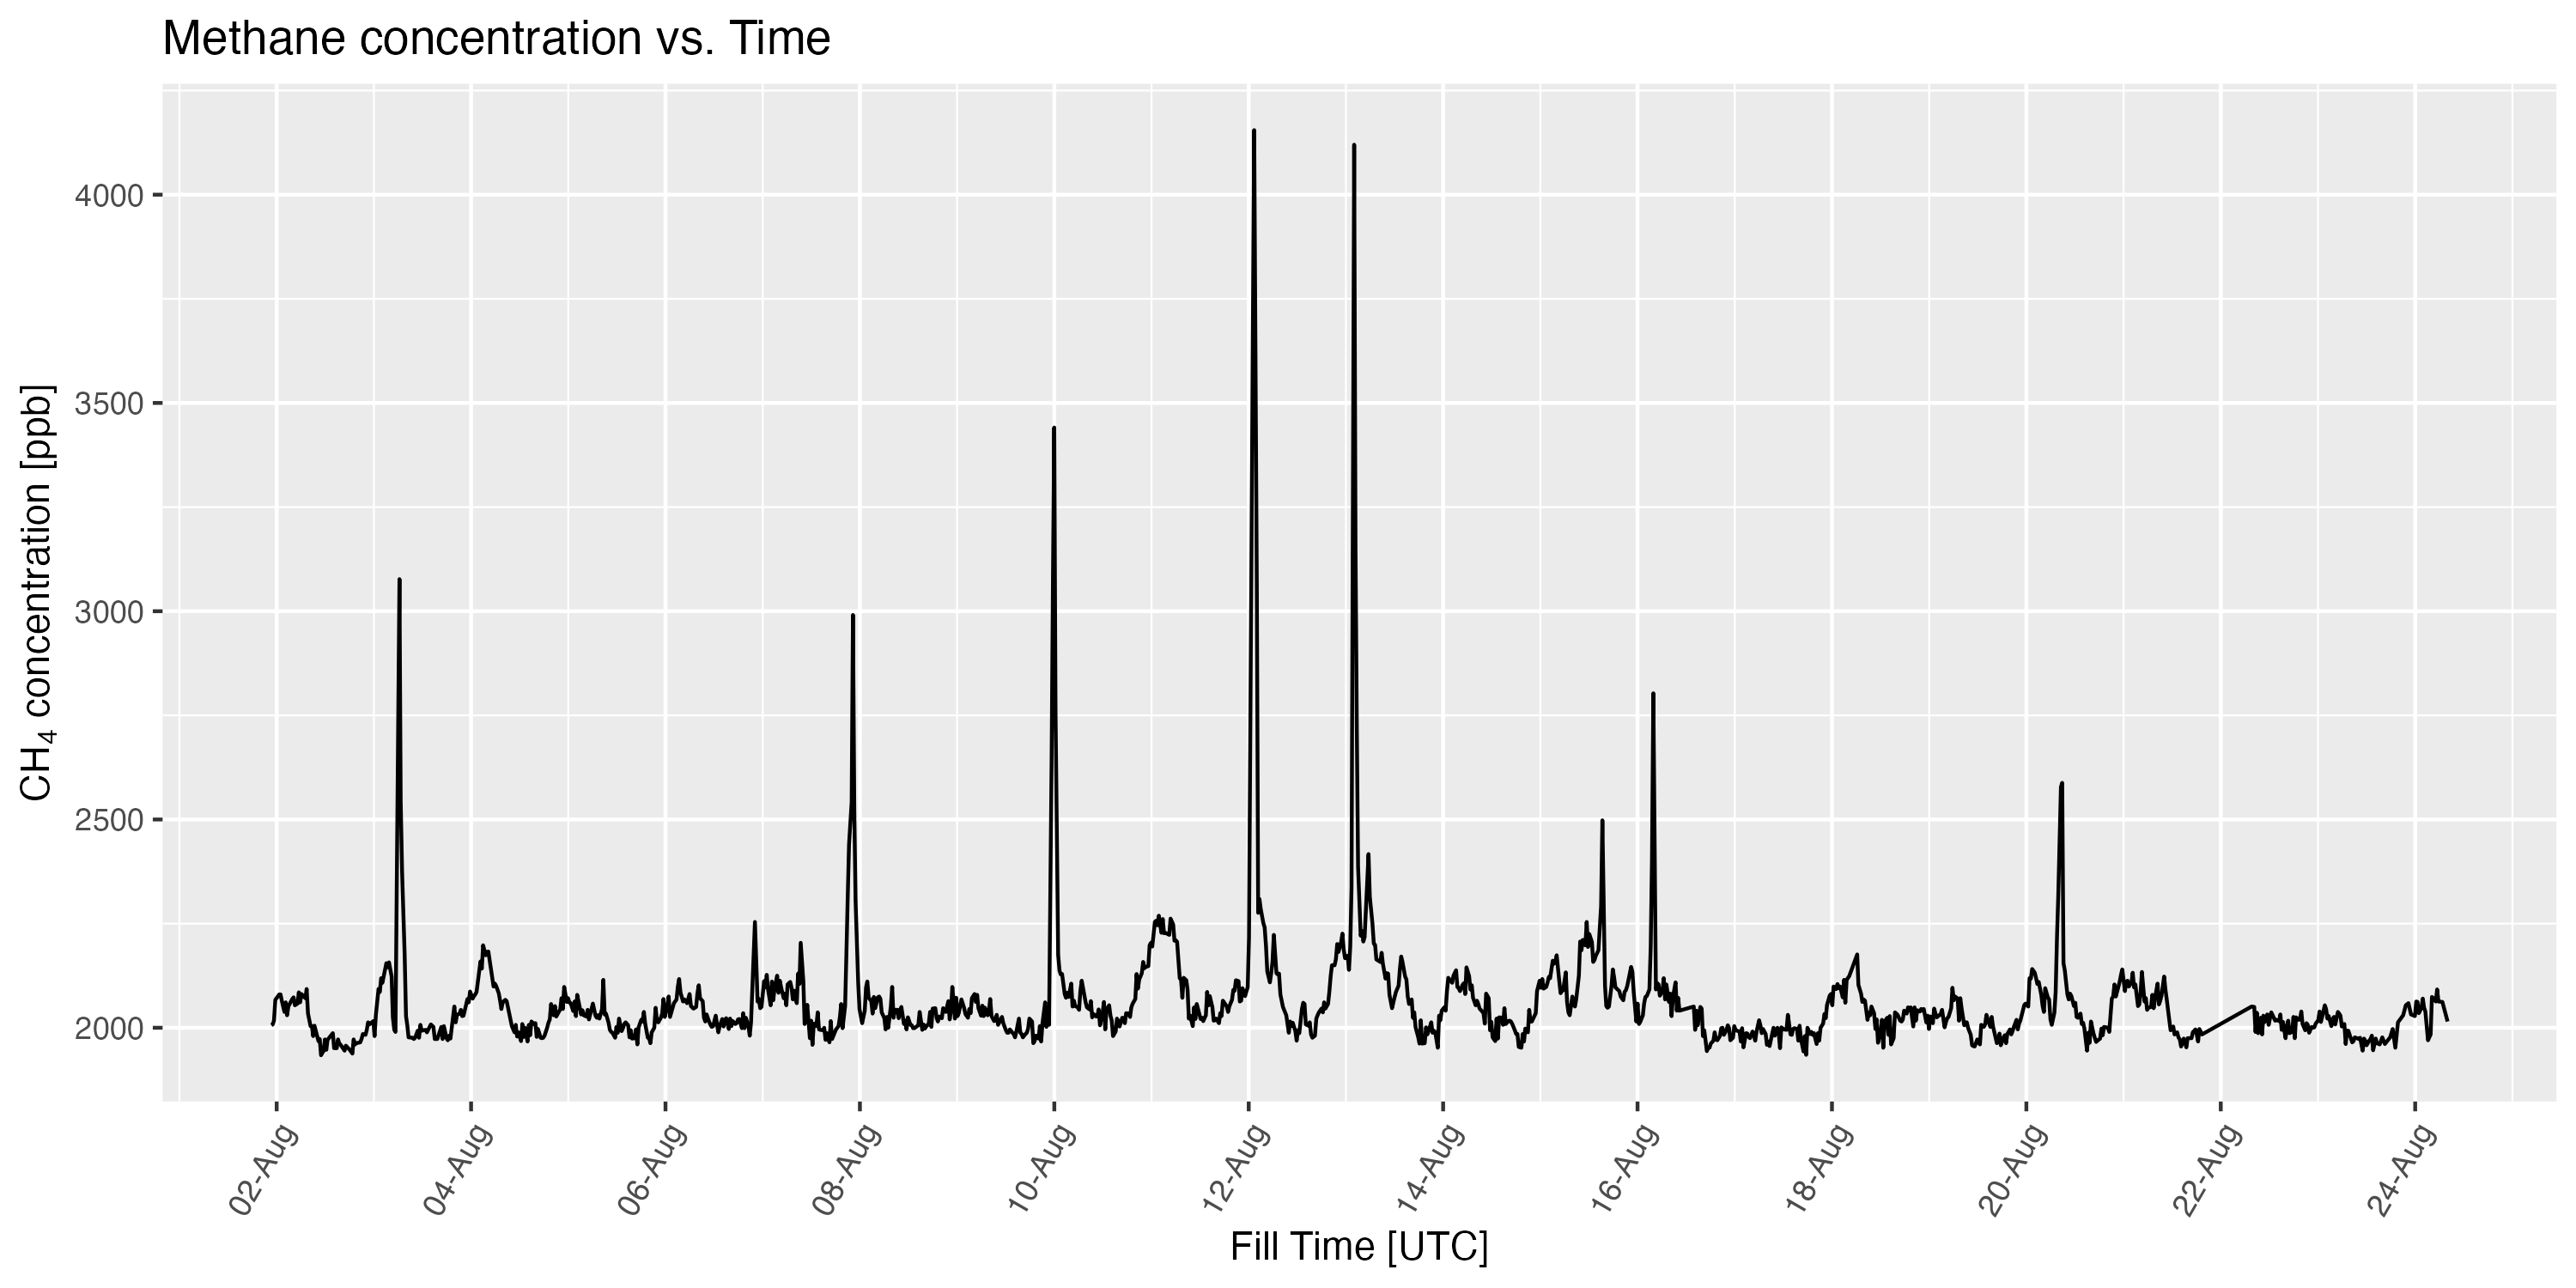
\includegraphics[width=1\textwidth]{figures/Appendix/CH4_Timelines/4_CH4_Timeline0_No_Peaks.png}
 \caption[CH$_4$ Timeline]{Section of CF-IRMS in situ measurement showing the timeline of methane concentrations measured in Hamburg Geomatikum (83m above ground) from 02.08.2021 to 24.08.2021.}
 \label{TimelineNoPeaks}
\end{figure}
A series of additional measurement approaches were conducted for the shorter period of 27.07.2021 to 9.09.2021. These include a solar-tracking Fourier Transform Infrared Spectrometer (FTIR) Network with four EM27/Sun spectrometers in and around Hamburg. This network enabled a differential total column measurement using the Bayesian inverse modelling approach. A Leosphere Windcube 200S Doppler wind LIDAR was also deployed to improve the transport modelling of the Bayesian inversion by correcting the atmosphere Boundary layer height and the wind direction of the wind model. \\
Mobile methane measurements by car and boat were also conducted to validate and improve the inventory for the uses as prior in the Bayesian inverse modelling.  A Picarro model G2301 measured mole fractions of CH$_4$, CO$_2$ and H$_2$ at a frequency of 0.3 Hz and a Picarro model G4302 measured mole fractions of C$_2$ H$_6$, H$_2$ O and CH$_4$ at frequencies of 1 Hz. The mobile measurements mainly focused on the industrial and port region in the south of Hamburg, filling the gaps left by a previous measurement campaign with the same approach, primarily focusing on the residential areas to the north.\\
The Isotope measurements and, to some extent, the FTIR measurement yielded some surprising results for their methane concentration that could initially not be explained. In particular, some seemingly randomly occurring high methane concentration peaks were observed. These peaks had a dry air mole fraction of up to 4500 ppb, while the average background was around 2000 ppb. The duration of the peaks was also concise, lasting for only around 0.5-3 h. The current global average mole fraction of methane is at 1921.74 ppb (January 2023) \cite{Lan.2022}.\\
By investigating the chemical composition of the methane by the Keeling method from Air sampled during the peaks, it was concluded that emission sources were due to natural microbial methane production mechanisms. Pointing towards wetlands and water bodies.\\
A purpose build particle transport model pointed towards emissions origination in the region of the city where the port, fleets, channels, and wetlands are located. \\
The occurrence of the peaks has been successfully correlated to the water level of the Elbe, as these regions experience strong water level fluctuations due to tidal effects. \cite{Harrison.2017} shows that a fast-dropping water level can trigger significant methane emissions into the atmosphere at freshwater reservoirs. Additionally, \cite{Matousu.2019} shows that the methane concentrations in the water of the river Elbe increase at dropping water levels.\\
Further correlations of meteorological and water quality data with the methane concentration in the Air provide an overall concrete conclusion of the origin of methane peaks. Linking it to the water bodies and wetlands in and around the city due to a complex interplay of man-made riverbank impoundments, pollution in the water, flow characteristics of the river sediment depositions and tidal influences.\\
The river Elbe is currently underrepresented in methane inventories. This is also suggested by \cite{Forstmaier.2023}, in which the methane modelling is significantly improved by including the river in the inventory. While the fluctuations of methane release by rivers and wetlands due to tidal effects are not well investigated and understood yet. This thesis shows their observable effects and the conclusion linking methane concentrations in the air to the river Elbe while providing ideas for further research.

\chapter{Method}
\label{chap:2}

\section{The UNEP Campaign}
The United Nations environment programme (UNEP) measurement campaign aimed to quantify the total type-based (natural and anthropogenic) methane emissions of Hamburg \cite{Forstmaier.2023}. Three measurement types were deployed during this campaign. A total column-based Fourier-Transform Infrared Spectrometer network, deployed from 27.07.2021 to 9.09.2021. A continuous flow isotope ratio mass spectrometer (IRMS) measurement at the Geomatikum from 01.08.2021 to 1.04.2022, a mobile dual Cavity Ring-Down Spectrometer measurements by car and boat from 09.08.2021 to 21.08.2021.\\
The FTIR sensor network is part of the Munich Urban Carbon Column Network (MUCCnet) and was relocated for the measurement campaign to Hamburg. The coordination and deployment were provided by the Technische Universität München (TUM) from Andreas Forstmaier (TUM) and Jia Chen (TUM). The sensors used in the MUCCnet are solar-tracking absorption spectrometers (Bruker, EM27/SUN) that enable column-averaged dry air mole fractions measurements of CO$_2$, CH$_4$, and O$_2$ \cite{Chen.2016}. A Bayesian inverse modelling approach was used to estimate the location and type-based methane emissions. The TNO GHGco inventory (Super et al. [2020]) was used as Prior information for the Bayesian approach. The inventory was further improved for the modelling by the results of the mobile survey. The ERA5 model \cite{Hersbach.2023} was used to model the transport by the atmosphere. The Wind lidar measurements were used to correct this model further. The wind lidar deployed was the Leosphere Windcube 200S Doppler wind LIDAR provided and operated by Norman Wildmann from the Deutsches Zentrum für Luft- und Raumfahrt (DLR) \cite{Wildmann.2020}, \cite{Vasiljevic.2016}.\\
The Isotope Ratio Mass Spectrometer system at the Geomatikum was provided by the Universiteit Utrecht and operated by Carina van der Veen. The Spectrometer used was a ThermoFinnigan MAT Deltaplus XL isotope ratio mass spectrometer, alternating $^2$H and $^{13}$C measurements with a frequency of 20 min. The measured Isotope ratios were analysed using a Keeling plot approach and compared for identification to a stable isotope ratio database of isotope measurements of known source types \cite{Menoud.2021}. \\
The mobile measurement survey deployed two Cavity Ring-Down Spectrometers, the Picarro model G2301 and a Picarro model G4302. Additionally, methane plumes were analysed by sample bags for their source attribution. The bags were examined with the isotope ratio spectrometer in the Geomatikum. Hossein Maazallahi from the Universiteit Utrecht conducted the mobile measurement survey. The survey completed a previous campaign performed with the same instrumentation in 2020 \cite{Maazallahi.2020}, concentrating on the northern parts of Hamburg, primarily residential areas. The measurements conducted between 09.08.2021 and 21.08.2021 focused on the southern regions with mostly industrial and port areas, surveying 1567 km.

\section{Continuous-flow isotope ratio mass spectrometry (CF-IRMS)}
The isotopic ratio signatures of Deuterium ($\delta$D) and Carbon-13 ($\delta ^{13}$C) were measured by using a continuous flow Isotopic Ratio Mass Spectrometer (CF-IRMS).  Isotope measurements are well suited to provide additional information about the production mechanism of methane since different sources emit CH$_4$ with a characteristic and, in many cases, distinct isotopic composition.\\
The system used is described in great detail by \cite{Brass.2010}, nether the less the analysis method is briefly described here to give a general inside. The method used is designed for a multi-month operation with minimal user interaction. Apart from liquid nitrogen refilling, which is used for cooling, the process is fully automated and continuously measures autonomously. Besides a few short 1-3 day maintenance beaks in which the furnace had to be replaced, the setup measured uninterrupted for the extended time period from 01.08.2021 to 1.04.2022. The isotope ratio determination procedure follows seven steps based on extracting and purifying the methane before analysing it with the mass spectrometer. \cite{Brass.2010}.
\begin{enumerate}
  \item In the first step, the air is sampled with a fixed volume of 40 mL.
  \item The methane is then pre-concentrated. This separates the methane from the bulk air. The separation process is performed by cooling the air to -130 °C. At this temperature, CH$_4$ condensates while N$_2$ and O$_2$ stay gaseous and can be separated mechanically. The remaining air is then heated to -85 °C, where the CH$_4$ becomes a gas again, but N$_2$, O$_2$, CO$_2$, H$_2$O and other condensable gases stay solid/liquid and are again mechanically separated by valves.
  \item The CH4 is focused in a small volume by recooling the methane. This also ensures a better separation from the O$_2$, N$_2$, and CO$_2$, which can harm the conditioning of the furnaces or cause interferences in the mass spectrometer. By reheating the CH$_4$, the release peak can be shortened, which ensures a high enough concentration in later processes. 
  \item The CH$_4$ is gas chromatographically separated by a PoraPLOT Q column from the remaining gas components.
  \item CH$_4$ is converted to either CO$_2$ or H$_2$, the two processes are alternated with a 20 min frequency. The CH$_4$ is combusted into CO$_2$ for the ${^{13}C}/{^{12}C}$ ratio analysis. In this process, the CH$_4$ is broken into CO$_2$+ H$_2$O. For the ${^{2}H}/{^{1}H}$ ratio analysis, the CH4 is converted to C+ 2H$_2$ via pyrolysis. This process uses highly purified Helium (He) (purity 5.0) as a transport medium.
  \item The converted CH4 is injected into the mass spectrometer via an open split interface 
  \item The mass spectrometer measures the molecular ion current ratios. The peak areas are evaluated for a methane concentration analysis.
\end{enumerate}
\begin{figure}[htbp]
 \centering
 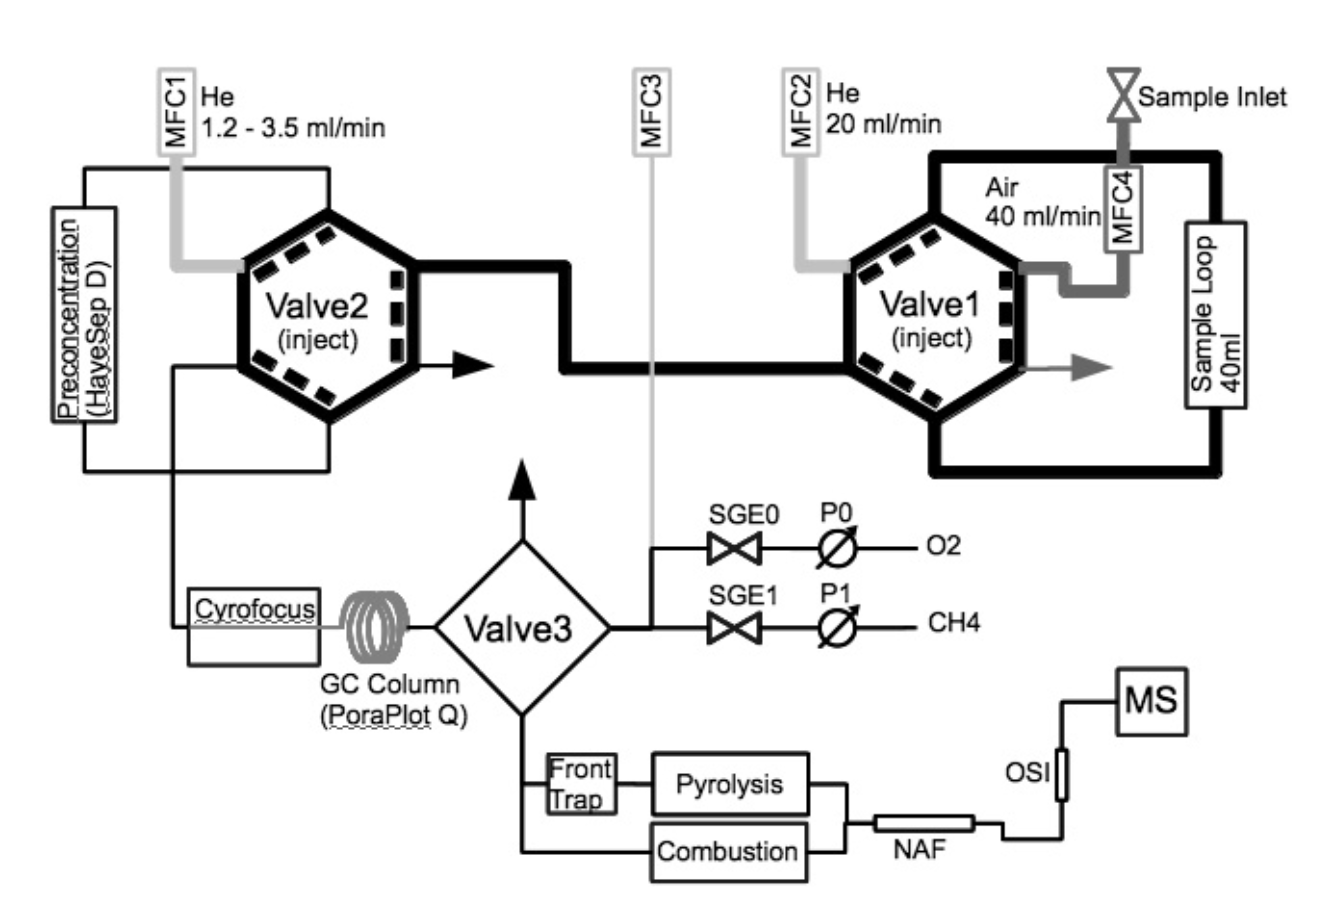
\includegraphics[width=1\textwidth]{figures/Methode/CF-IRMS_schematics.png}
 \caption[CF-IRMS schematics]{Schematics for the Continuous-flow isotope ratio mass spectrometry (CF-IRMS) deployed at the Geomatikum. Methane is isolated from other air components by subsequent preconcentration, cryo-focussing and gas chromatographic separation. The separated methane is then either combusted to CO$_2$ (for ${^{13}C}/{^{12}C}$ ratio analysis) or pyrolyzed to H$_2$ (for ${^{2}H}/{^{1}H}$ ratio analysis) and injected into the isotope ratio mass spectrometer for isotopic analysis. \cite{Brass.2010}}
 \label{CFIRMSSschematics}
\end{figure}
For calibration and stability monitoring, the isotopic ratio mass spectrometer measurement is packaged into six individual measurements (Reference-Sample-Sample-Sample-Sample-Reference). A complete measurement cycle takes About 20 minutes, and the $\delta ^{13}$C and $\delta$D measurements are alternated. The system pressure is also measured with a pressure sensor to determine the methane concentration of the sample air.

\subsection{Mass Spectroscopy}
The commonly used analytical technique of mass spectroscopy offers an excellent tool for measuring ion mass to charge ratio. This allows for accurate measurement of the isotope ratios in a sample, giving great insight into the production mechanisms of the molecules studied. By measuring and analysing the ratios of Hydrogen ($^{1}H$) to its heavier Deuterium ($^{2}H$) isotope and Carbon ($^{12}$C) to its heavier Carbon-13 ($^{13}$C) Isotopes in methane, its origin can be estimated. Further detail on this analysis process will be given later in the section on Keeling plot analysis.\\
A mass spectrometer can measure the charge ratio of an uncharged molecule by ionising the molecule by electron impact. The ionised molecule now has an electric potential and can experience the effects of magnetic and electrostatic fields.\\
The ions are accelerated using an electric potential, resulting in a similar Kinetic energy for all ions independent of their mass-to-charge ratio.\\
A magnetic field ($B$) is then applied to the accelerated ions resulting in a Lorenz force experienced by the ions. Consequently, the trajectory of the ions is bent towards a circle within the magnetic field. While equal charges ($q$) with an equal velocity ($v$) experience the same Lorenz force, they do not necessarily follow the same Circular trajectory and have the same radius ($r$). This is co-dependent on the mass ($m$) of the charge, i.e. the ionised molecule or atom. Hence for isotopes with larger masses, the radius of the trajectory differs from the radius of the lighter parent isotope. The heavier isotopes have a larger radius than their lighter contra part.
\begin{equation}
\frac{m}{q} = \frac{r \times B}{v^2}
\end{equation}
A continuous flow of ions on the magnetic field generates a mass spectrum on a detector (Ion collectors), a histogram of the isotope abundance/intensity versus its mass-to-charge ratio.\\
The mass spectrometer measures the Isotope ratio $\delta$X, which is noted in $\permil$. The isotope ratio describes the ratio of two isotopes ($R = {^{13}C}/{^{12}C} \ or \ R = {^{2}H}/{^{1}H}$) in a sample relative to the same ratio in a reference/standard material. 
\begin{equation}
\delta X = \frac{R_{sample} - R_{standard}}{R_{standard}}
\end{equation}
Due to the high cost and scarcity of well-defined and peer-reviewed reference samples, the measurements are performed against a working standard (WS). This Working standard is calibrated to a small amount of a well-defined reference with the mass spectrometer that will be used in the sample measurements.
The measured Isotope ratio of the sample can, later on, be converted to the international isotope scale (IS)by: 
\begin{equation}
\delta_{\frac{sample}{IS}} = \delta_{\frac{WS}{IS}} \delta_{\frac {sample}{WS}} + \delta_{\frac {WS}{IS}} + \delta_{\frac {sample} {WS}}
\end{equation}
The measurement results can then be published on the international isotope scale. The uncertainty in the reference sample and the instruments have to be accounted for when such an approach is implemented. For $^{13}$C
the international Isotope scale is the Viana Pee Dee Belemnite(VPDB), and for $^{2}H$, the IS is the Vienna Standard Mean Ocean Water (VSMOW).\\
By comparing the area of an isotope peak in the mass spectrum in the sample to a well-calibrated working standard reference of this spectrometer, the concentration can be calculated as follows:
\begin{equation}
c_{sample} = c_{WS} \frac{peak\  area_{sample}}{peak\  area_{WS}}
\end{equation}

\subsection{Keeling plot methode}
%needs rewriting!!!!!!
%%%%%%%references!!!!!!!!!!!!!!!
Charles D. Keeling showed in the fifties that the isotopic abundance of $ ^{13}C$ and $^{18}O$ can be correlated to the plant-based origin of CO$_2$ \cite{CharlesDKeeling.1958}, \cite{CharlesDKeeling.1960}. He devised a method for estimating the production mechanism of CO$_2$ by reference databases. This method was later adopted for methane. The abundance of heavy isotopes of 13C and 2H in a methane molecule enables the source type attribution \cite{Menoud.2021} \cite{Menoud.2022b}.\\
For methane, a strong depression in both $^{13}C$ and D ($\delta ^{13}C \sim {-60} \permil,  \delta D \sim {-300} \permil$), for example, can be observed in biological processes like boreal and tropical wetlands, rice cultivation, ruminants and waste decomposition. Natural gas and coal mining are thermogenic processes which have a strong enrichment in both heavy isotopes ($\delta ^{13}C\sim {-40}\permil,  \delta D\sim {-150}\permil$). Methane from biomass burning is unusually enriched in $^{13}C$ ($\delta ^{13}C\sim {-25}\permil,  \delta D\sim {-230}\permil$). Methane extracted from gas hydrates usually shows depleted 13C but enriched in D ($\delta ^{13}C\sim {-60}\permil,  \delta D\sim {-200}\permil$) \cite{Brass.2010}.\\
To analyse the isotope ratios measured by the CF-IRMS using the Keeling method, the currently most up-to-date database from \cite{Menoud.2022} is used as the comparison reference.\\
The mass spectrometer provides an isotope ratio $\delta$X in $\permil$ between the light and heavy stable isotopes. For methane, $\delta ^{13}C$ for $^{13}C$ and $^{12}C$ and $\delta$D for D and $^{1}H$ are used.\\
The Keeling plot approach is a mass balance and mass conservation approach. It considers methane concentration in the air (c$_a$), measured by the CF-IRMS, as a sum of the background concentration (c$_b$) and the concentration added by the source (c$_s$).
\begin{equation}\label{massconservation}
c_a = c_b + c_s
\end{equation}
By using the Isotope ratios $\delta$X for the heavy isotopes, the mass balance equation is constructed:
\begin{equation}\label{massbalance}
\delta_a c_a = \delta_b c_b + \delta_s c_s
\end{equation}
Combining \cref{massconservation} and \cref{massbalance} the yields:
\begin{equation}\label{keeling}
\delta_a  = \frac{c_b}{c_a} (\delta_b  - \delta_s) + \delta_s
\end{equation}
\cref{keeling} shows a linear correlation between the measured isotopic ratio $\delta_a$ and the inverse measured concentration $c_a$. The Y intersect represents the isotopic ratio $\delta_s$ of the source. This value can be compared to the reference values from a database. A Keeling plot is produced by scatter plotting a series of measurements with the Y axis as the measured isotopic ratio and the X axis as the inverse measured concentration. With an orthogonal distance regression line fit, the Y intersect, i.e. the isotope ratio of the source, can be obtained. For a comprehensive methane analysis, the source isotope ratio for carbon-13 $\delta ^{13}C$ and Deuterium $\delta$D has to be considered. \cite{Liu.2019} For better visualisation, both isotope rations can be plotted in a dual isotope plot, as seen in \cref{DualIsotiotopeTotal}.

\subsection{Keeling for methane peaks}
To investigate if there is a difference in source attribution between the background methane and the peaks, the Keeling analysis was performed by separating the peaks and the background with a peak finder algorithm. This allowed separating the peaks from the background and producing Keeling plots for the total measurement, background and both peak identification criteria separately. The results could be compared using reference isotope databases, and the emission mechanism could be estimated individually.

\subsection{Keeling analysis with wind}
Using the Keeling method for the background and peaks isotope measurement combined with Wind measurements, it was attempted to identify any anisotropic behaviour in the methane production.\\
The isotope measurements were binned according to the averaged wind direction during the measurement time. To achieve this, wind measurements at the Geomatikum provided by the Universität Hamburg were used for this. The wind measurement instruments were located very close to the isotope measurement inlet, allowing for high confidence in their relatability.\\
The isotope measurement bins were in 10° wind directions. For each bin, a Keeling analysis was performed separately. The results were then plotted in a dual isotope plot. In this plot, the Y intersect represents the $^2$H attribution, and the X represents the $^{13}$C attribution. The location of the binned points then indicates the methane production mechanism and emitter type when overlaying reference database data \cite{OwenA.Sherwood.2020} provided by the Global Monitoring Laboratory. A wide spread of the data points indicated different methane production mechanisms. While closely spaced points indicated homogenous emitter types in all directions.\\
By separating the methane peaks from the background and repeating the wind-sensible Keeling analysis, it can be investigated if the peaks from different directions originate from different emitter types.

\section{Differential column measurements}
A Fourier transform Infrared Spectrometer network was deployed inside and around the city borders to investigate the urban greenhouse gas (GHG) emissions from the city region of Hamburg. Parts of the usually in Munich located sensor network MUCCnet have been relocated to Hamburg and were deployed for a shorter period between 27.07.2021 to 9.09.2021. The network consists of four fully autonomous and automated Enclosures. These were located about 20 km from the city centre to the East, South and West, with one enclosure close to the city centre at the Geomatikum close to the mass spectrometer. The location can be seen in \cref{UNEPmap}.
\begin{figure}[htbp]
 \centering
 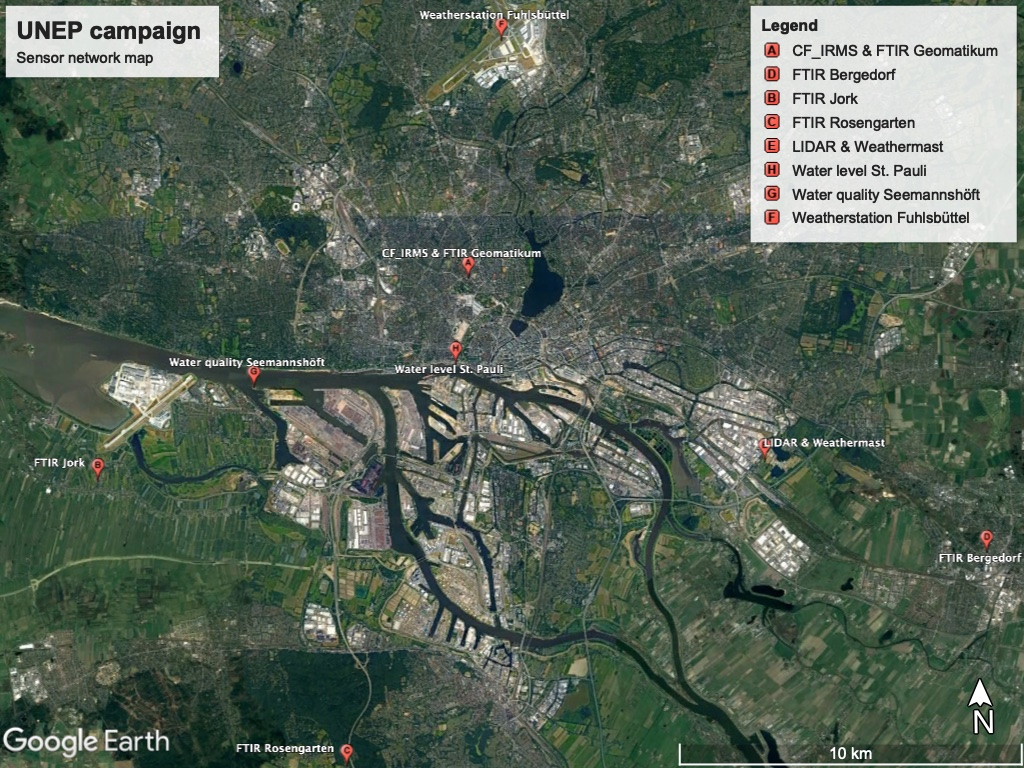
\includegraphics[width=1\textwidth]{figures/Appendix/Map/UNEP_map.jpg}
 \caption[UNEP Map of sensor network]{Satellite image of Hamburg with the location of the sensors deployed in the UNEP measurement campaign marked on the map. A: Geomatikum of University Hamburg with CF-IRMS, FTIR and Wind measurements, B: West FTIR station in Jork, C: South FTIR station in Rosengarten, D: East FTIR station in Bergedorf, E: Weather mast and Wind LIDAR both measuring wind in Billbrook, F: DWD Weather station Fuhlsbüttel, G: Water quality measurements at Seemennshöft, H: Water level measurements at St. Pauli. \cite{GoogleLLC.2023}}
 \label{UNEPmap}
\end{figure}
The enclosures operate by measuring the absorption infrared solar spectrum with a high temporal resolution of 90 seconds, which is later used in the retrieval process, averaged over a 10 min period to accurately calculate the CO$_2$, CH$_4$, and O$_2$ the column integrated dry air mole fractions. \\
The enclosures are equipped with a Michelson interferometer (Bruker, EM27/Sun). This spectrometer has an attached solar tracker that enables the tracking of the Sun by redirecting the light rays with a set of electronically controlled gold-plated mirrors. The spectrometer is housed in a weatherproof aluminium box to protect it and its auxiliary equipment, such as a computer, heating unit, control electronics, etc., from the elements. To enable an undisturbed light ray, the solar tracker sticks out the top of the box with an automatic cover that opens at favourable weather conditions and aligns itself with the solar tracker. To protect the tracker from precipitation, a rain sensor and a cloud detection sensor are placed on top of the enclosure. They automatically initiate a closure of the cover when precipitation is detected, or the cloud coverage is too great. The weatherproof enclosure and automated operation allow for autonomous data acquisition of a geographically extensive network with minimal staffing. Data collection during fluctuating weather conditions can be achieved as the measurement can be initiated and terminated quickly without lengthy setup times.
\begin{figure}[htbp]
 \centering
 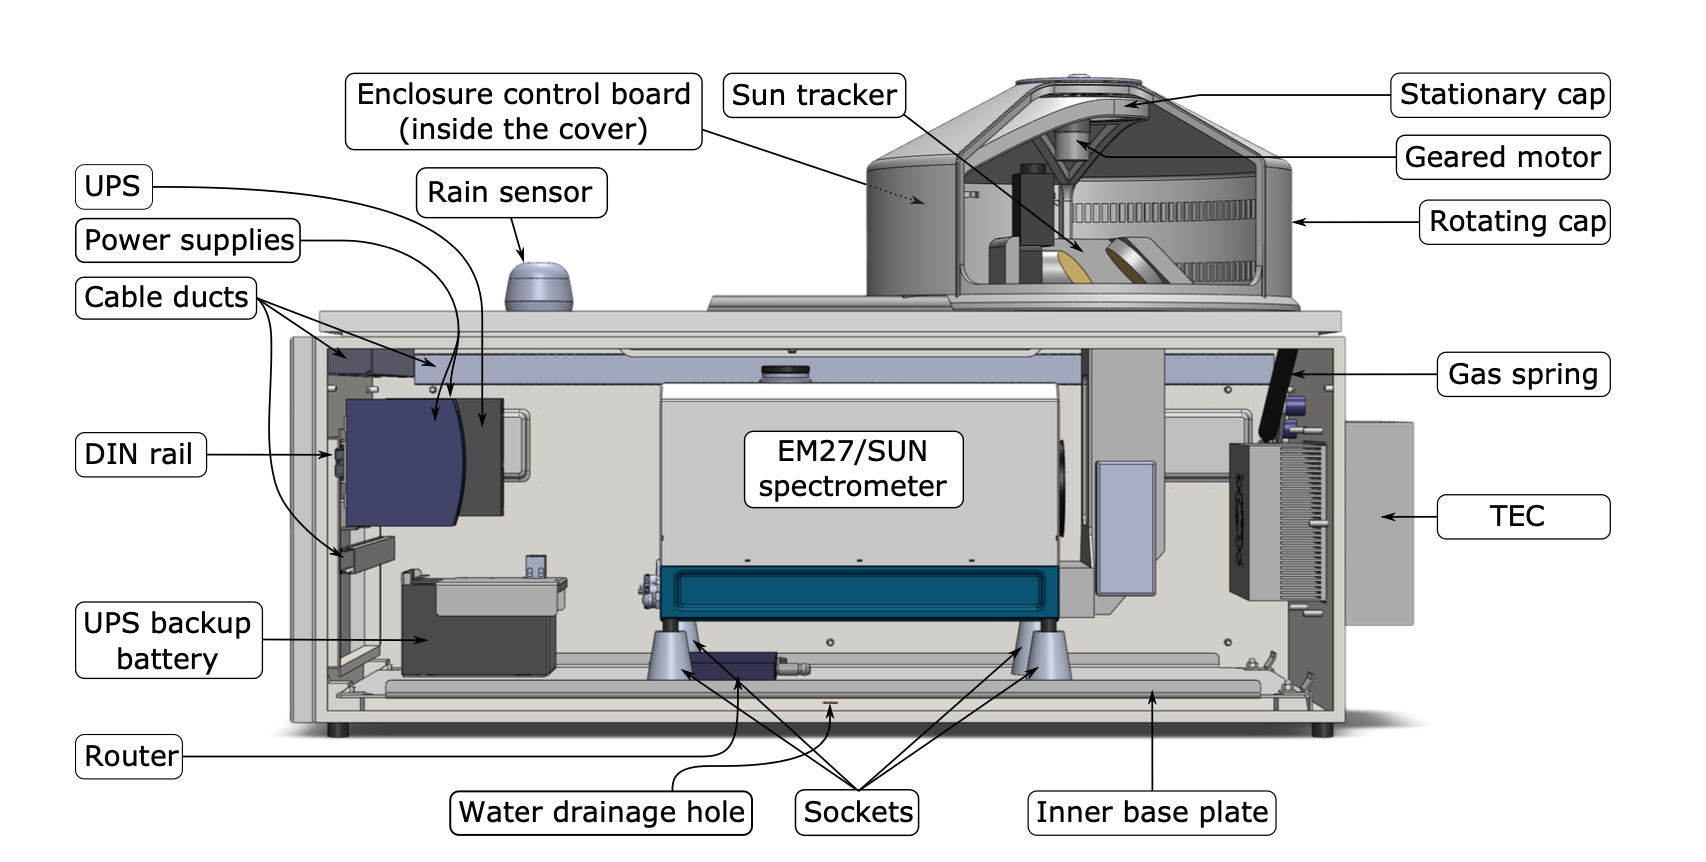
\includegraphics[width=1\textwidth]{figures/Methode/FTIR_Enclousure_schematics.png}
 \caption[FTIR spectrometer enclosure schematics]{Schematics of the FTIR spectrometer enclosure (MUCCnet). \cite{Heinle.2018}}
 \label{FTIRSchematics}
\end{figure}
The significant advantage of the FTIR approach to other in situ measurements lies in the total column measurement, which measures the total air column of the atmosphere between the light emitter, i.e. the sun and the spectrometer. The spectral absorption by the methane can then accurately be measured for the entire atmosphere. Other approaches that measure concentration at the street level have the disadvantage that they can miss methane emission emitted above the instruments like high chimneys. The degree of mixing of the GHG with the background air highly depends on various airflow characteristics, topography, emission type, and location. A total column measurement can’t negate all of them, but it gives a more reliable picture than simple in situ measurements. 

\subsection{Bayesian inversion modeling}
By using the FTIR sensor network,  differential total column measurements were performed, in which at least one sensor is always located upwind and one downwind of an emitter. The quantity of GHG released by an emitter can be estimated by comparing the concentration delta of the two columns.\\
A computational fluid dynamics (CFD) model is used to identify the emission location. This is aided by using a Bayesian inversion framework.\\
An inverse Framework is a method where the effects of an event or condition are used to calculate the cause that leads to the observed effects. Here the methane concentration was measured in the atmosphere, and it is attempted to calculate its emitters. In a forward method, the measured concentration in the air would be calculated from the known emitters.\\
To statistically improve the calculation of the cause, further prior information can be used. The TNO inventory, which has the highest spatial resolution of “known” emitters in Hamburg, is used in this case. This inventory is compiled by estimating emissions due to fossil fuel usage, density, type of emission, etc.
When applying the Bayesian approach in the Inversion, the TNO GHGco inventory was used as the prior estimation of the emissions.\\
The TNO GHGco Inventory is a European database with spatially resolved emission data for CO$_2$, CH$_4$, CO, NOx and NMVOCs. The spatial resolution is (1/60)◦ for longitude and (1/120)◦ for latitude” \cite{Super.2020} \cite{Super.2019}. This inventory is Hamburg's current highest resolution inventory, giving the best available prior emission estimation. Its limitation is that the Bottom-up approach may not encounter all emission sources or does not yet account for relocated and sporadic emitters. To further improve the inventory, an additional layer that contained estimated emissions from the Elbe was added. For this estimation of methane emissions from the separate sections of the Elbe by \cite{Matousu.2017} were added for each grid cell individually. Each grid cell was multiplied by the proportion of water coverage in this cell to account for the incomplete coverage of the Elbe by coarse raster \cite{Forstmaier.2023}.\\
In Bayes’s theorem, the posterior model is proportional to the prior model, which is the probability of the methane being emitted using previously acquired knowledge times the “likelihood of the Data”. The likelihood of the Data links the target model (the posterior of the measured variable) to the measured data. The likelihood is the probability of measuring a concentration given the emission from the Prior model.
\begin{equation}
Posterior probability = \frac{Prior probability * Likelihood of the data}{Normalization constant}
\end{equation}
\begin{equation}
P(A|B) = \frac{P(B|A)P(A)}{P(B)}
\end{equation}
A Bayesian inversion can estimate the methane emission of a source by using prior knowledge of the source by updating this knowledge with measurements of the methane concentration in the air.\\
To identify the locations, the Inversion also uses the ERA5 weather model. This model is additionally corrected for the boundary layer height and wind direction using a wind LIDAR. This corrected model is then used to generate backward trajectory footprints with a Stochastic Time-Inverted Lagrangian Transport (STILT) model. The Inversion is then able to use the STILT footprints for its identification of the emission location. For the UNEP campaign, the existing framework developed by \cite{Jones.2021} was adopted for Hamburg and used in the analysis.

\section{Peak identification algorithm}
The Isotope ratio mass spectrometer measurements show a series of methane concentration peaks throughout the campaign time, with different magnitudes and durations. Hence the identification and characterisation of the peaks were of great importance. To achieve this goal, a peak finder algorithm was implemented that identifies the methane peaks over the entire time series. Outputting the maximal concentration and its time, together with the peaks start and end time and concentrations. The peak finding algorithm was tuneable in its identification criteria, allowing for separate investigations. With the peak identification, an automated tool was provided to be used later in the pipeline for isotope signature identification and correlation with other variables.\\
In the analysis, two different identification criteria were consequently used. The first was the identification of all methane peaks that are distinct from the background concentration. The identification criteria defined by \cite{Menoud.2021} were used as a reference. The following criteria were applied:
\begin{itemize}
  \item A minimum enhancement above the background of 100 ppb.
  \item A minimum peak height of the lowest 10th percentile of the concentration-time series.
  \item The peak width contains at least 3 data points (approximately 60min).
  \item The peak width is restricted to maximum ± 6 hours around the centre of the peak.
\end{itemize}
Figure \cref{TimelinePeaksPaper} shows an example of the peaks with the identified peak highlighted.\\
The second peak identification criteria are designed to identify only the short and very prominent peaks. Those peaks are visually different from most others, and a different production mechanism was suspected. The peculiarity of those peaks was separately investigated to identify the mechanisms that govern those peaks. The criteria applied are as follows:
\begin{itemize}
  \item High concentration of min 2100 ppb.
  \item Min 3 data points.
  \item Shorter max peak spared of 3 h.
\end{itemize}
An example of the identified peaks can be seen in \cref{TimelineMediumPeaks}. 

\section{Methane and environmental data correlation analysis}
\subsection{Methane emissions with water level}
At first inspection, the presence of the methane peaks in the concentration timeline occurs at random. Overlaying the methane concentration with the water level measurements at St. Pauli in Hamburg, provided by Bundesanstalt für Gewässerkunde (BfG), indicates a correlation.
A pattern can be spotted in Figure Plot \cref{TimelineCH4Waterlevel}, which is a section of the complete timeline. The dominant methane peaks occur around 1-3 h after the lowest water level. \\
While smaller peaks are visually more challenging to identify and correlate to the Water level, the peak identification algorithm helps to highlight the smaller peaks. It further indicates a correlation with the water level of the river Elbe. \\
Pearson's correlation coefficient was used to prove a statistically meaningful correlation between the water level and the methane concentration. Unfortunately, the occurrence of elevated methane concentrations doesn’t seem to be a single variable correlation. So, a simple correlation of the total water level and concentration yields no correlation. \\
The wind direction must be considered to establish a correlation between water level and methane. This was done by separating the timeline in wind directions and speeds to be analysed separately by binning all methane and water level measurements in 10° Wind directions and 1 m/s wind speed bins. Followed by calculating the Pearson's correlation coefficient between the water level and methane concentration in the air for each bin.\\
A visual representation of the obtained results can be seen in Plot \cref{WaterLevelPCCGeomatikum}. Each tile in this plot represents a wind data bin, with the colour representing Pearson's correlation coefficient.\\
It can be seen that in three regions with particular directions and speeds, a strong correlation between methane and the water level is observed.\\
To validate if the correlations are statistically meaningful, a p-value test has also been conducted with a value of $<$0.05. A plot visualizing the results can be seen in \cref{WaterLevelCorrPValueGeomatikum}.\\
Fortunately, the Regions of interest pass the test, while the regions that don’t show a correlation to the water level fail the test as expected.

\subsection{Methane concentration and water quality correlation}
It is well known that wetlands and waterbodies can release significant amounts of methane into the atmosphere. \cite{Matousu.2019} show that a high methane concentration in the water of the Elbe is present in the upper estuary of the city of Hamburg. The TNO GHGco inventory does not include emissions from the river Elbe, but \cite{Forstmaier.2023} shows that a correction including estimations of the river's emissions yields more reliable modelling results.\\
Water quality parameters are a good indicator of methane production, reduction and emission rates in the water \cite{Wu.2007}.  A direct methane emission prediction cannot be made just from such water quality parameters due to the complexity of the production mechanism and its strong dependence on local conditions and microbial composition present in the water body. Nether the less, a correlation between water quality parameters and methane production was observed. This can help to provide further indication of alleviated methane concentration in the air due to mechanisms in the water of the river Elbe. \\
To investigate if the methane peaks and the methane concentration in the air are connected to the river Elbe, the water quality parameters of the Elbe have been correlated with the methane concentration time series.\\
The water quality data measured at Elbe Seemannshöft provided by Hamburg Service were used \cite{IHUW.20230501}. This data included the parameters: Water temperature, Oxygen concentration and saturation, pH-value, conductivity $\kappa$25, turbidity, UV-absorption SAK and algae concentration of different types. The data had a high temporal resolution of 10 min. \\
A Pearson's correlation coefficient analysis was made using the same correlation approach described before for the same wind direction and speed bins. An example can be seen in \cref{CorrelationWaterQuality}.

\subsection{Methane concentration and meteorological observations correlation.}
The release of methane into the atmosphere by natural and anthropogenic mechanisms is highly dependent on environmental conditions. These include, for example, meteorological parameters such as temperature, precipitation, and solar intensity.\\
For natural methane emissions, methane production and release into the atmosphere depend highly on temperature. Different microbes have a preferred temperature at which their methane production or reduction mechanisms peak. Higher temperatures are generally favourable for methane production \cite{Singh.2000}. Another significant parameter is the precipitation amount and consequent water abundance on the surface. Some microbes live in water or moist environments. An abundance of surface water aids the population growth of such microbes. Additionally, water can help to flush organic material into the waterbody providing a plethora of nutrition for the microbes, allowing for a large population and methane production. \\
Anthropogenic methane production is differently affected by meteorological parameters as the behaviour of humans mainly governs it. A well-observed example is the increase in fossil fuel consumption at colder temperatures \cite{Javadinejad.2019}. This is primarily observed in an annual cycle. Methane from anthropogenic sources is often released into the atmosphere through leaks in the infrastructure or incomplete combustion. Other parameters and mechanisms also exist and are primarily dependent on the environment.\\
It was attempted to investigate a possible correlation between the methane concentration in the air and some meteorological parameters.  The Deutsche Wetteredienst (DWD) data was used for this. The measurement station Hamburg-Fuhlsbüttel was used due to its proximity to the Geomatikum (2.3 km). This Station provides highly standardised and quality-controlled measurement data, which were 10 min and 1 h averaged by the DWD \cite{Kaspar.2013}.\\
The measurement parameters investigated were: air temperature at 2 m, dew point, humidity, precipitation, air pressure, and solar radiation intensity.\\
The correlation investigation was performed in a similar manner as with the water quality and water level. A Pearson's correlation coefficient analysis and a P-value test for separate wind direction and speed bins, the resulting correlations were plotted in a tile plot for better visualisation.

\section{Methane transport by wind}
\subsection{Methane emissions and wind measurements}
As previously mentioned, the wind plays a significant role in the measured methane concentration at the Geomatikum. Hence a detailed analysis of the observed wind is essential. The wind data from the Deutsche Wetterdienst (DWD) and Universität Hamburg was used in this thesis. \\
The Deutscher Wetterdienst (DWD) provides weather and climate data throw their Open Data Climate program \cite{DeutschenWetterdienst.20230501}, with an extensive array of measured parameters at different measurement time intervals for a large selection of weather stations. In Hamburg alone, there are two Stations and about five near the city. In this thesis, the data from the Fuhlsbüttel, Hamburg Station, has been used due to the proximity to the Geomatikum, where the CR-IRMS and one of the FTIR spectrometer stations were located. \\
A significant advantage of using the data provided by the DWD is the standardization and quality control done by the DWD, providing considerable confidence in the measurements. Additionally, the wide arrange of measured parameters provided, including, for example, precipitation, soil and air temperature, solar radiation intensity, etc., enables comparison and correlation with many aspects of methane emission.\\
While this data adheres to strict standards, the wind measurements are performed only 2 m above ground. Measurements of this altitude are heavily influenced by surrounding topography. While time averaging helps in normalising the measurement, it does impact the temporal resolution of the measurements.\\
The Universität Hamburg provided three different sets of wind measurements at two locations \cite{Lange.20220501}. The first location was at the Geomatikum itself, only a few metres from the CF-IRMS measurement inlet at the height of 83 m. At this height, the surface-level effects are mostly negated. But the Geomatikum building itself can potentially generate turbulences that influence the measurements. The Geomatikum was the highest building in the proximity by quite a margin, but disturbances from the surrounding can’t be completely out-ruled. The second location is at the weather mast in Hamburg Billbrook, about 17.3 km East of the Geomatikum. Measurements there were made at the height of 50m and 110m. The measurement instruments are placed far from the support structure so that disturbances by the mast are minimised. Additionally, no high-rise buildings are located near the mast, aiding a mostly undisturbed measurement.\\
All four measurement data sets were time averaged over 10 min, and all were analysed and used in further modelling. The measurements at the Geomatikum proved to be the most reliable data set, and the analysis in this thesis mainly focuses on it. The proximity to the isotope measurement inlet was the main contributor to the reliability, as small local wind patterns were picked up by both measurements simultaneously. 

\subsection{Methane emission distance modelling}
In the methane concentration time series at the Geomatikum, the prominent peaks are very sharp, with a relatively short duration of 0.5 to 3 h and a very high methane concentration of up to 4000 ppb for a background concentration of 2000 ppb. This indicates an emitter located nearby with a relatively short emission time and a high amount of methane released. \\
To estimate the Distance between the emitter and the measurement location,
the strong correlation between the methane concentration in the air and the tidal cycle of the Elbe is used.
To achieve this, virtual tracks of wind particles are modelled using the wind data measured at the Geomatikum. \\
%check and rewrite the Elipsodial disatance formular plus add reference
The tracks are modelled for the time between the maximal methane concentration of a peak and the lowest water level during the low water cycle of the Elbe before the methane peak. Tracks are backwards-modelled in time, originating at the Geomatikum. The particle follows the measured wind, with a time resolution of 10 min as dictated by the measurement. At each 10 min interval, the partial location is calculated using its previous location, the wind data and Bowring's Ellipsoidal-surface formulae.  This is repeated until the time when the lowest water level is reached. The total 
Geodesics distance between the Geomatikum and the final location, i.e. the estimated emission location, is then calculated. The resulting distance for all peaks is plotted versus its peak's maximal methane concentration in a scatterplot. This can be seen in \cref{DistancePlot}.

\subsection{Gaussian plume transport modelling for methane peaks}
A transport model was constructed to locate the emission regions causing the prominent methane peaks. For this purpose, the temporally high-resolution wind data provided by the University of Hamburg and the Deutsche Wetterdienst (DWD) have been used. The transport model uses the wind data to create Gaussian plumes with the measurement site as a particle emitter.\\
The emitted particles travel backwards in time; this allows the calculation of reversed particle tracks. To create Gaussian plumes at a specific emission time, many particles are emitted simultaneously at this time. The particle tracks are calculated using the wind direction and speed for each wind measurement interval. So that the particle can follow changes in wind direction and speed over time. The direction and speed of each particle are randomised with a predetermined Standard deviation at each interval for each particle. The degree of randomisation was taken from literature values for similar topography and wind speeds as in Hamburg (SD wind speed 0.5 m/s, SD wind direction = 20° \cite{Farrugia.2017}). The standard deviation was calculated for each wind measurement dataset using the rolling Yamartino method for the wind direction and a normal standard deviation for the wind speed showed similar values for all datasets. As a large number of particles are emitted, the randomisation on each individual particle yields a Gaussian distribution for the total particle distribution.\\
The transport model was used in tandem with the peak finding algorithm to investigate the peak methane emission locations. After the methane peaks are identified, the time of lowest water level is within 12 h before the methane peak is identified. 
Around half an hour before the lowest water level, the majority of the shallow water regions of the Elbe are completely water-free, exposing the soil and sediments to the air. Those regions can be seen in \cref{TopographyElbeHamburg}, showing a topographic map of the Elbe  in Hamburg. The Regions that dry out during a low tide start from 0m (yellow) to 2.7 m (red). It has to be noted that this survey does not include all connected channels and Fleeds surrounding the Elbe. Most are located in and around the city centre, and all of them are exposed during low tide. To account for all the sections of the river that dry out before the lowest water level is attained, Half an hour before the lowest water level is calculated. It is estimated that at this time, the majority of the shallow regions are dry, but due to the change in the tidal range over a lunar cycle, this can vary substantially.
\begin{figure}[htbp]
 \centering
 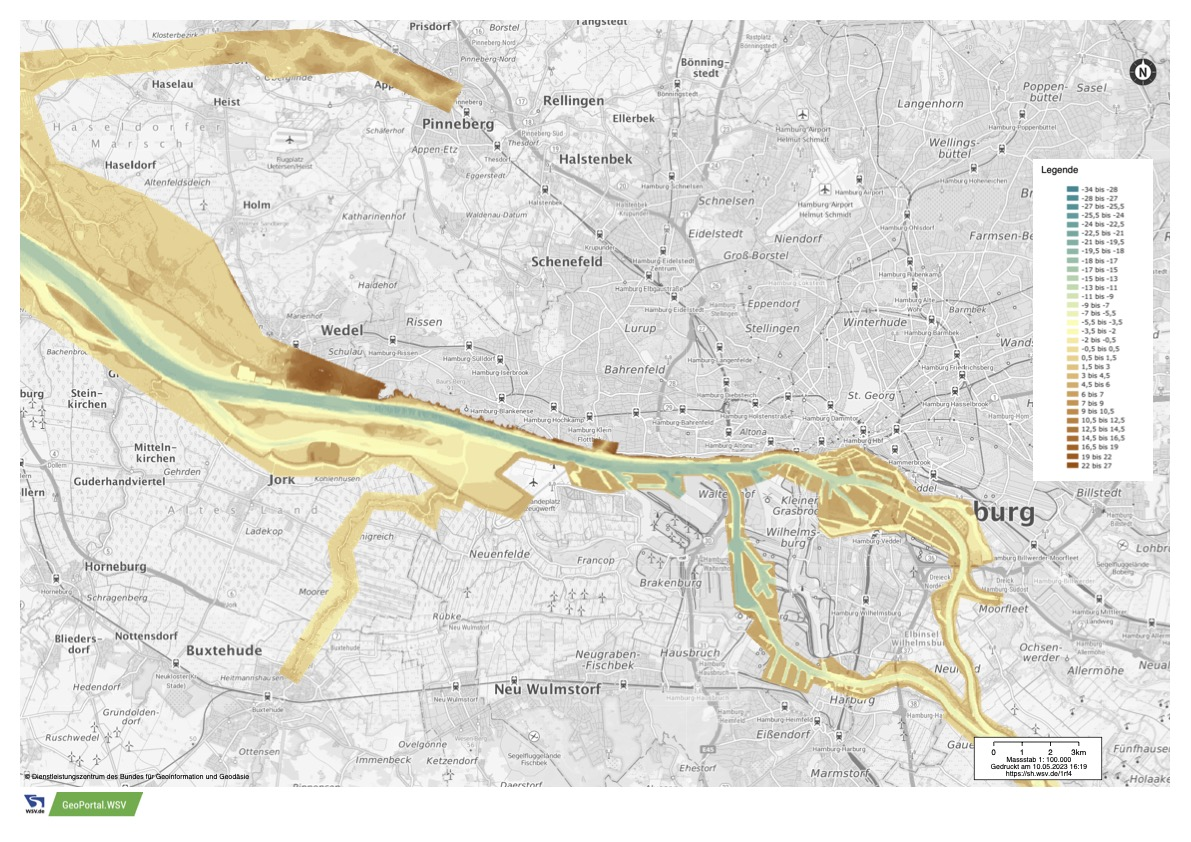
\includegraphics[width=1\textwidth]{figures/Appendix/Map/TopographieElbeHamburg.jpg}
 \caption[Topographic map of Elbe in Hamburg]{Topographic map of the river Elbe in the Hamburg region, Scale is in dm, 0 dm is at mean sea level. \cite{ZDMGDWS.2016}}
 \label{TopographyElbeHamburg}
\end{figure}
The particle tracks are only calculated for the time between this half hour before the lowest water level and the maximum methane peak. \\
After all particle tracks for all selected emission times are completed, the particle distribution density is calculated. This is done by splitting the map into a 1000x1000 segment raster and calculating the density of particles in each segment. The raster is then normalised for the total domain. The transport model outputs a map with the rasterised particle density overlay as an interactive map \cref{TransportmodelStrictPeaks}.\\
Using this approach, it can be observed that many particle tracks follow the path of the  Elbe quite closely. 


\chapter{Results}
\label{chap:Results}

\section{Methane peaks}
With the aid of the methane peak identification tool, the peaks were investigated in detail. In \cref{TimelinePeaksPaper} and \cref{TimelineMediumPeaks}, a small segment of the total concentration timeline can be seen.
\begin{figure}[htbp]
 \centering
 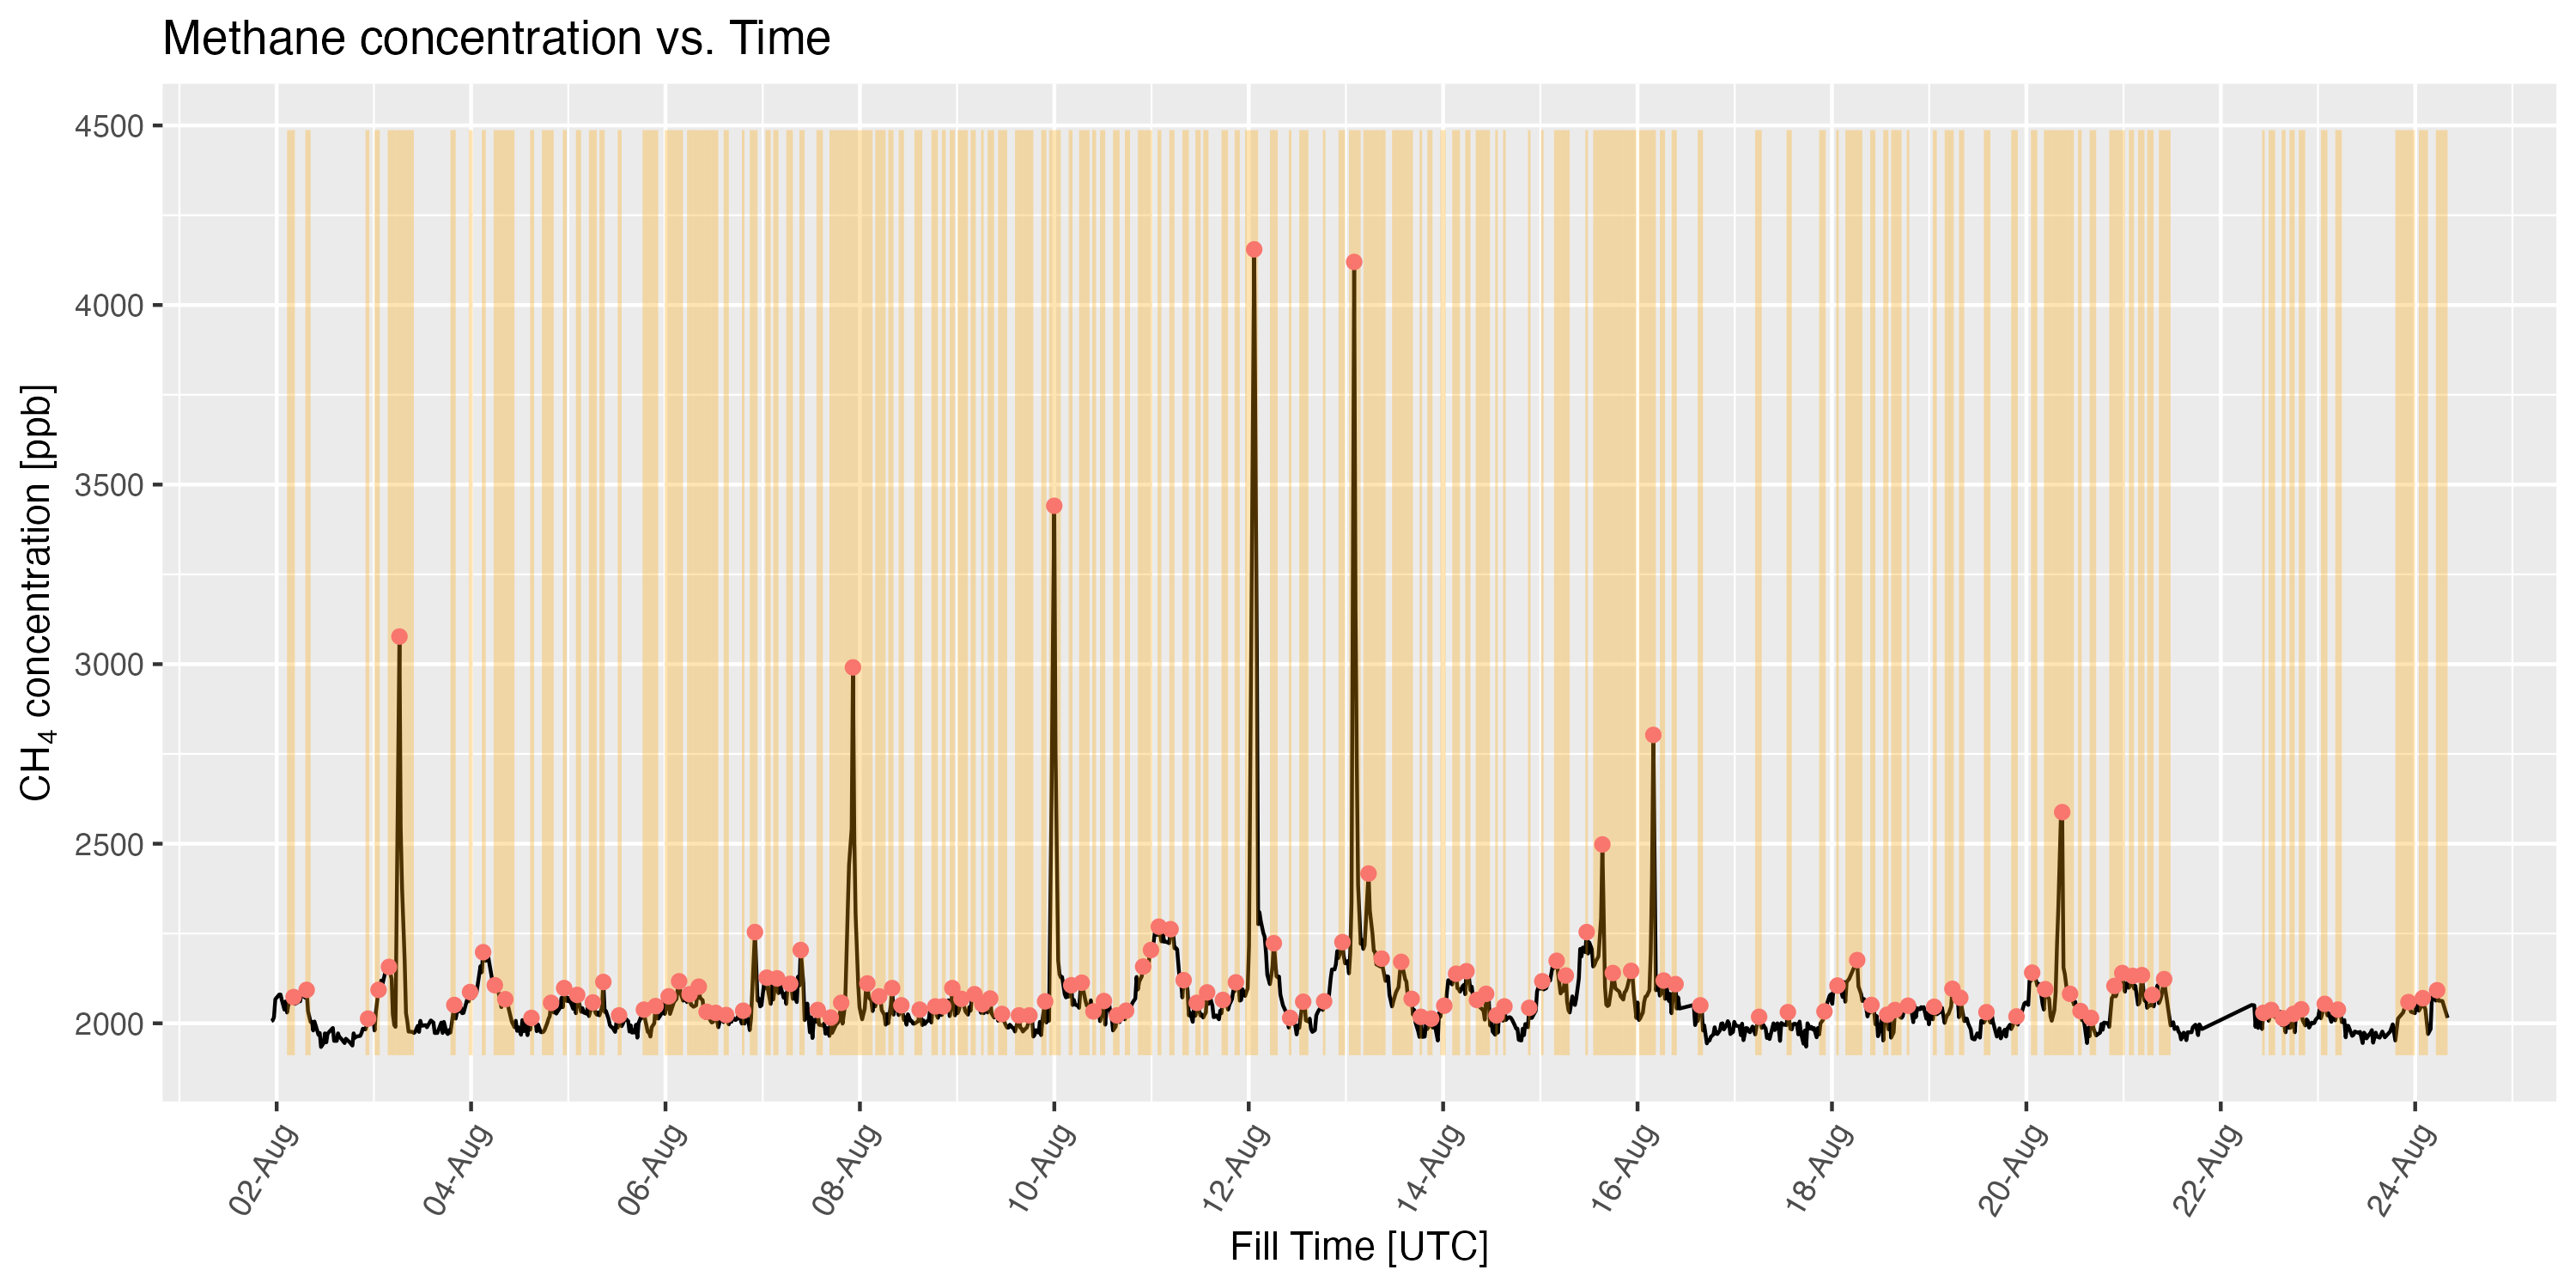
\includegraphics[width=1\textwidth]{figures/Appendix/CH4_Timelines/4_CH4_Timeline0_Paper_Peaks.png}
 \caption[CH$_4$ Timeline with peak identification from literature]{Section of CF-IRMS measurement showing the timeline of methane concentrations measured in Hamburg Geomatikum (83m above ground) from 02.08.2021 to 24.08.2021. Peak identification criteria by \cite{Menoud.2021}. The red dot indicates the peak centre and the orange section highlights the peak width.}
 \label{TimelinePeaksPaper}
\end{figure}
\begin{figure}[htbp]
 \centering
 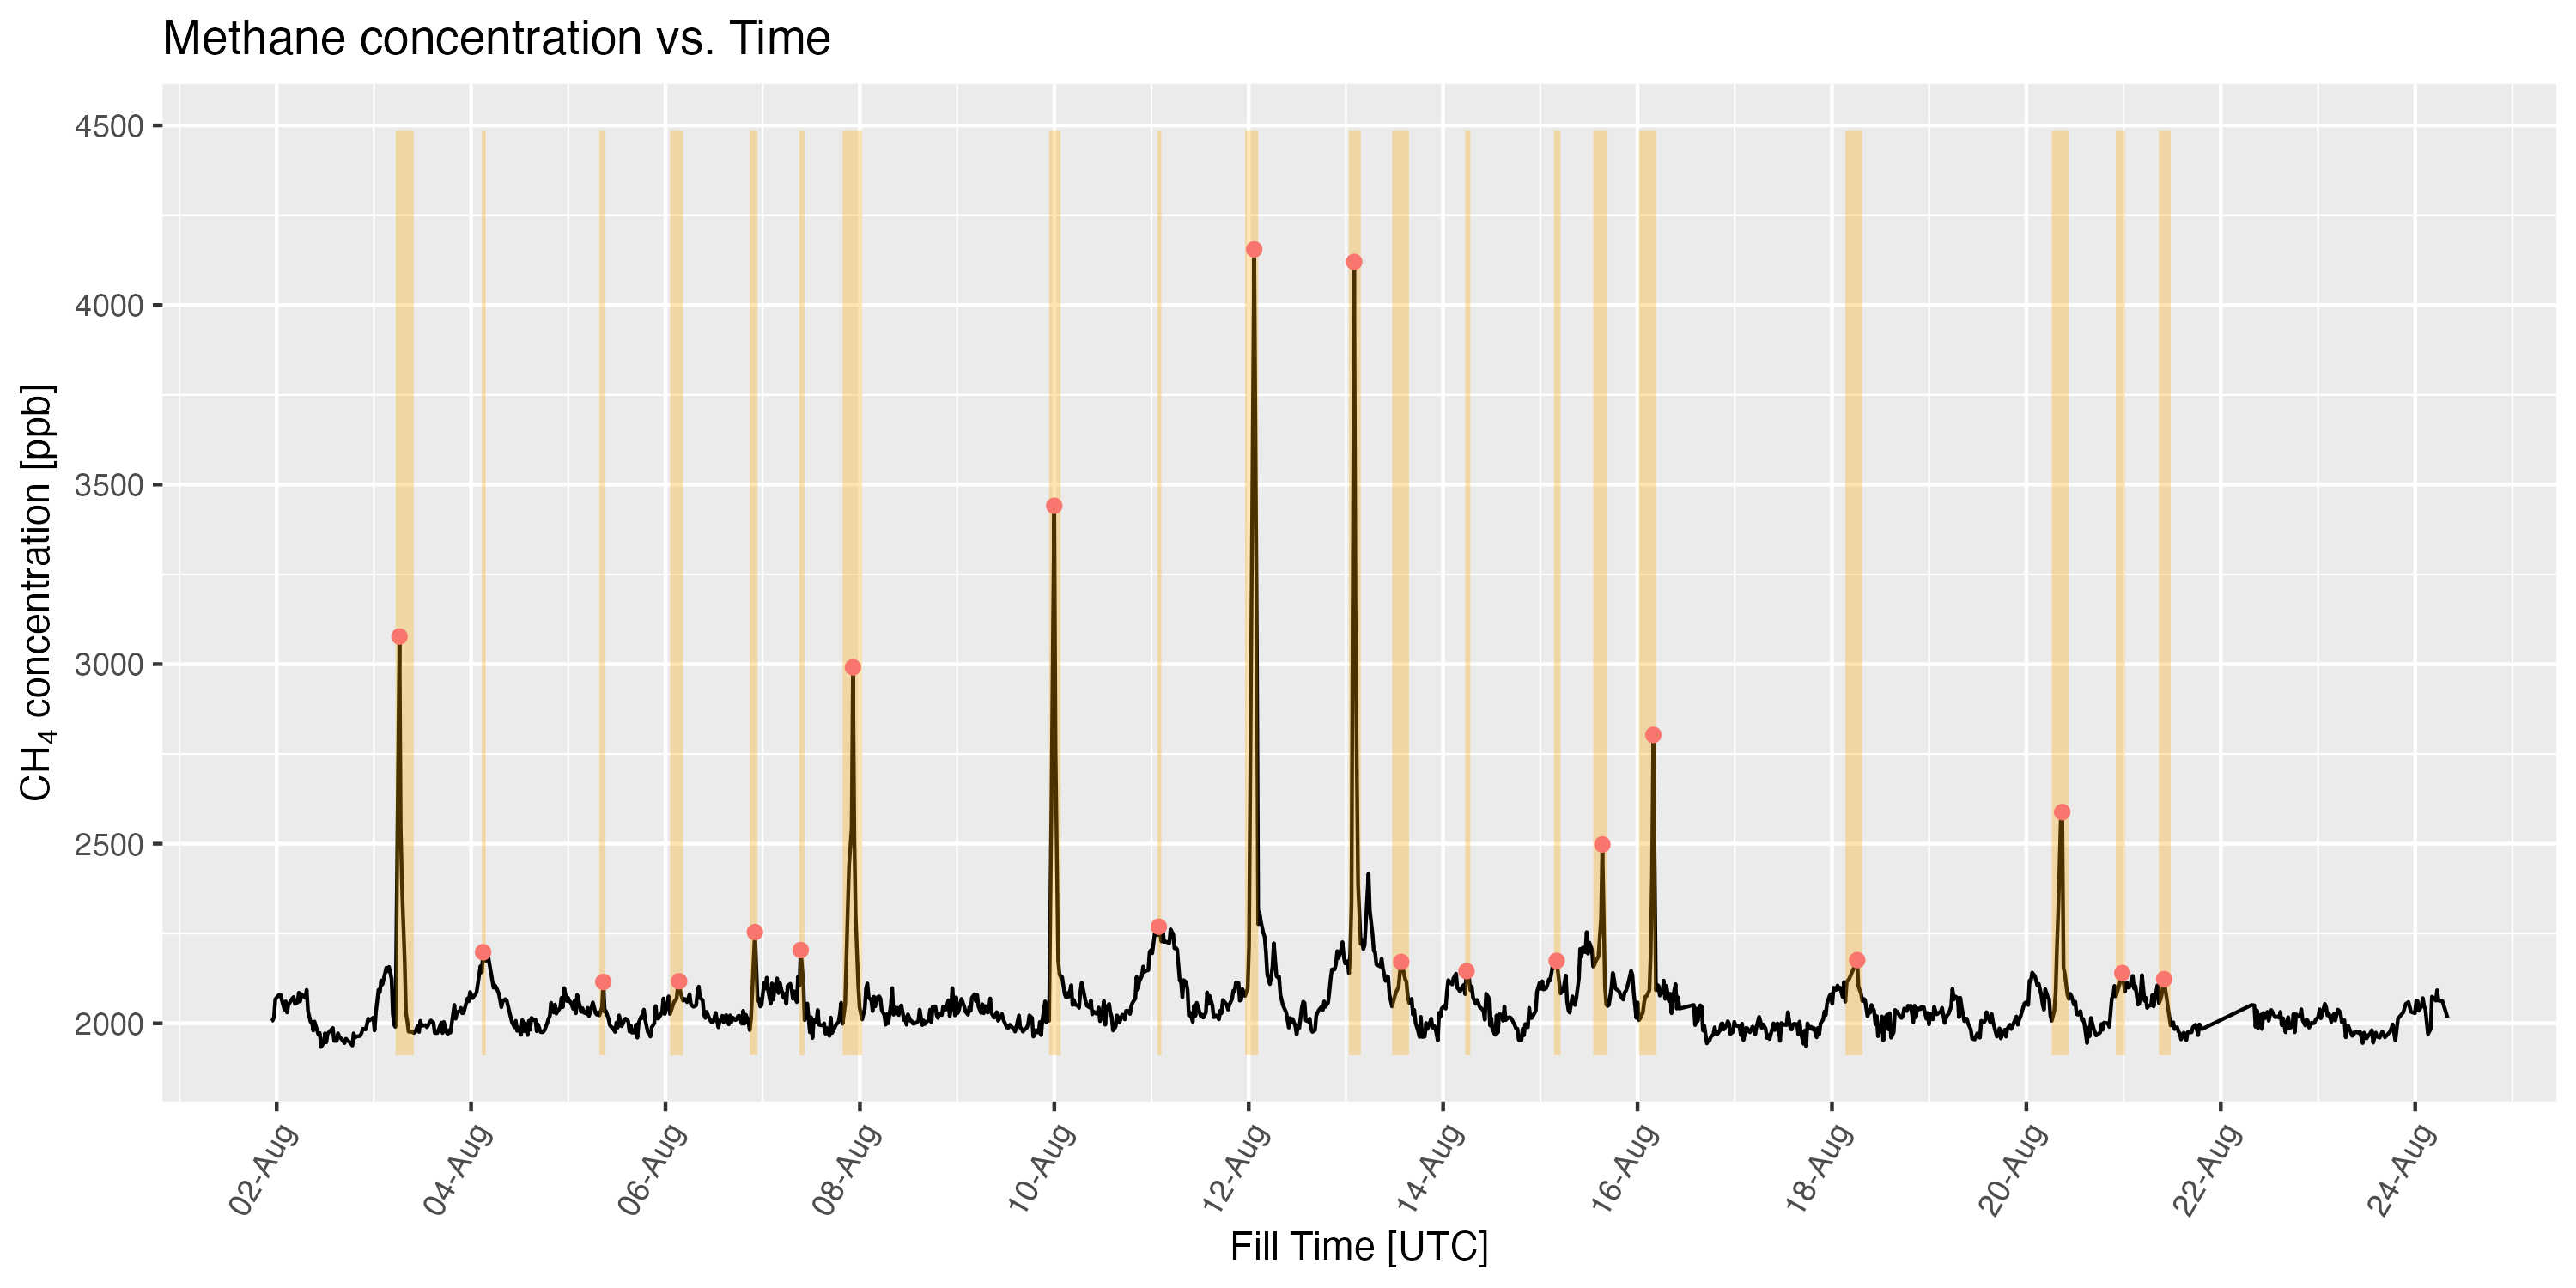
\includegraphics[width=1\textwidth]{figures/Appendix/CH4_Timelines/4_CH4_Timeline0_Medium_Peaks.png}
 \caption[CH$_4$ Timeline with strict peak identification]{Section of CF-IRMS measurements showing the timeline of methane concentrations measured in Hamburg Geomatikum (83m above ground) from 02.08.2021 to 24.08.2021. Peak identification criteria are chosen for only prominent peaks. The red dot indicates the peak centre and the orange section highlights the peak width.}
 \label{TimelineMediumPeaks}
\end{figure}
Nearly all peaks are accounted for in the first image, where the peaks are selected according to literature criteria. The smaller peaks occur at a relatively high frequency with a substantial irregularity. The number of peaks per day varies between 5 to 15 peaks. While during warmer months, August, September and October, the frequency of the peaks is lower than for the colder month, December, January, and February, see \cref{PeakHistogramm}.
\begin{table}[h!]
\centering
\begin{tabular}{||c c c c c c c c c||} 
 \hline
 & Aug. & Sep. & Oct. & Nov. & Dec. & Jan. & Feb. & Mar. \\ [0.5ex] 
 \hline\hline
  A: & 164 & 182 & 195 & 185 & 205 & 174 & 145 & 190 \\
  B: & 23 & 31 & 37 & 32 & 36 & 28 & 20 & 23 \\ [1ex] 
 \hline
\end{tabular}
\caption[Methane peaks per moth table]{Table of methane peaks per month using two different identification criteria. A: Selection criteria by \cite{Menoud.2021}. B: Strict criteria only selecting prominent peaks}
\label{PeakHistogramm}
\end{table}
Intermediate and prominent peaks occur at relatively regular intervals, while there are never more than two peaks within a day, and their peak centres are never closer than 12 h apart. \\
In the second image, the identification criteria are purposely designed to identify the prominent large and intermediate peaks and highlight the peaks well. Those peaks occur during the entire measurement campaign but with a higher frequency and concentration during the warmer months than the colder ones. The peaks are all quite sharp, i.e., with a short duration and high concentration compared to the background.

\section{Methane correlation analysis}
\subsection{Elbe water level methane correlation} \label{MethaneWaterLevel}
When the methane concentration timeline is overlayed with the water level of the Elbe, see \cref{TimelineCH4Waterlevel}, it can be seen that the prominent methane peak occurs shortly after the low water of the river. This behaviour is observed throughout the measurement period. The peaks occur, on average, 2$\pm$1 h after the low water.
\begin{figure}[htbp]
 \centering
 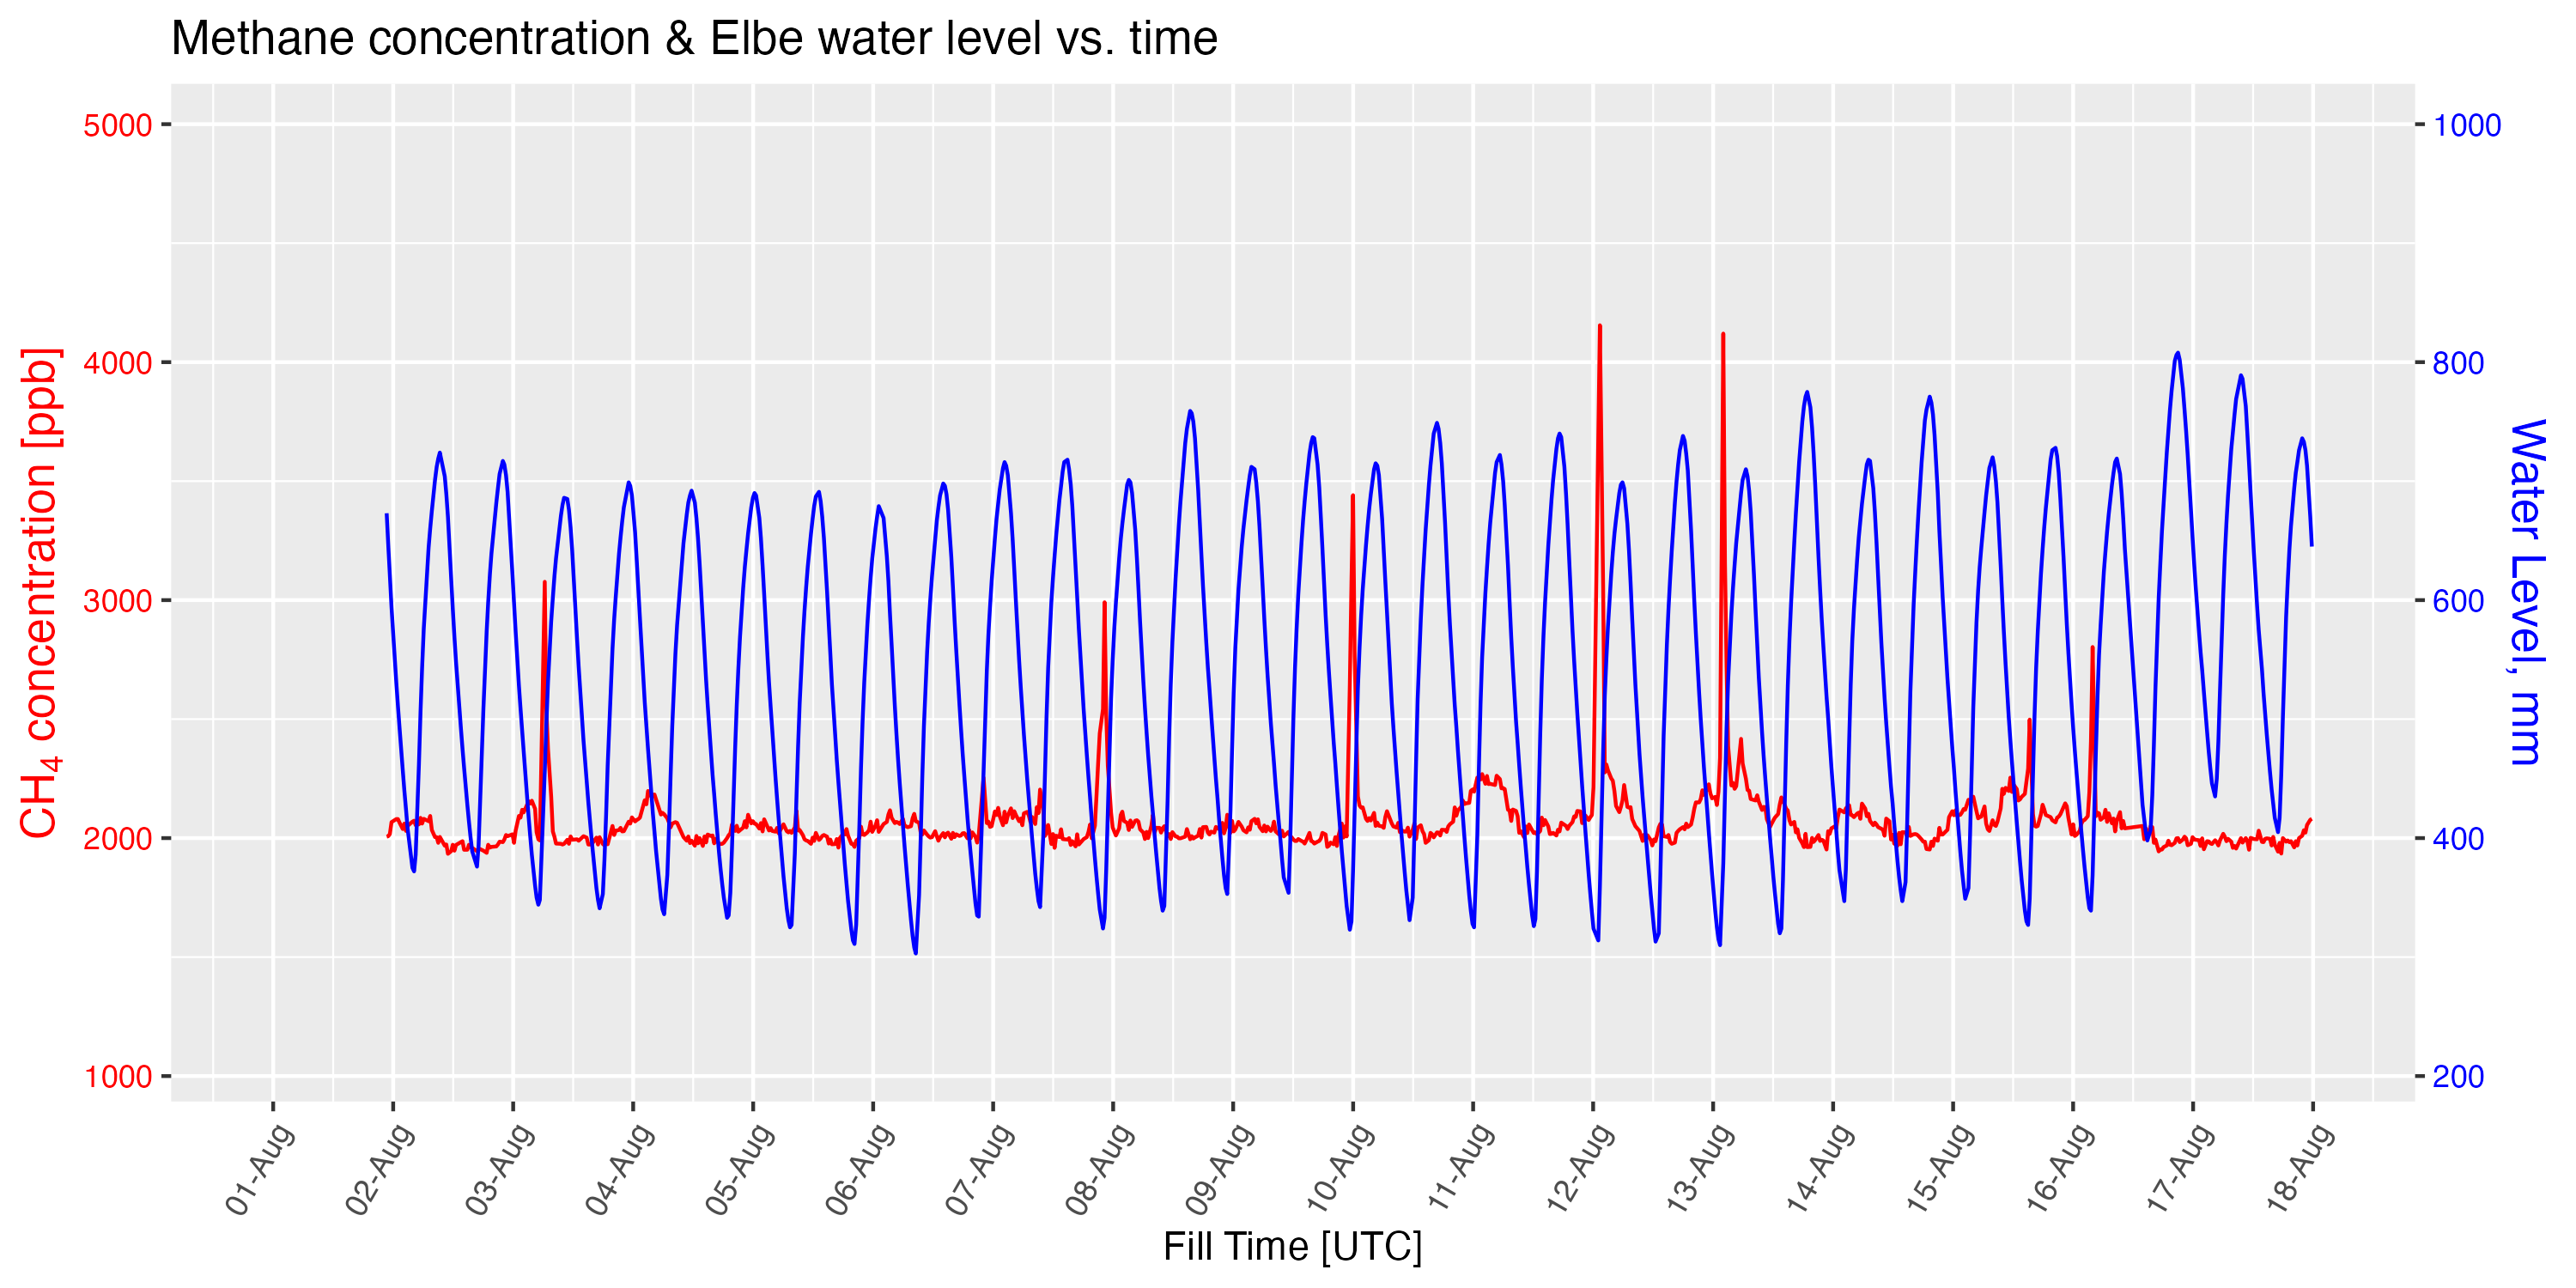
\includegraphics[width=1\textwidth]{figures/Appendix/Water_Level/1_CH4_WL.png}
 \caption[CH$_4$ Timeline with Elbe Water level Overlay]{Section of the CH$_4$ concentration timeline measured with the CF-IRMS at the Geomatikum (Red). Overlayed by the water level timeline of the river Elbe (blue). Measurements from 02.08.2021 to 18.08.2021 are shown.}
 \label{TimelineCH4Waterlevel}
\end{figure}
As the prominent methane peaks can’t be observed during every low water cycle of the river, additional factors seem to contribute to their production. But to establish a statistically meaningful correlation, Pearson's correlation coefficient between the water level and the methane concentration was investigated as previously described.
This correlation can be seen in  \cref{WaterLevelPCCGeomatikum}. Here, the measurements are binned by speed and direction using the Wind measurements made at the Geomatikum.
\begin{figure}
\centering
\begin{subfigure}[b]{1\textwidth}
   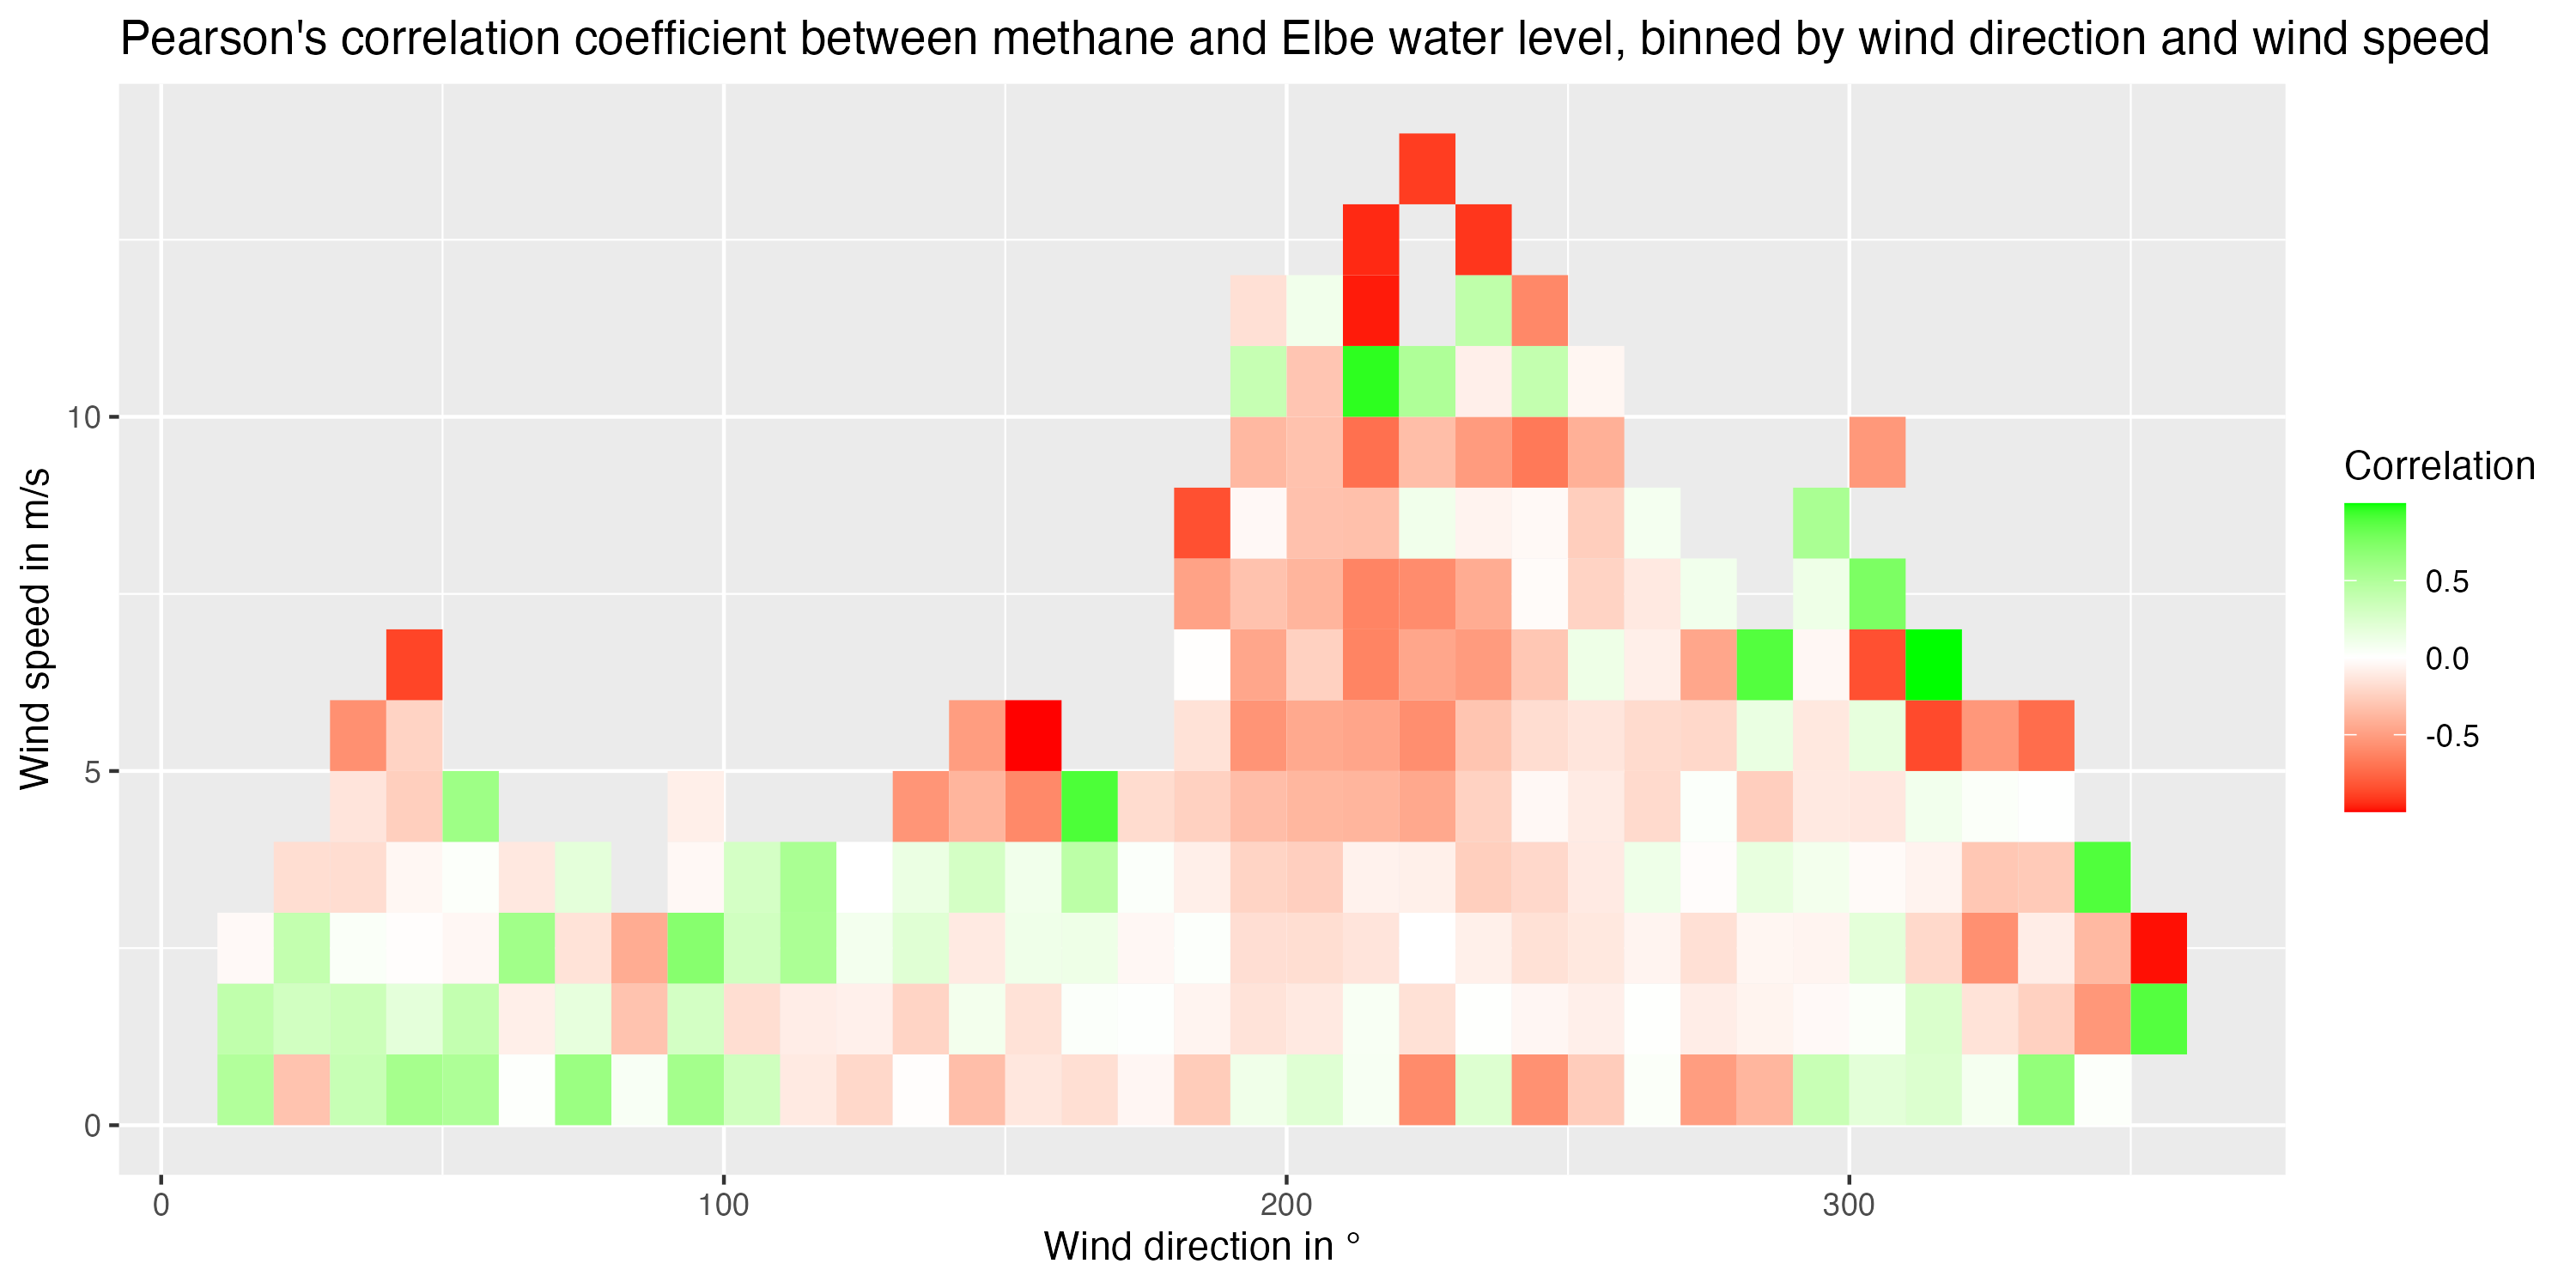
\includegraphics[width=1\linewidth]{figures/Appendix/Water_Level/13_CH4_vs_Waterlevel_Correlation_Geomatikum.png}
   \caption{}
   \label{WaterLevelPCCGeomatikum} 
\end{subfigure}
\begin{subfigure}[b]{1\textwidth}
   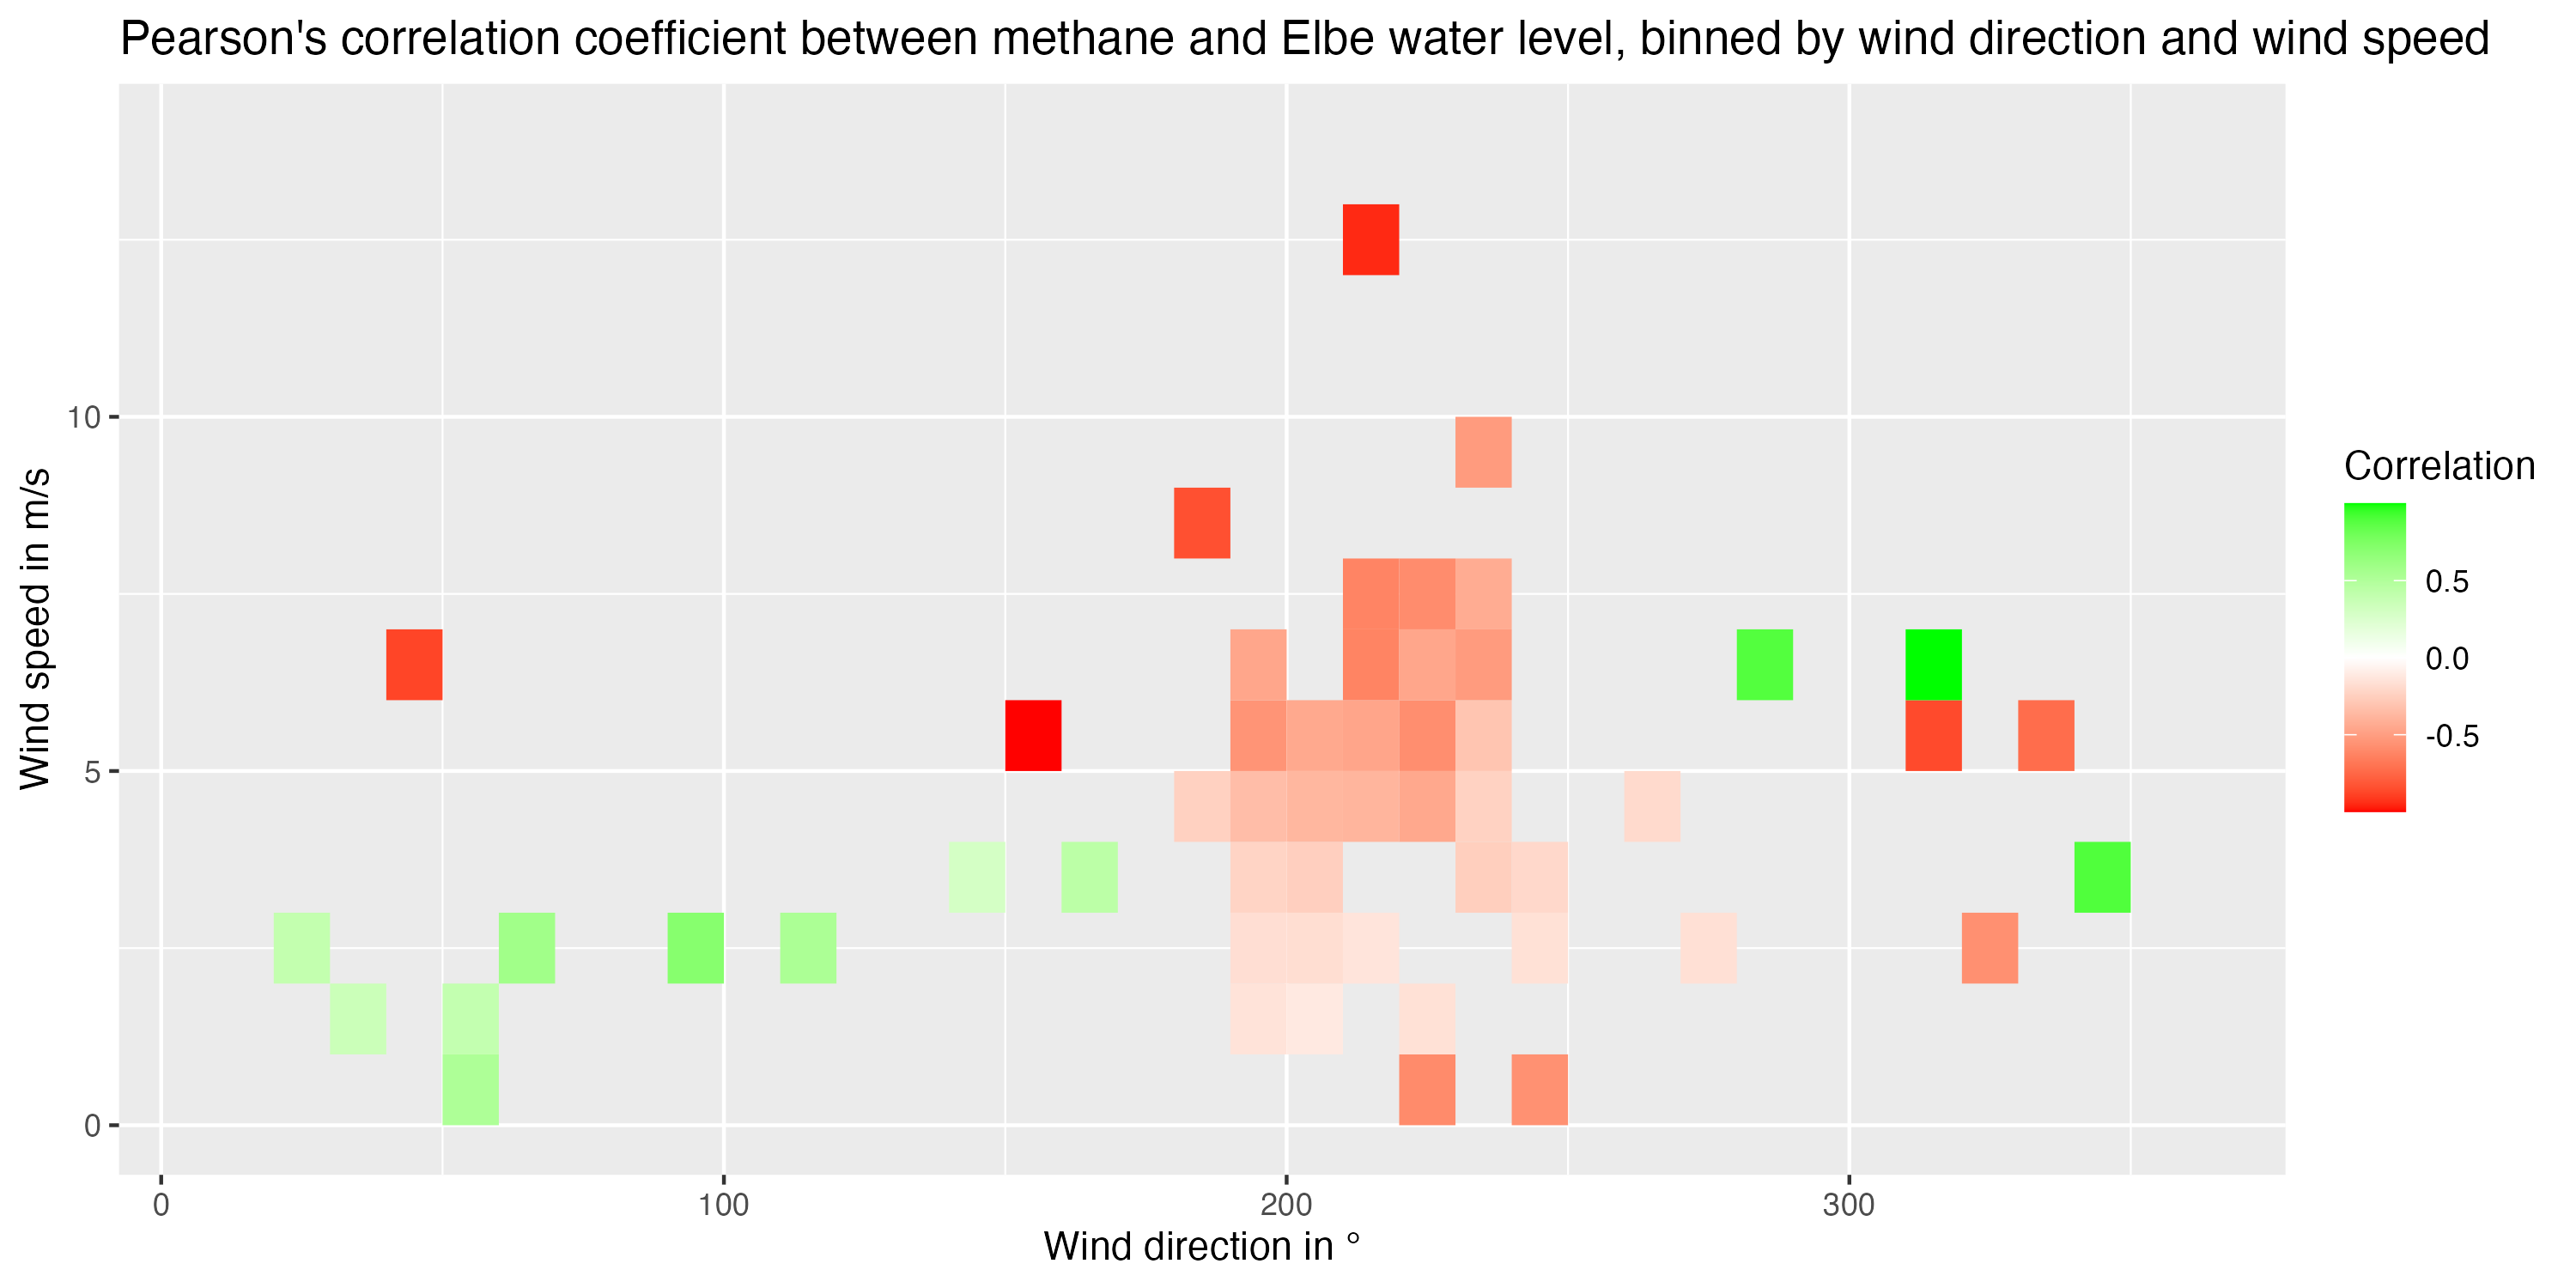
\includegraphics[width=1\linewidth]{figures/Appendix/Water_Level/13_CH4_vs_Waterlevel_Correlation_P_value_Geomatikum.png}
   \caption{}
   \label{WaterLevelCorrPValueGeomatikum}
\end{subfigure}
\caption[Correlation between CH$_4$ and Water level]{(a) Pearson's correlation coefficient between methane and Elbe water level, binned by wind direction and wind speed. Green shows a positive correlation (enhanced CH$_4$ at high water level), and Red shows a negative correlation (enhanced CH$_4$ at low water level). (b) Shows only the correlations which pass the 5\% P-value test for methane and Elbe water level, binned by wind direction and wind speed.}
\label{WaterLevelCorrelationGeomatikum}
\end{figure}
The plot shows a positive correlation with a green colour and a negative correlation with a red colour. A positive correlation indicates an elevated methane concentration in the air with a high water level of the Elbe. In contrast, a negative correlation indicates a correlation between methane concentration in the air with a low water level of the Elbe. The P-value test in \cref{WaterLevelCorrPValueGeomatikum} checks if the correlation is statistically meaningful. If the P-value is $<$0.05 it passes the test and is indicated as such in the plot.\\
The correlation plot \cref{WaterLevelCorrPValueGeomatikum} shows a negative correlation that  passes the p-value test at a wind direction 180° and 250° with a wind speed of 1 m/s and 7 m/s.  \\
Following the direction of the wind leads to the port region of Hamburg, where the water height measurement was performed by Wasserstraßen- und Schifffahrtsverwaltung des Bundes (WSV) at Hamburg St. Pauli.\\
%add reference!!!!!!!!!!!
The remaining wind bins that include the wind directions East, North and West don't show reliable correlations between the water level and the methane concentration measured at the Geomatikum.  From the Geomatikum to its East, North and West, significantly fewer  water bodies are free-flowingly connected to the Elbe are present. Those waterbodies don’t experience the tidal effects.\\
The overall methane concentration and presence of peaks are generally higher when the Elbe experiences lower overall water levels. And Visa versa, fewer methane peaks and a lower concentration are observed at high water periods. The variation in the water levels for extended amount of time is due to changes in meteorological influences over an annual cycle and the lunar cycle influences in the tide. This can be seen in \cref{TimelineCH4WaterlevelRollingAverage} showing a plot of the total measurement campaign with a rolling average of one month for the water level and the methane concentration measured at the Geomatikum.
\begin{figure}[htbp]
 \centering
 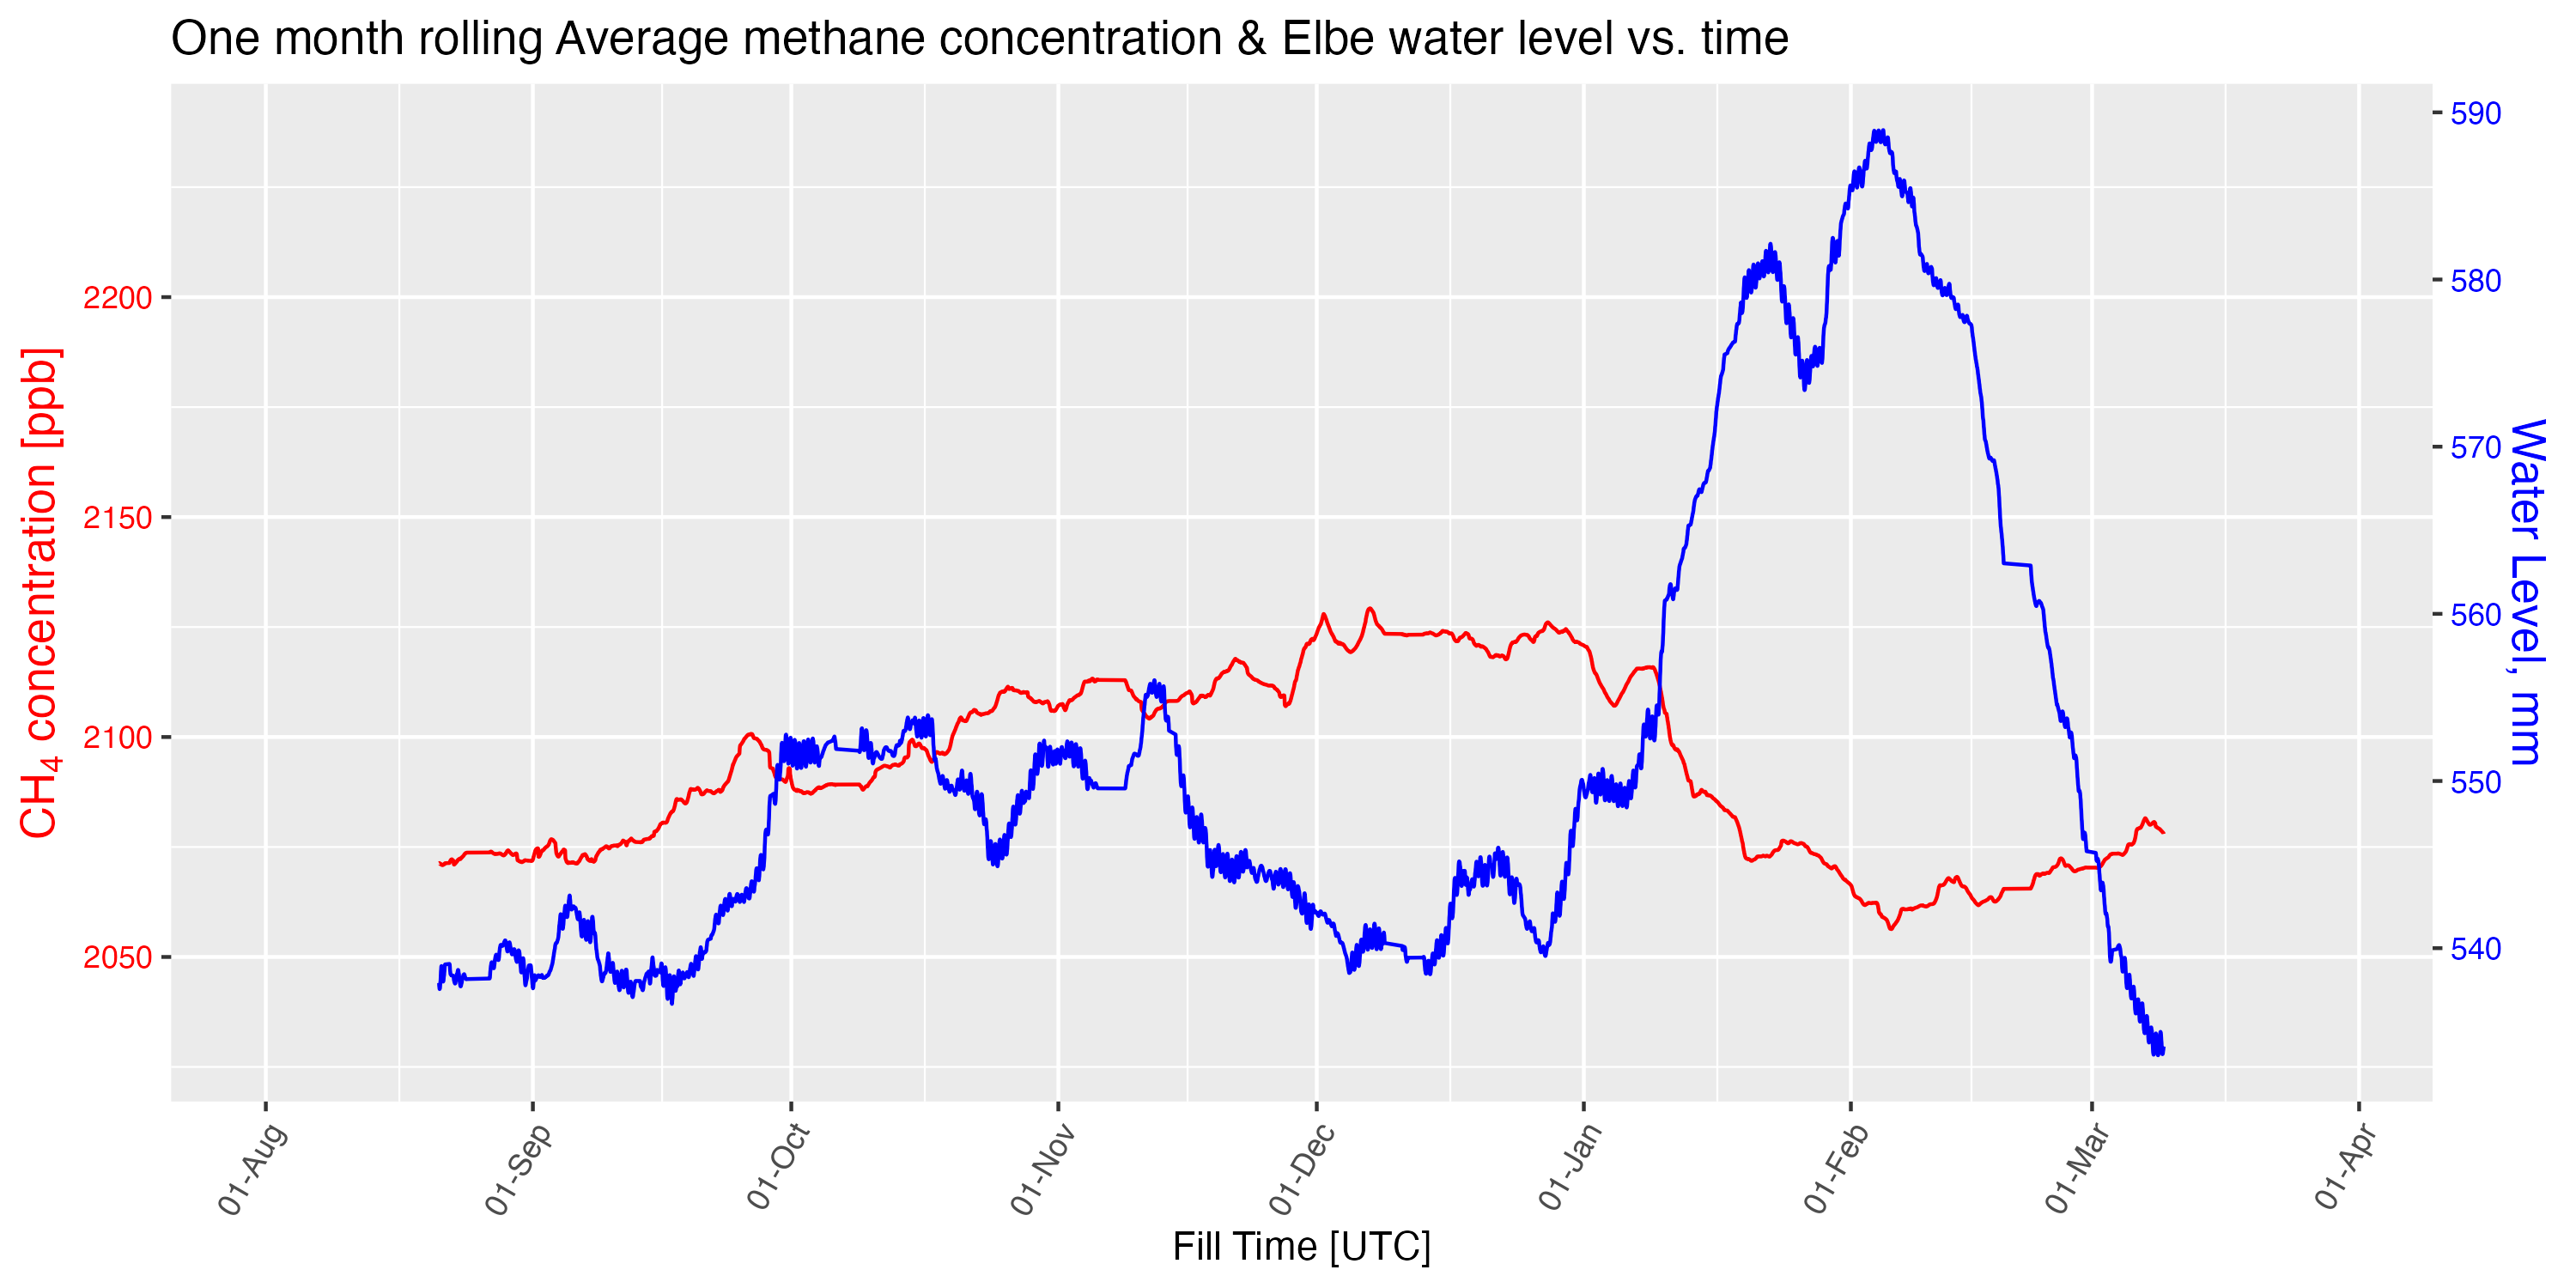
\includegraphics[width=1\textwidth]{figures/Appendix/Water_Level/1_CH4_WLRollingAverage.png}
 \caption[Rolling Average of one month CH$_4$ Timeline with Elbe Water level Overlay]{Rolling average timeline plot of CH$_4$ concentration measured with the CF-IRMS at the Geomatikum (Red) overlayed by the water level timeline of the river Elbe (blue).}
 \label{TimelineCH4WaterlevelRollingAverage}
\end{figure}
While a perfect linear correlation between the water level and the methane concentration was not observed when not regarding  the wind direction and speed. The correlations that were observed, for particular wind directions and speeds, indicate that a significant amount of methane measured at the Geomatikum originates from the Elbe that also correlates to its tidal movements.

\subsection{Elbe water quality methane correlation}
The water quality parameters measured at Elbe Seemannshöft provided by Hamburg Service were used \cite{IHUW.20230501} and were also investigated using Pearson's correlation coefficient and the P-value test. The influence of the Elbe can be seen in a particular region of wind direction and wind speeds in the resulting binned correlation plots \cref{CorrelationWaterQuality}. This region is around 180° to 300° for a wind speed between 1.5 m/s to 7 m/s. And are highlighted by blue circles in the plots. In this general direction from the Geomatikum, the river is located and is most drastically influenced by the tides. Further to the east, a series of locks block the tide in the river, while to the west, the Elbe is significantly wider and more naturalised. \cite{Matousu.2019} has shown a 10 times lower methane concentration in the Elbe in this section.\\
Apart from the water level of the Elbe discussed previously, some water quality parameters also show a good correlation with the methane concentration in the air measured a the Geomatikum.\\
Those include the water temperature, oxygen concentration and saturation, turbidity, UV absorption and pH level. The water temperature is the only parameter that shows a positive correlation this the methane concentration measured at the Geomatikum. All other parameters show a negative correlation with the methane concentration. All previously listed parameters pass the P-value test in the blue highlighted region that represents the general direction of the Elbe.
\begin{figure*}[t!]
    \subfloat[Water Temperature]{%
        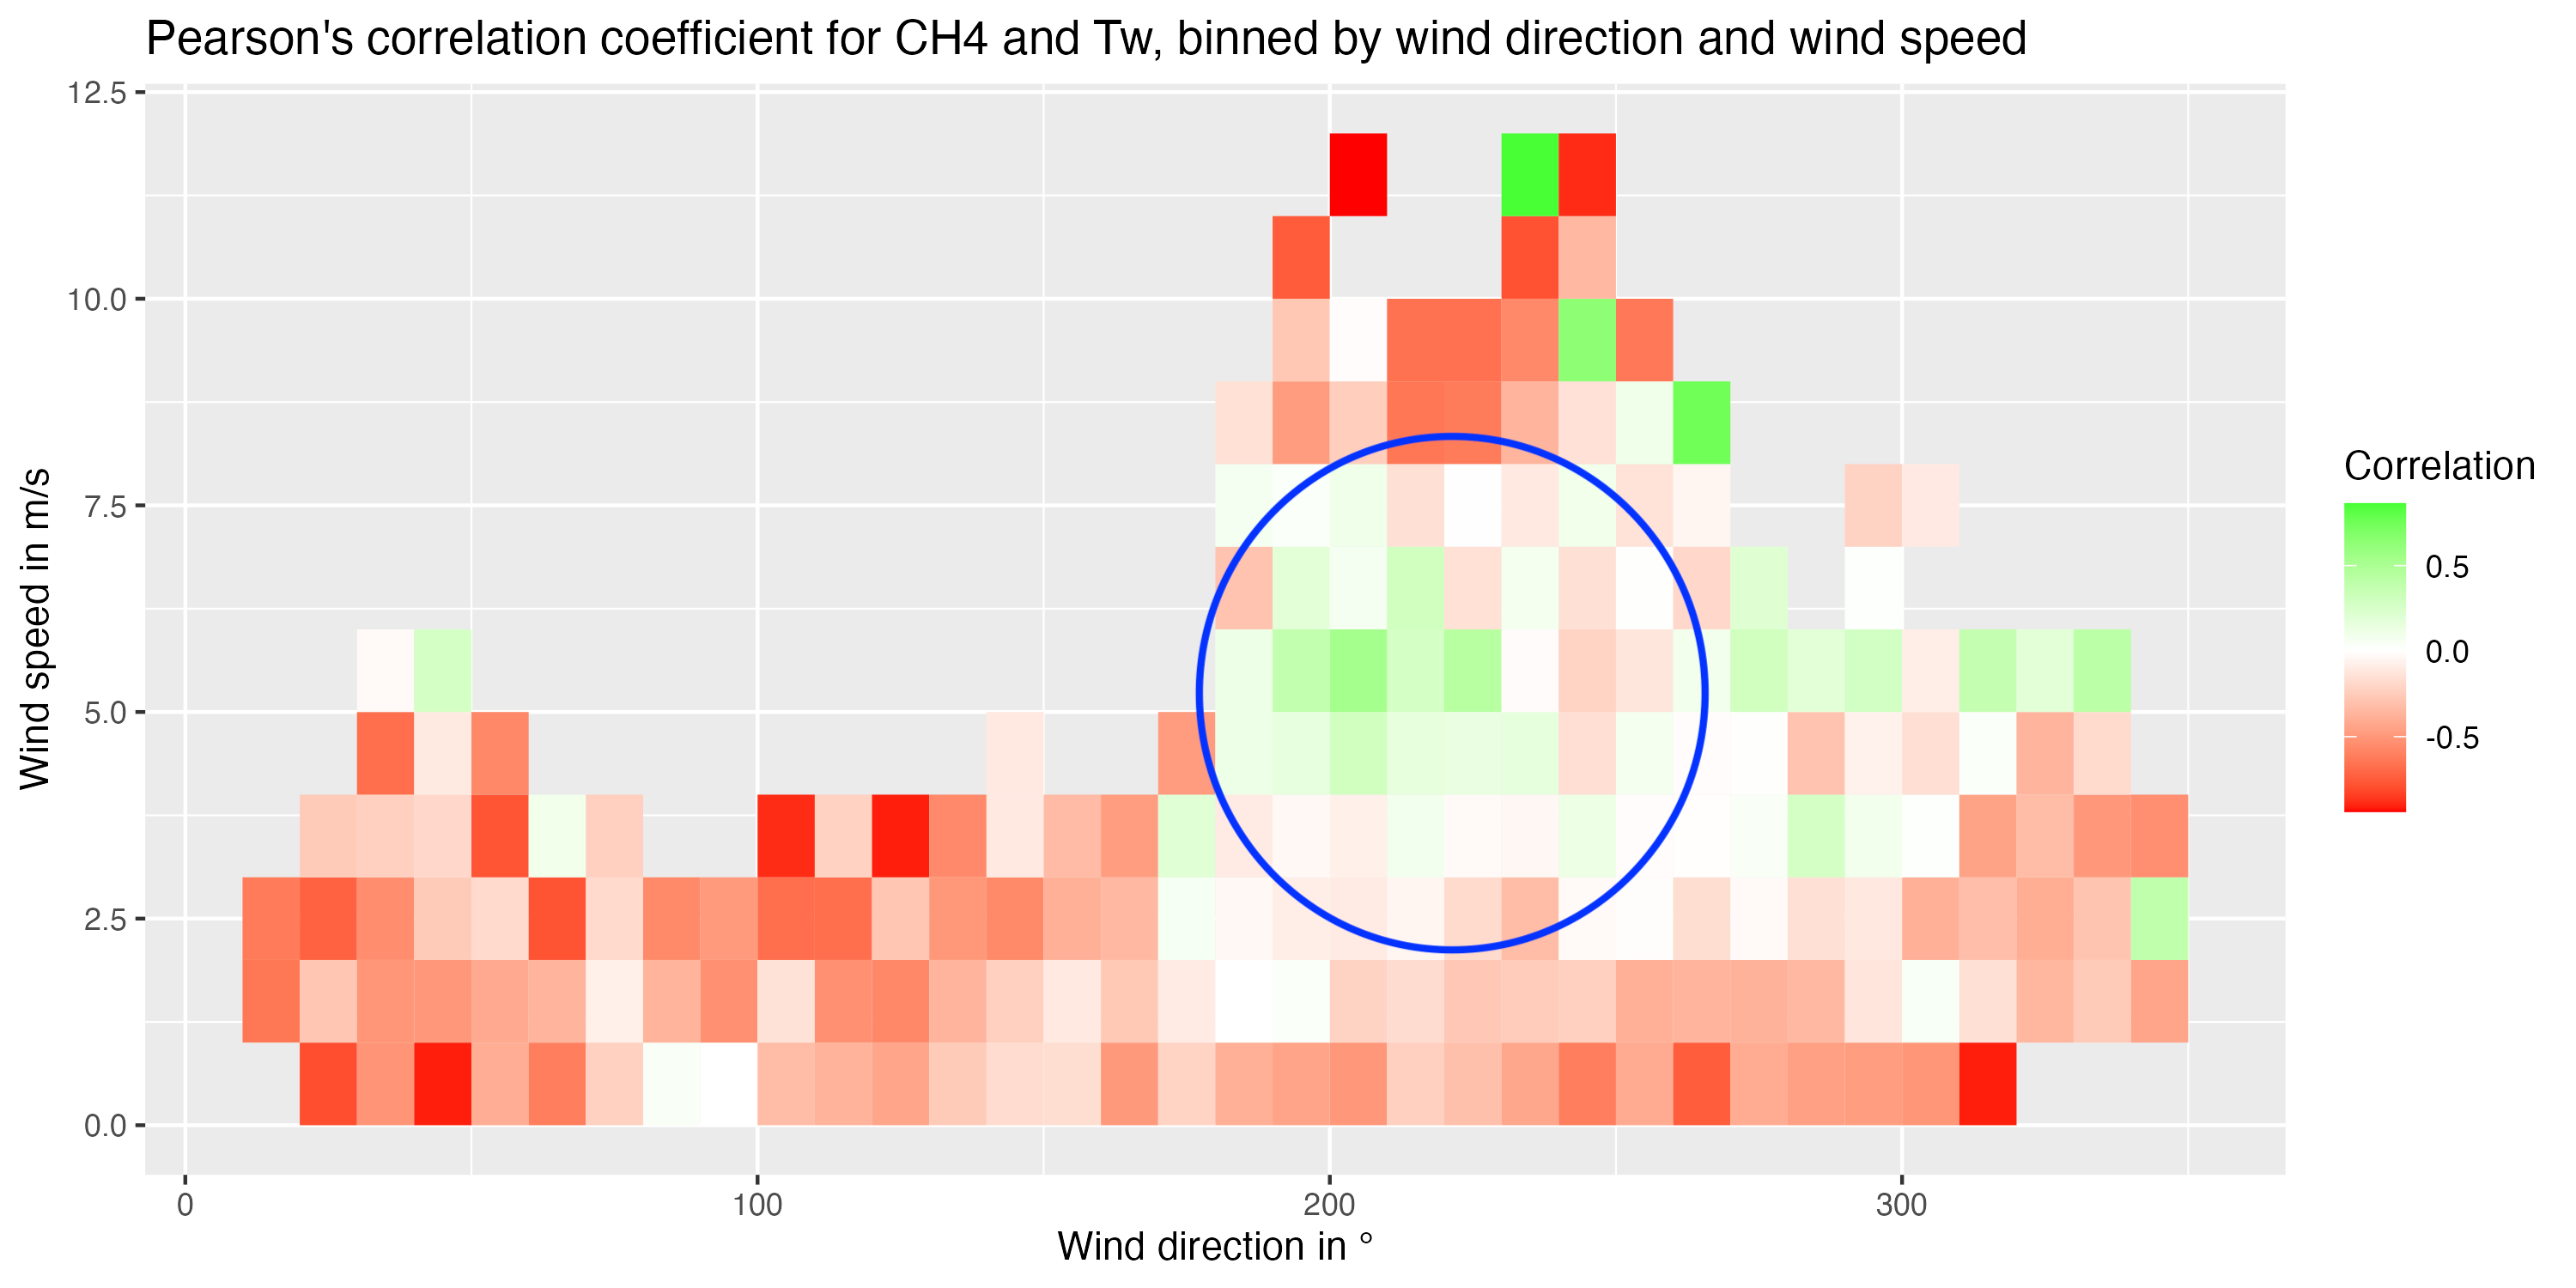
\includegraphics[width=.48\linewidth]{figures/Appendix/Water_Quality/13_CH4_vs_Water_Temp_Correlation_Geomatikum.png}%
        \label{CorrWaterTemp}%
    }\hfill
    \subfloat[O$_2$ concentration]{%
        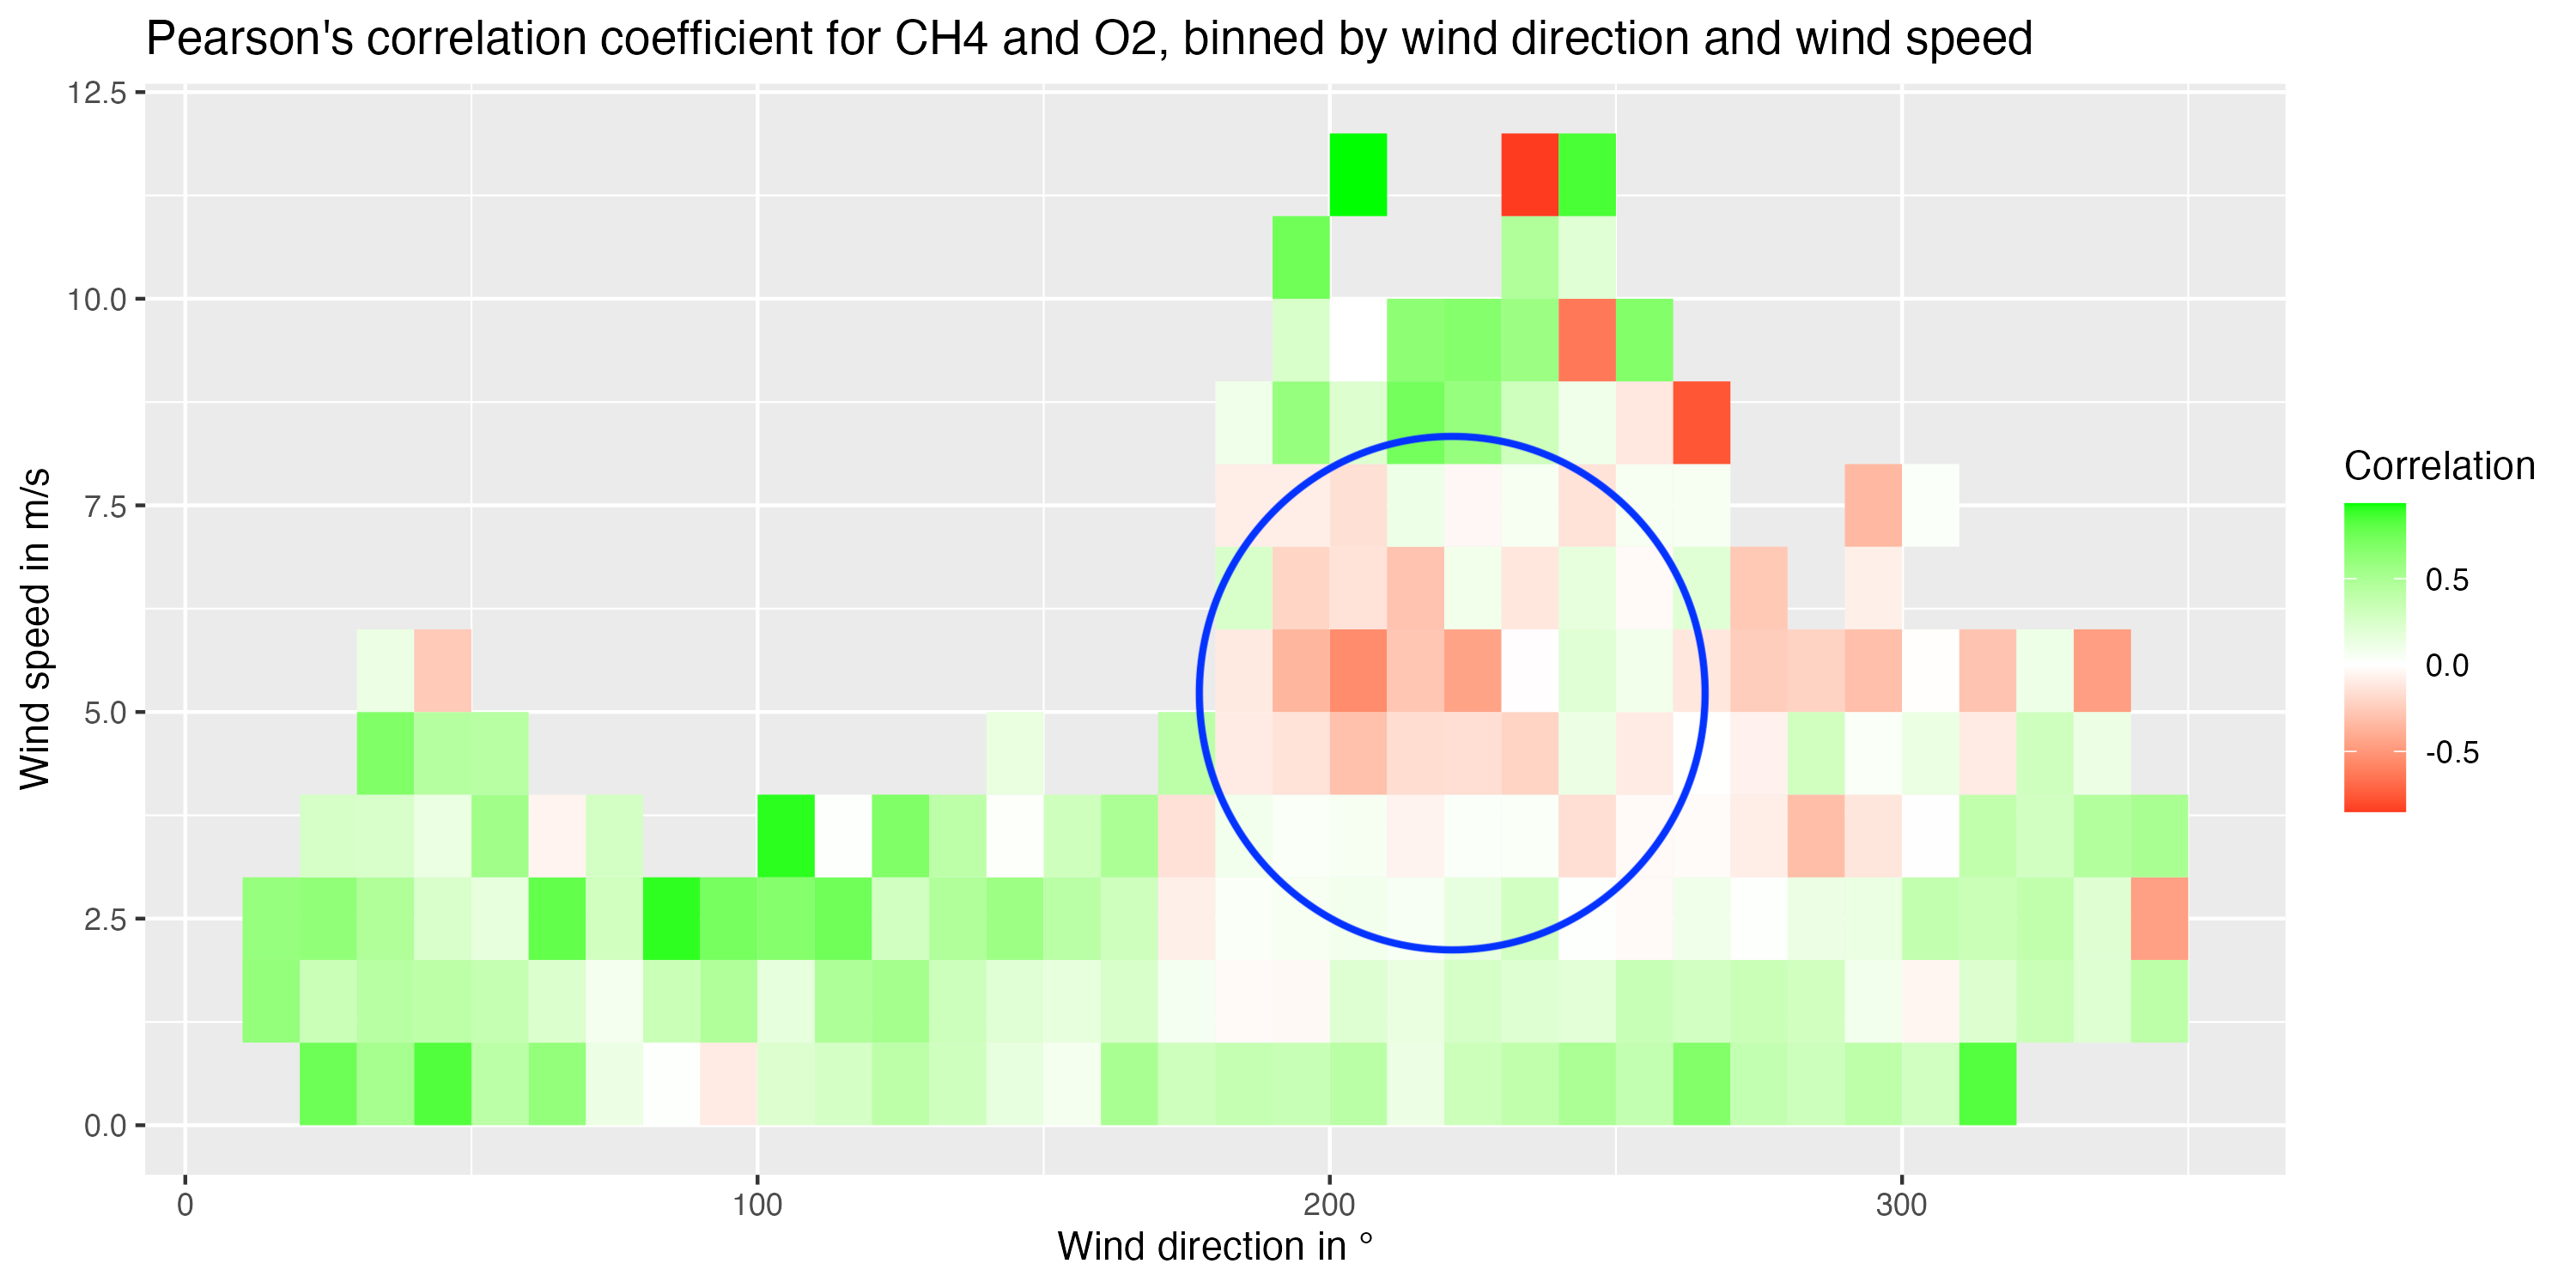
\includegraphics[width=.48\linewidth]{figures/Appendix/Water_Quality/13_CH4_vs_O2_Correlation_Geomatikum.png}%
        \label{CorrO2}%
    }\\
    \subfloat[pH-value]{%
        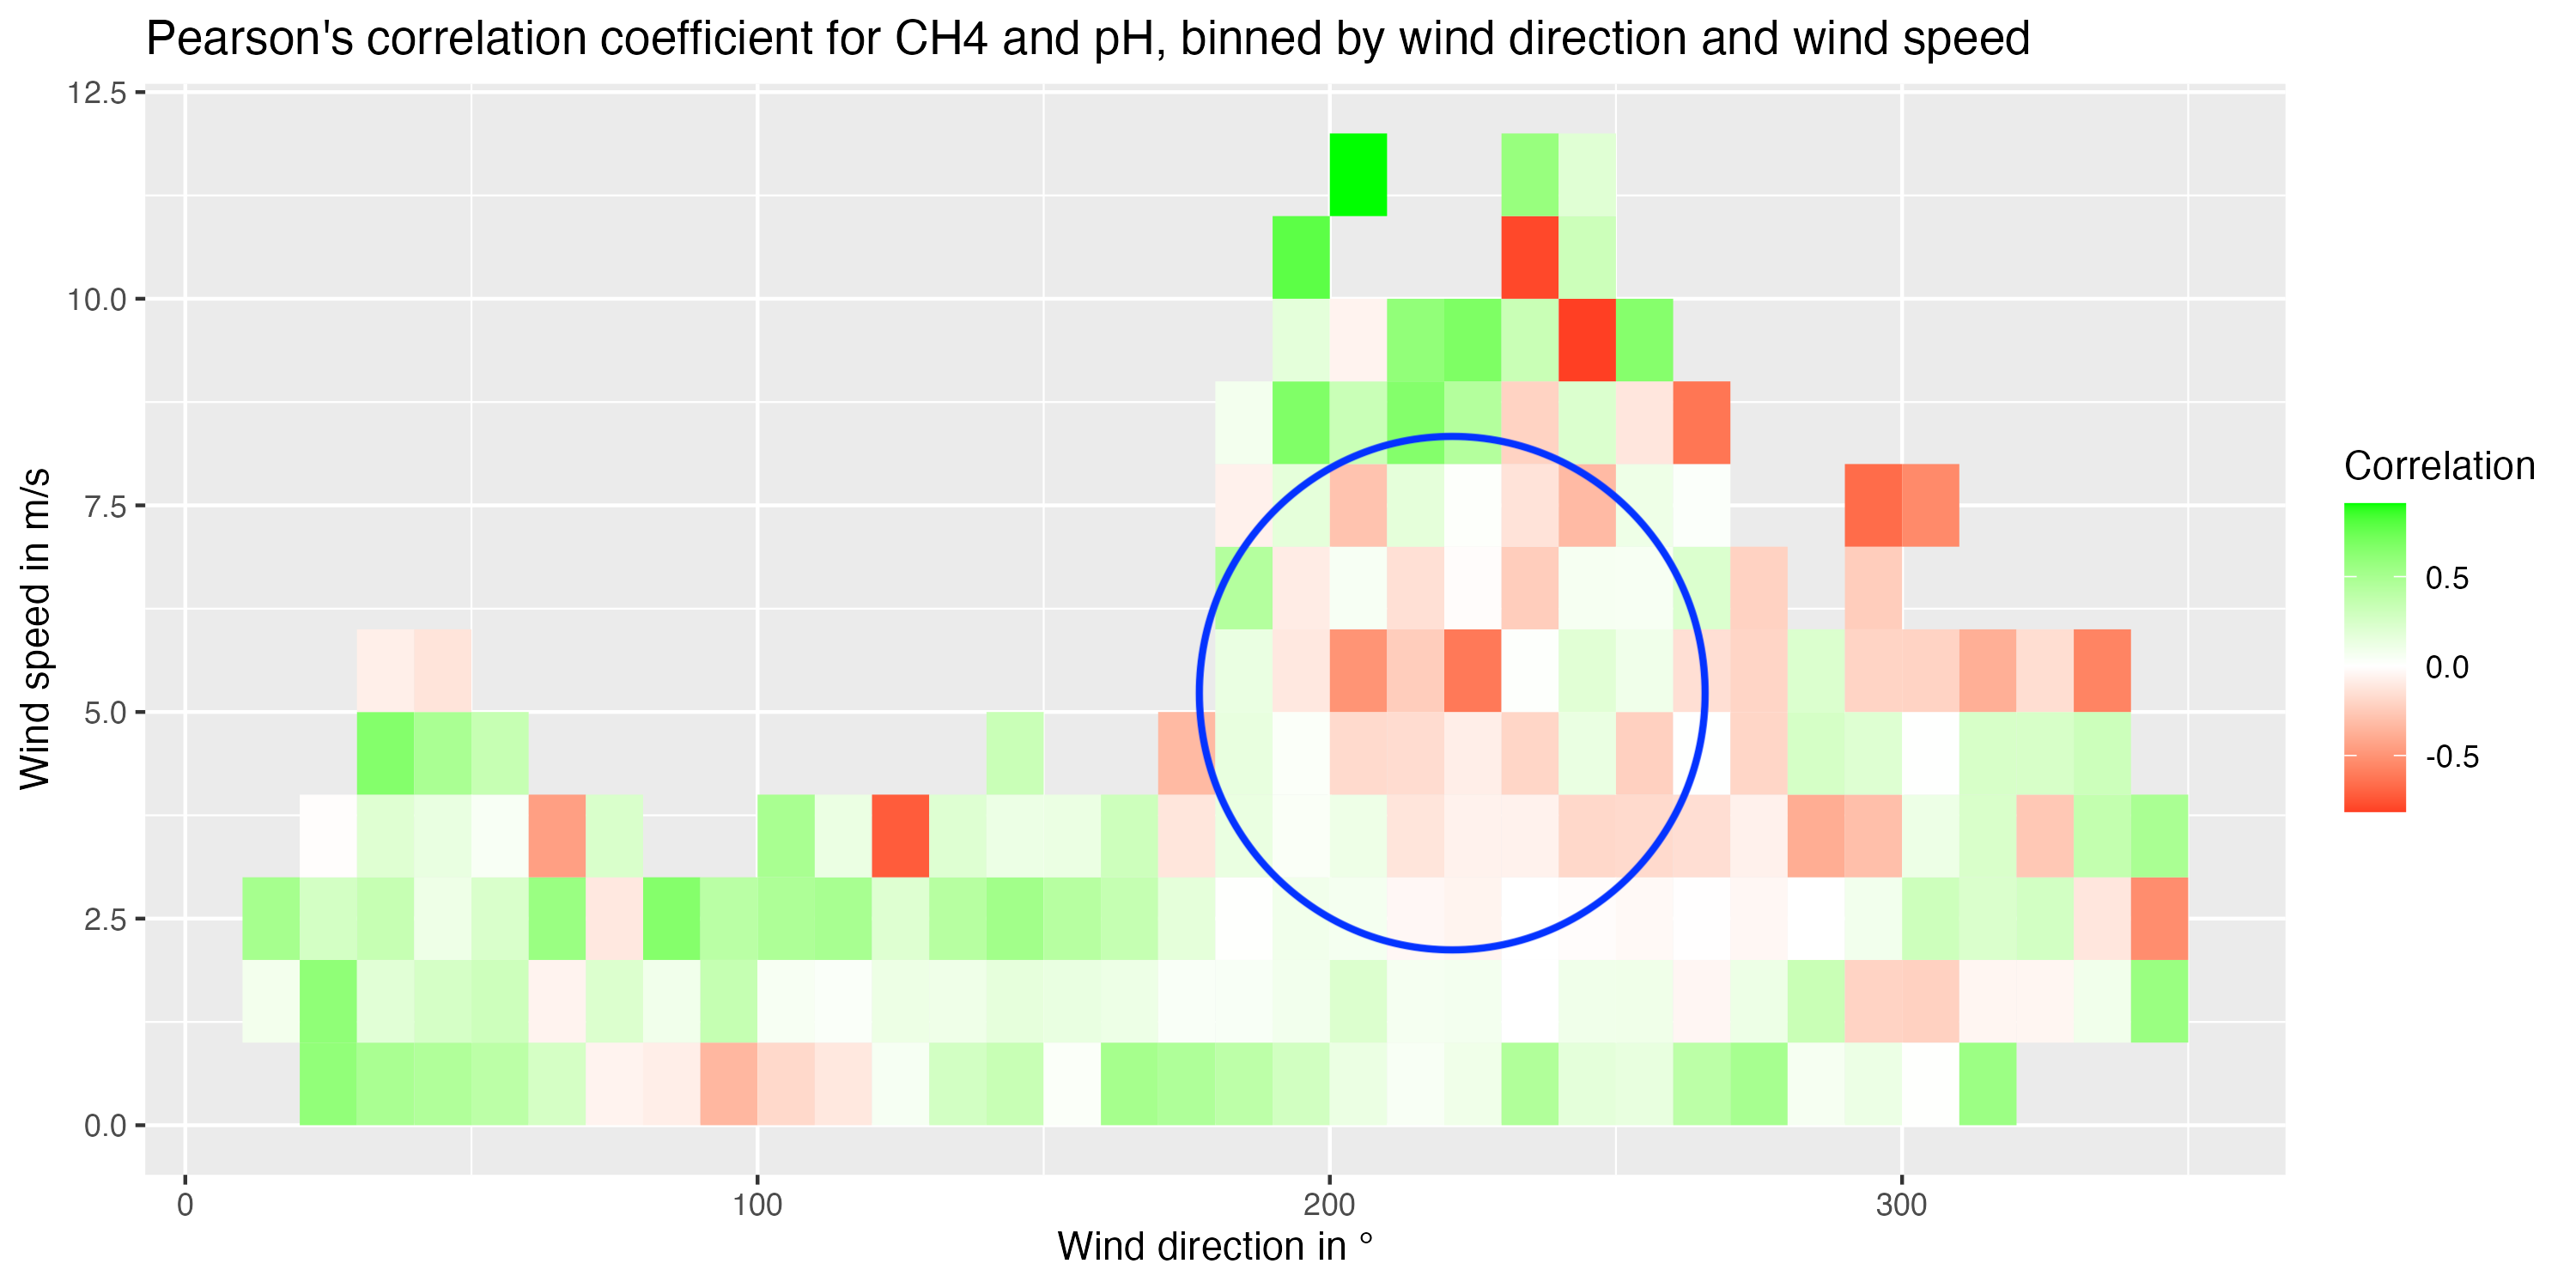
\includegraphics[width=.48\linewidth]{figures/Appendix/Water_Quality/13_CH4_vs_pH_Correlation_Geomatikum.png}%
        \label{CorrPH}%
    }\hfill
    \subfloat[Turbidity]{%
        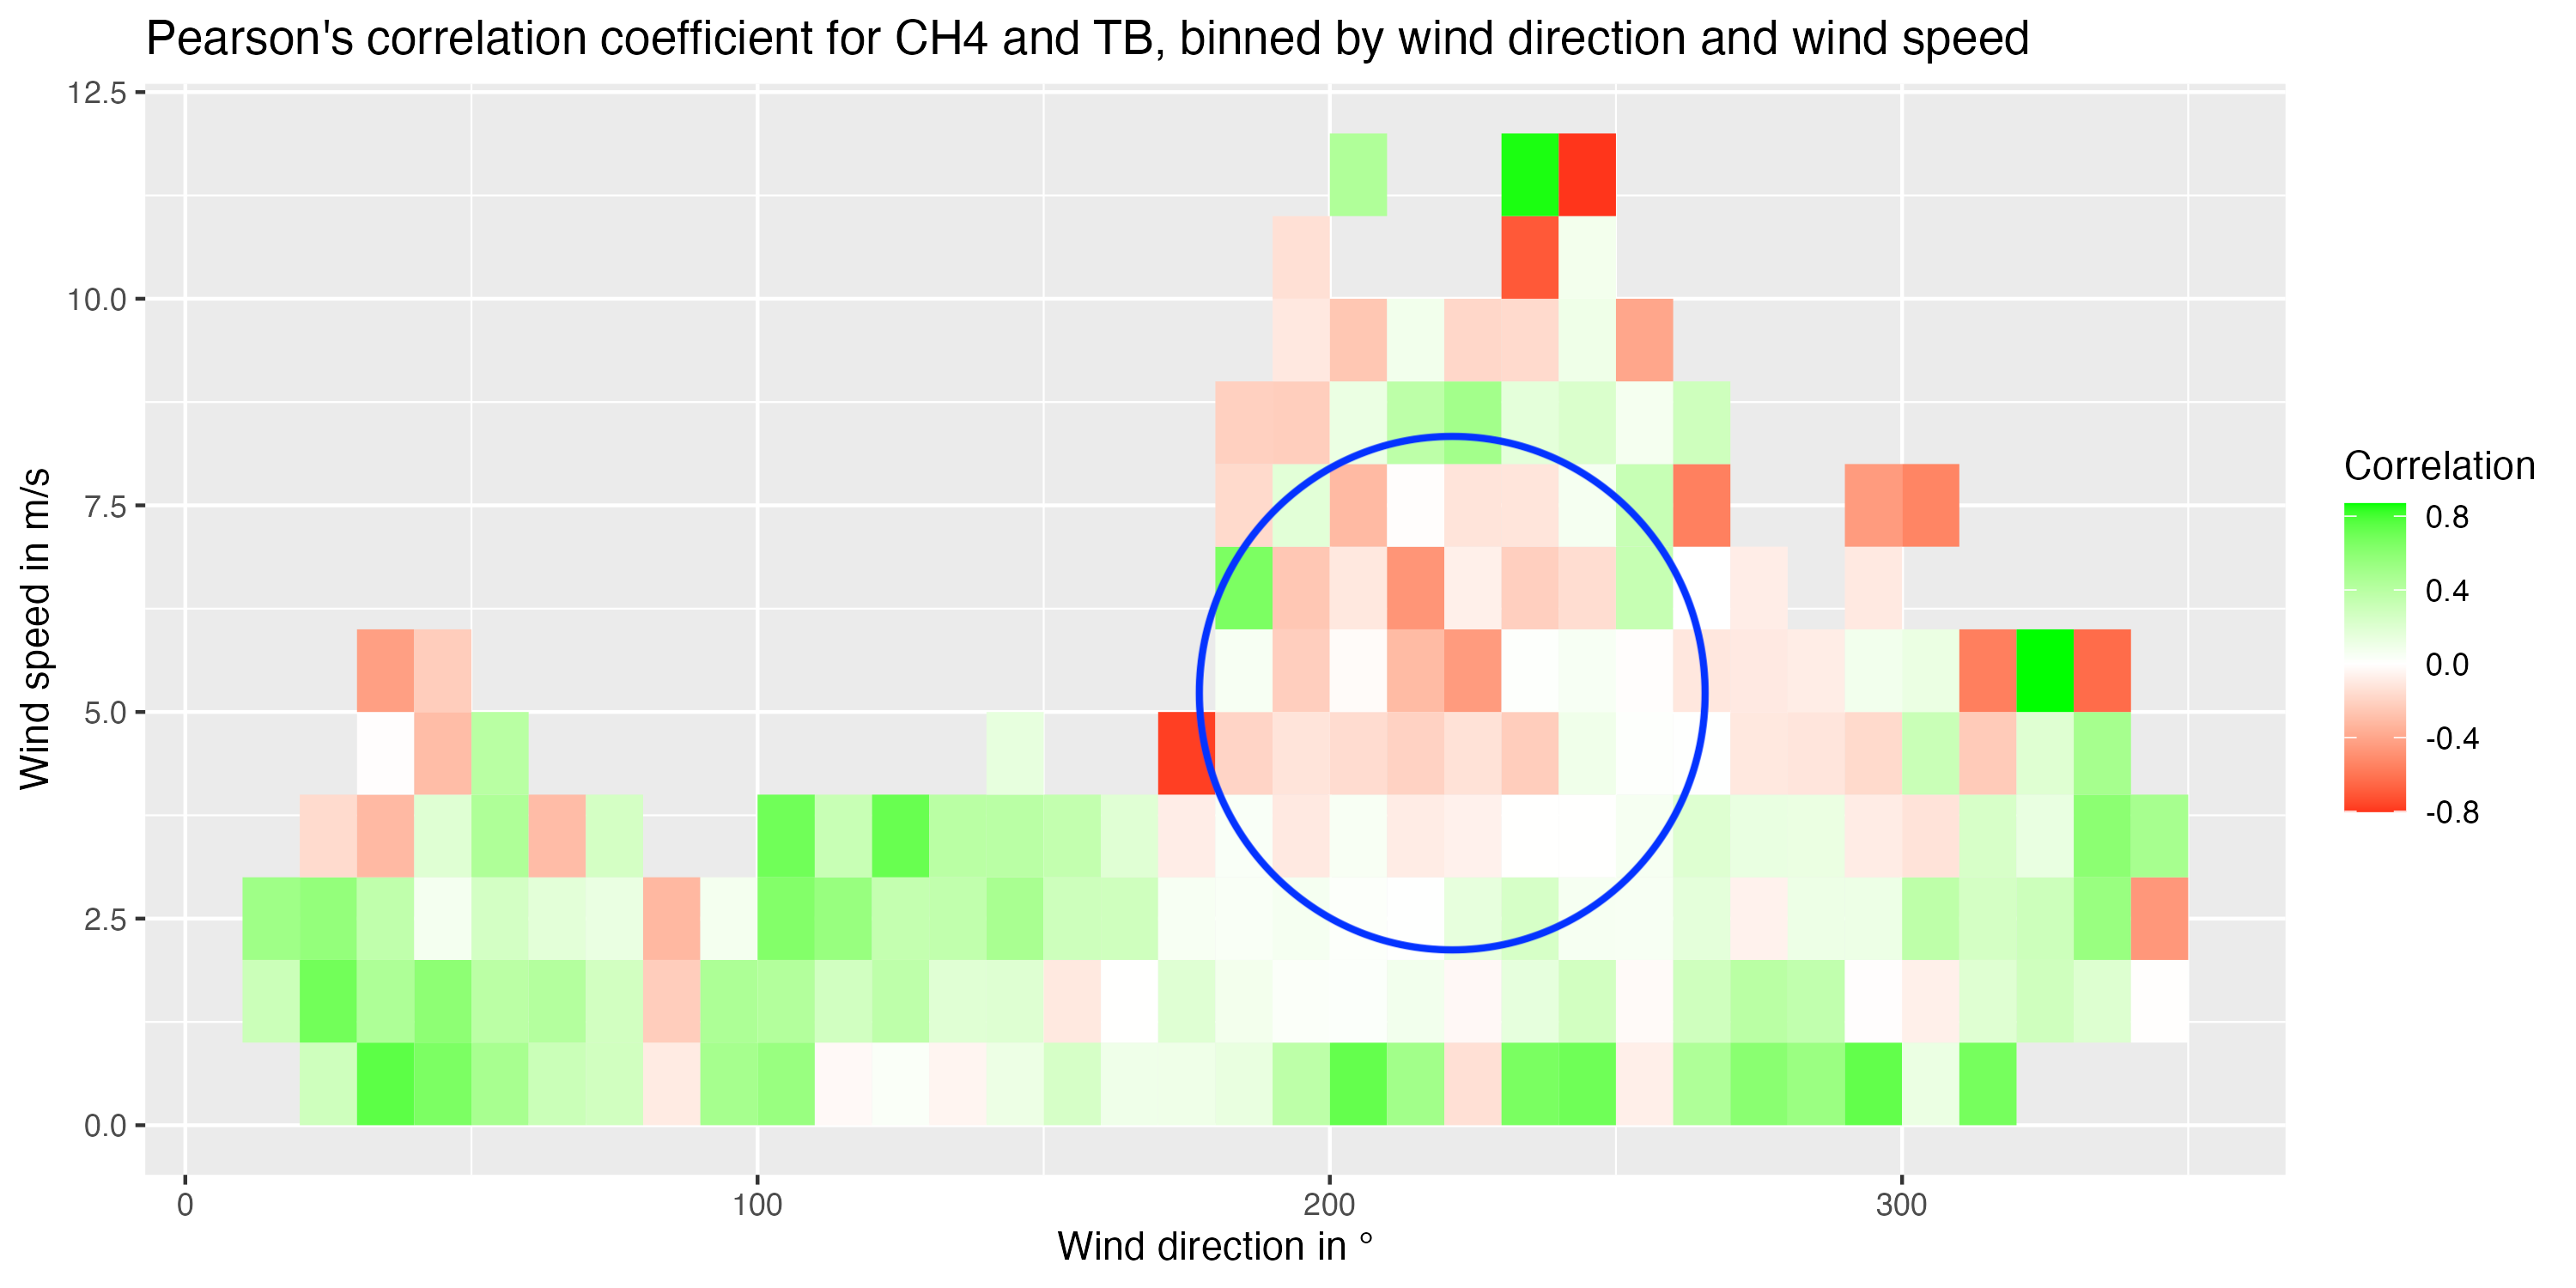
\includegraphics[width=.48\linewidth]{figures/Appendix/Water_Quality/13_CH4_vs_Turbidity_Correlation_Geomatikum.png}%
        \label{CorrTur}%
    }
    \caption[Correlation between CH$_4$ and Water quality]{Pearson's correlation coefficient between methane-air concentration and Elbe water quality parameters, binned by wind direction and wind speed. Green shows a positive correlation (enhanced CH$_4$ at high values), and Red shows a negative correlation (enhanced CH$_4$ at values). The blue circles indicate the wind direction and speed where the Elbe has a strong influence.}
    \label{CorrelationWaterQuality}
\end{figure*}
Other water quality parameters, such as electrical conductivity and algae concentrations (Chlorophyll concentration of various different species), don't show a correlation with the measured methane concentration. Those parameters don't seem to influence the microbial health in the Elbe significantly enough to influence their methane production and reduction mechanisms substantially.

\subsection{Meteorological observation and methane correlation}
%needs correction!!!!
The meteorological data measured by the DWD at Hamburg-Fuhlsbüttel \cite{DeutschenWetterdienst.20230501} was investigated in the same manner as the water parameters of the Elbe.
Pearson's correlation coefficient and P-value test for the meteorological parameter with the methane concentration in the air show some correlations between them. Those include air temperature, solar radiation, dewpoint and humidity.\\
The humidity and dewpoint measurements have a general correlation for all wind directions and speeds, excluding the region 180° - 300° and (0.5 to 3.5 m/s). In this region, no significant correlation can be observed. This can be seen in \cref{CorrHumid} and \cref{CorrDewPoint}, where the black circle indicates this region. Following these wind directions and considering the low wind speeds leads to the densely urbanised city centred, where very few natural areas such as parks and gardens are present.\\
The temperature and solar radiation correlate significantly with the methane concentration. A negative correlation is observed in nearly all regions, only excluding the 180° - 250° and (1.5 to 7 m/s) region. In this wind direction, the Elbe is located, and the methane emissions from the Elbe seem to dominate in this region. In figure \cref{CorrAirTemp} and \cref{CorrRadiation}, this region is indicated by blue circles.
The remaining region shows a significant negative correlation between the temperature and solar radiation with the methane concentration in the air. In particular, the wind directions from 330° to 130° show a very strong negative correlation at all wind speeds. The wind direction in this region point to the primarily residential regions of Hamburg. The Elbe is not present in this region, and no tidal-influenced waterbodies exist there. The Keeling plot analyses with regards to wind direction, which will be discussed later, indicated a strong anthropogenic methane production influence, such as fossil fuel combustion. This is also confirmed by \cite{Maazallahi.2020}, who found numerous gas infrastructure leakages and a generally high anthropogenic methane mixture in this region using street-level mobile measurements. 
\begin{figure*}[t!]
    \subfloat[Humidity]{%
        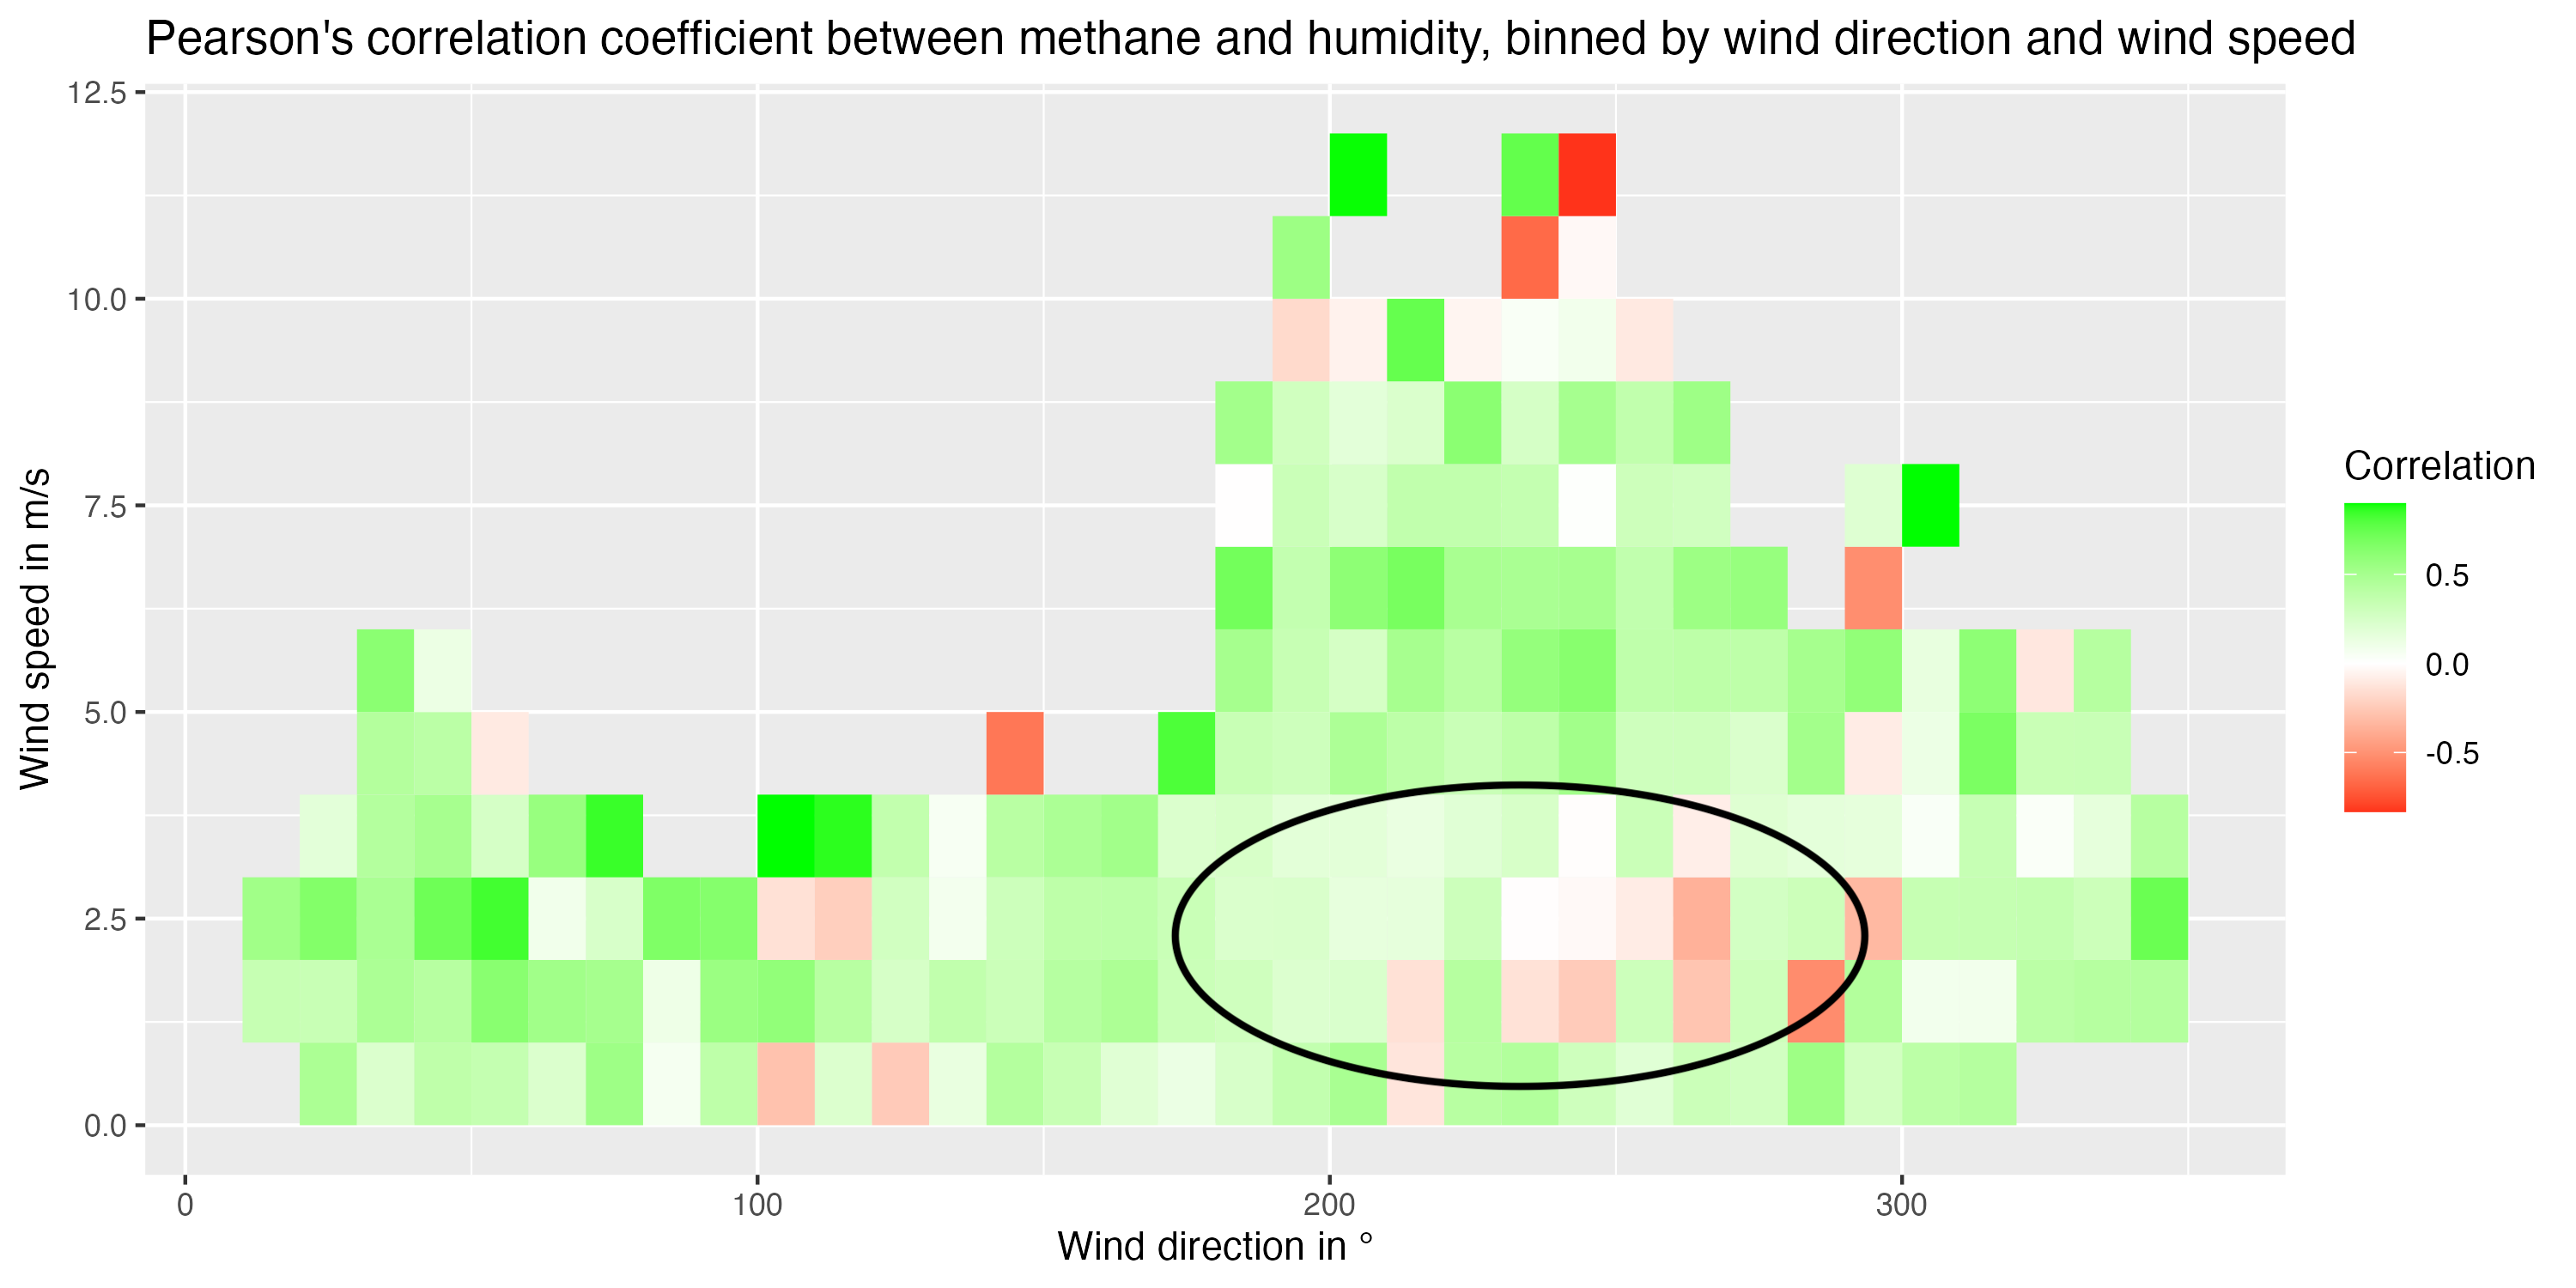
\includegraphics[width=.48\linewidth]{figures/Appendix/Meteorological/13_CH4_vs_humidity_Correlation_Geomatikum.png}%
        \label{CorrHumid}%
    }\hfill
    \subfloat[Dew point]{%
        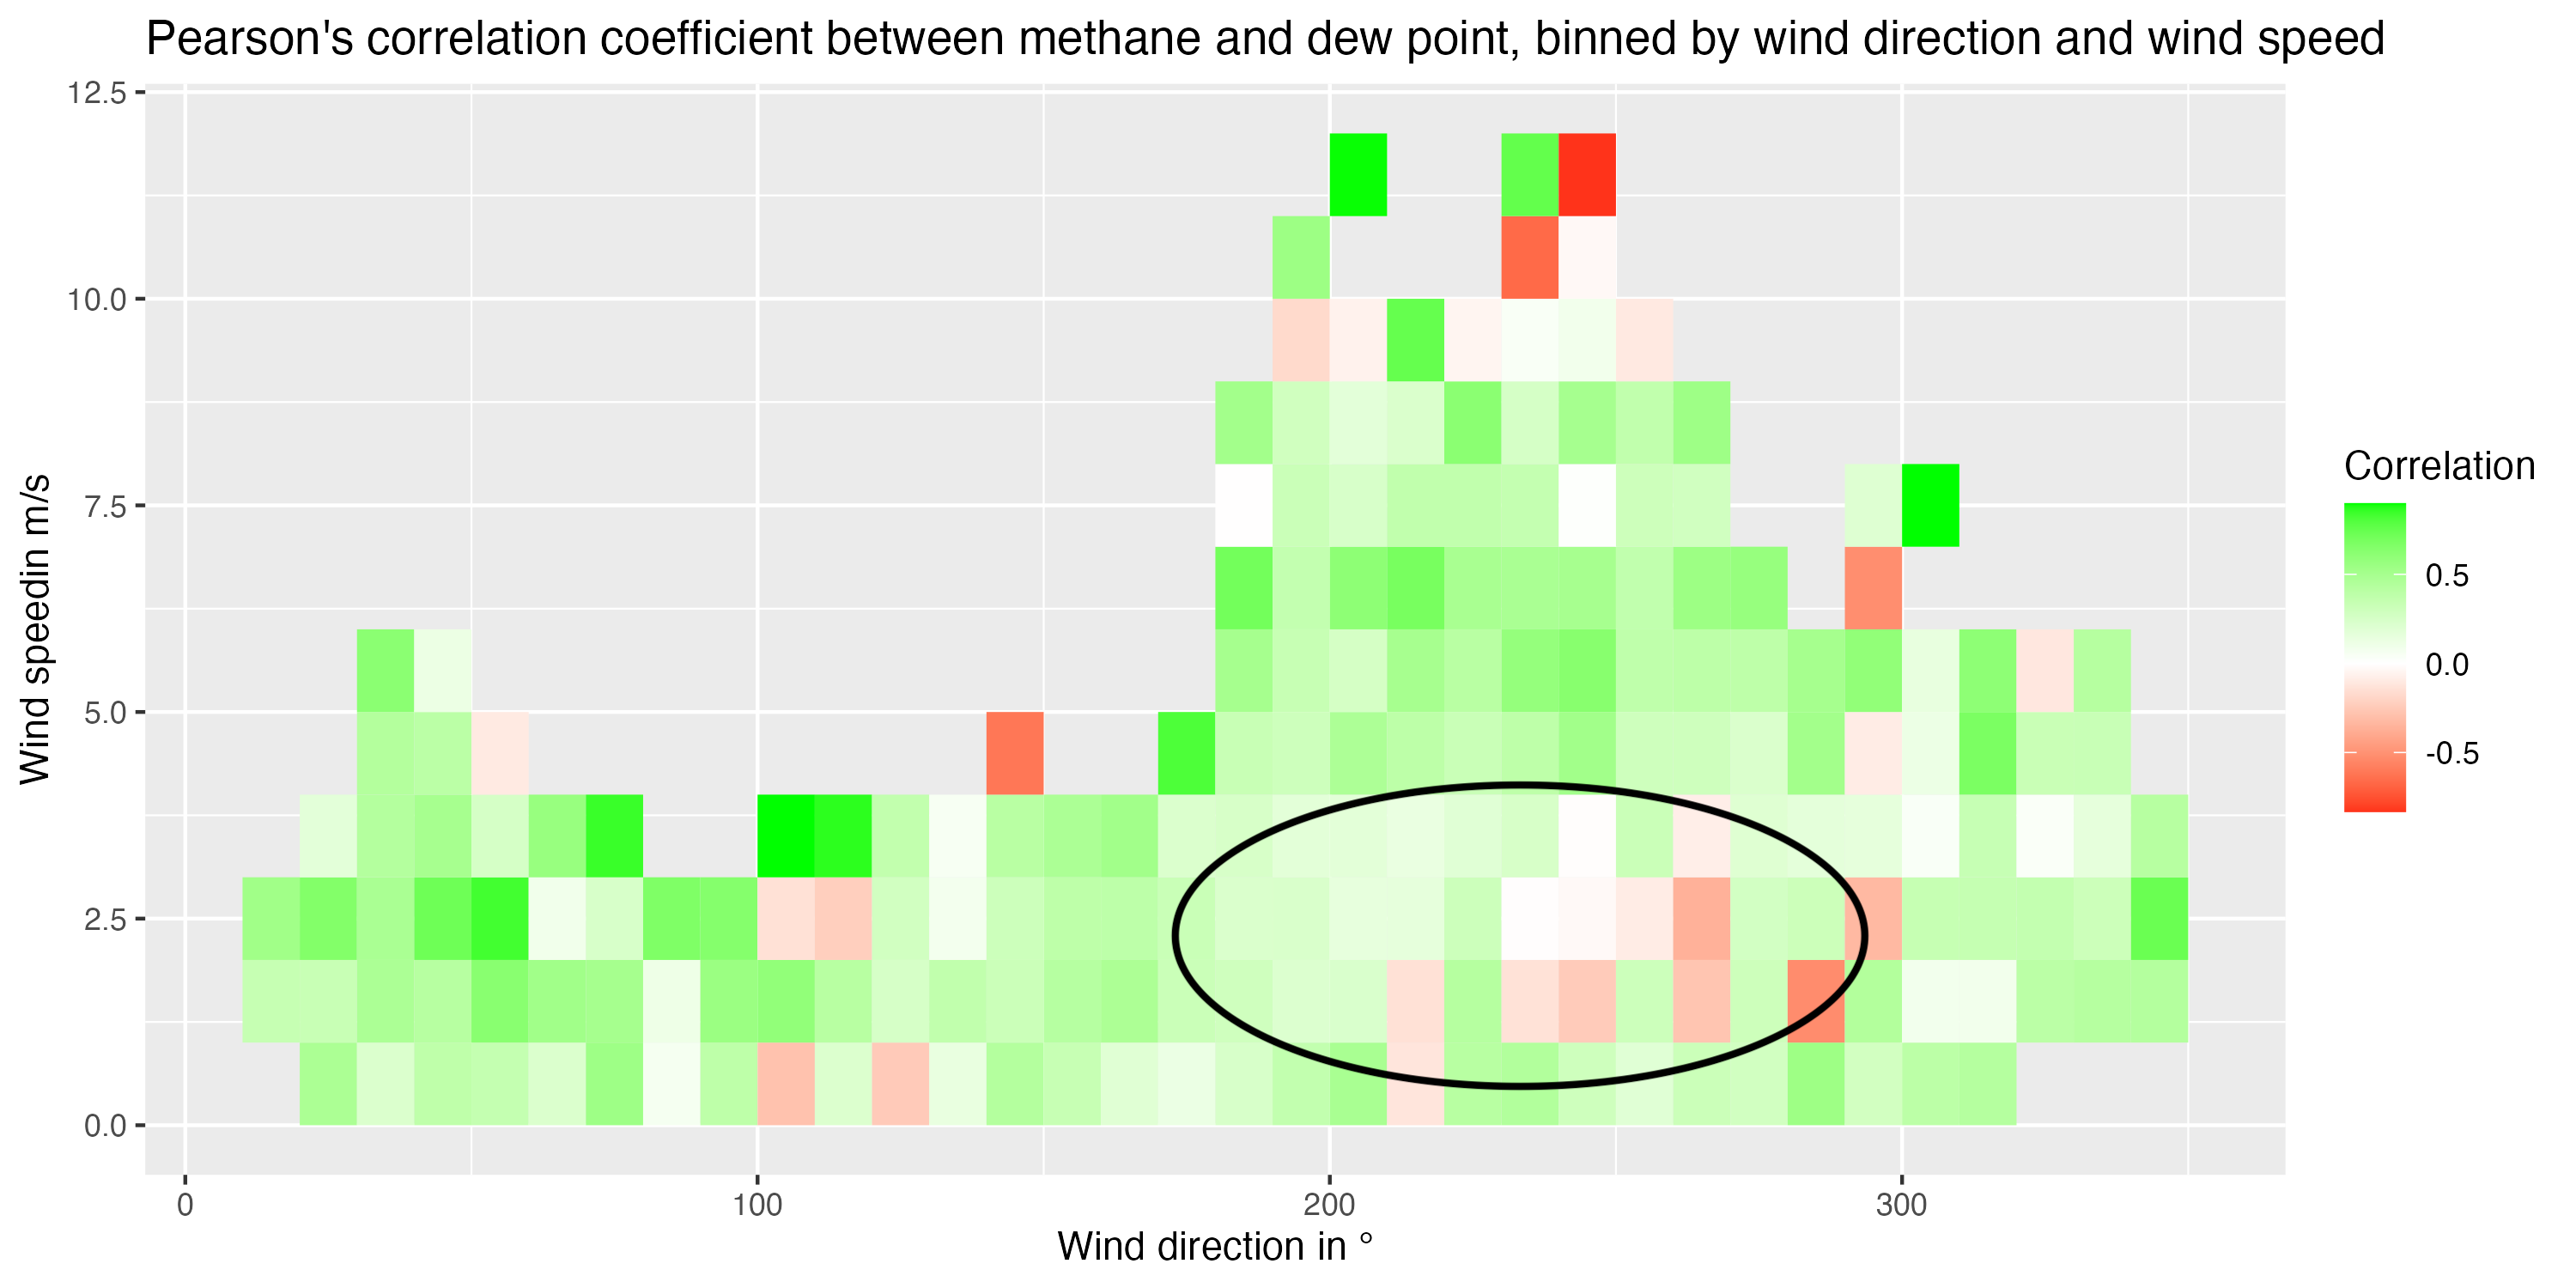
\includegraphics[width=.48\linewidth]{figures/Appendix/Meteorological/13_CH4_vs_dew_point_Correlation_Geomatikum.png}%
        \label{CorrDewPoint}%
    }\\
    \subfloat[Air temperature]{%
        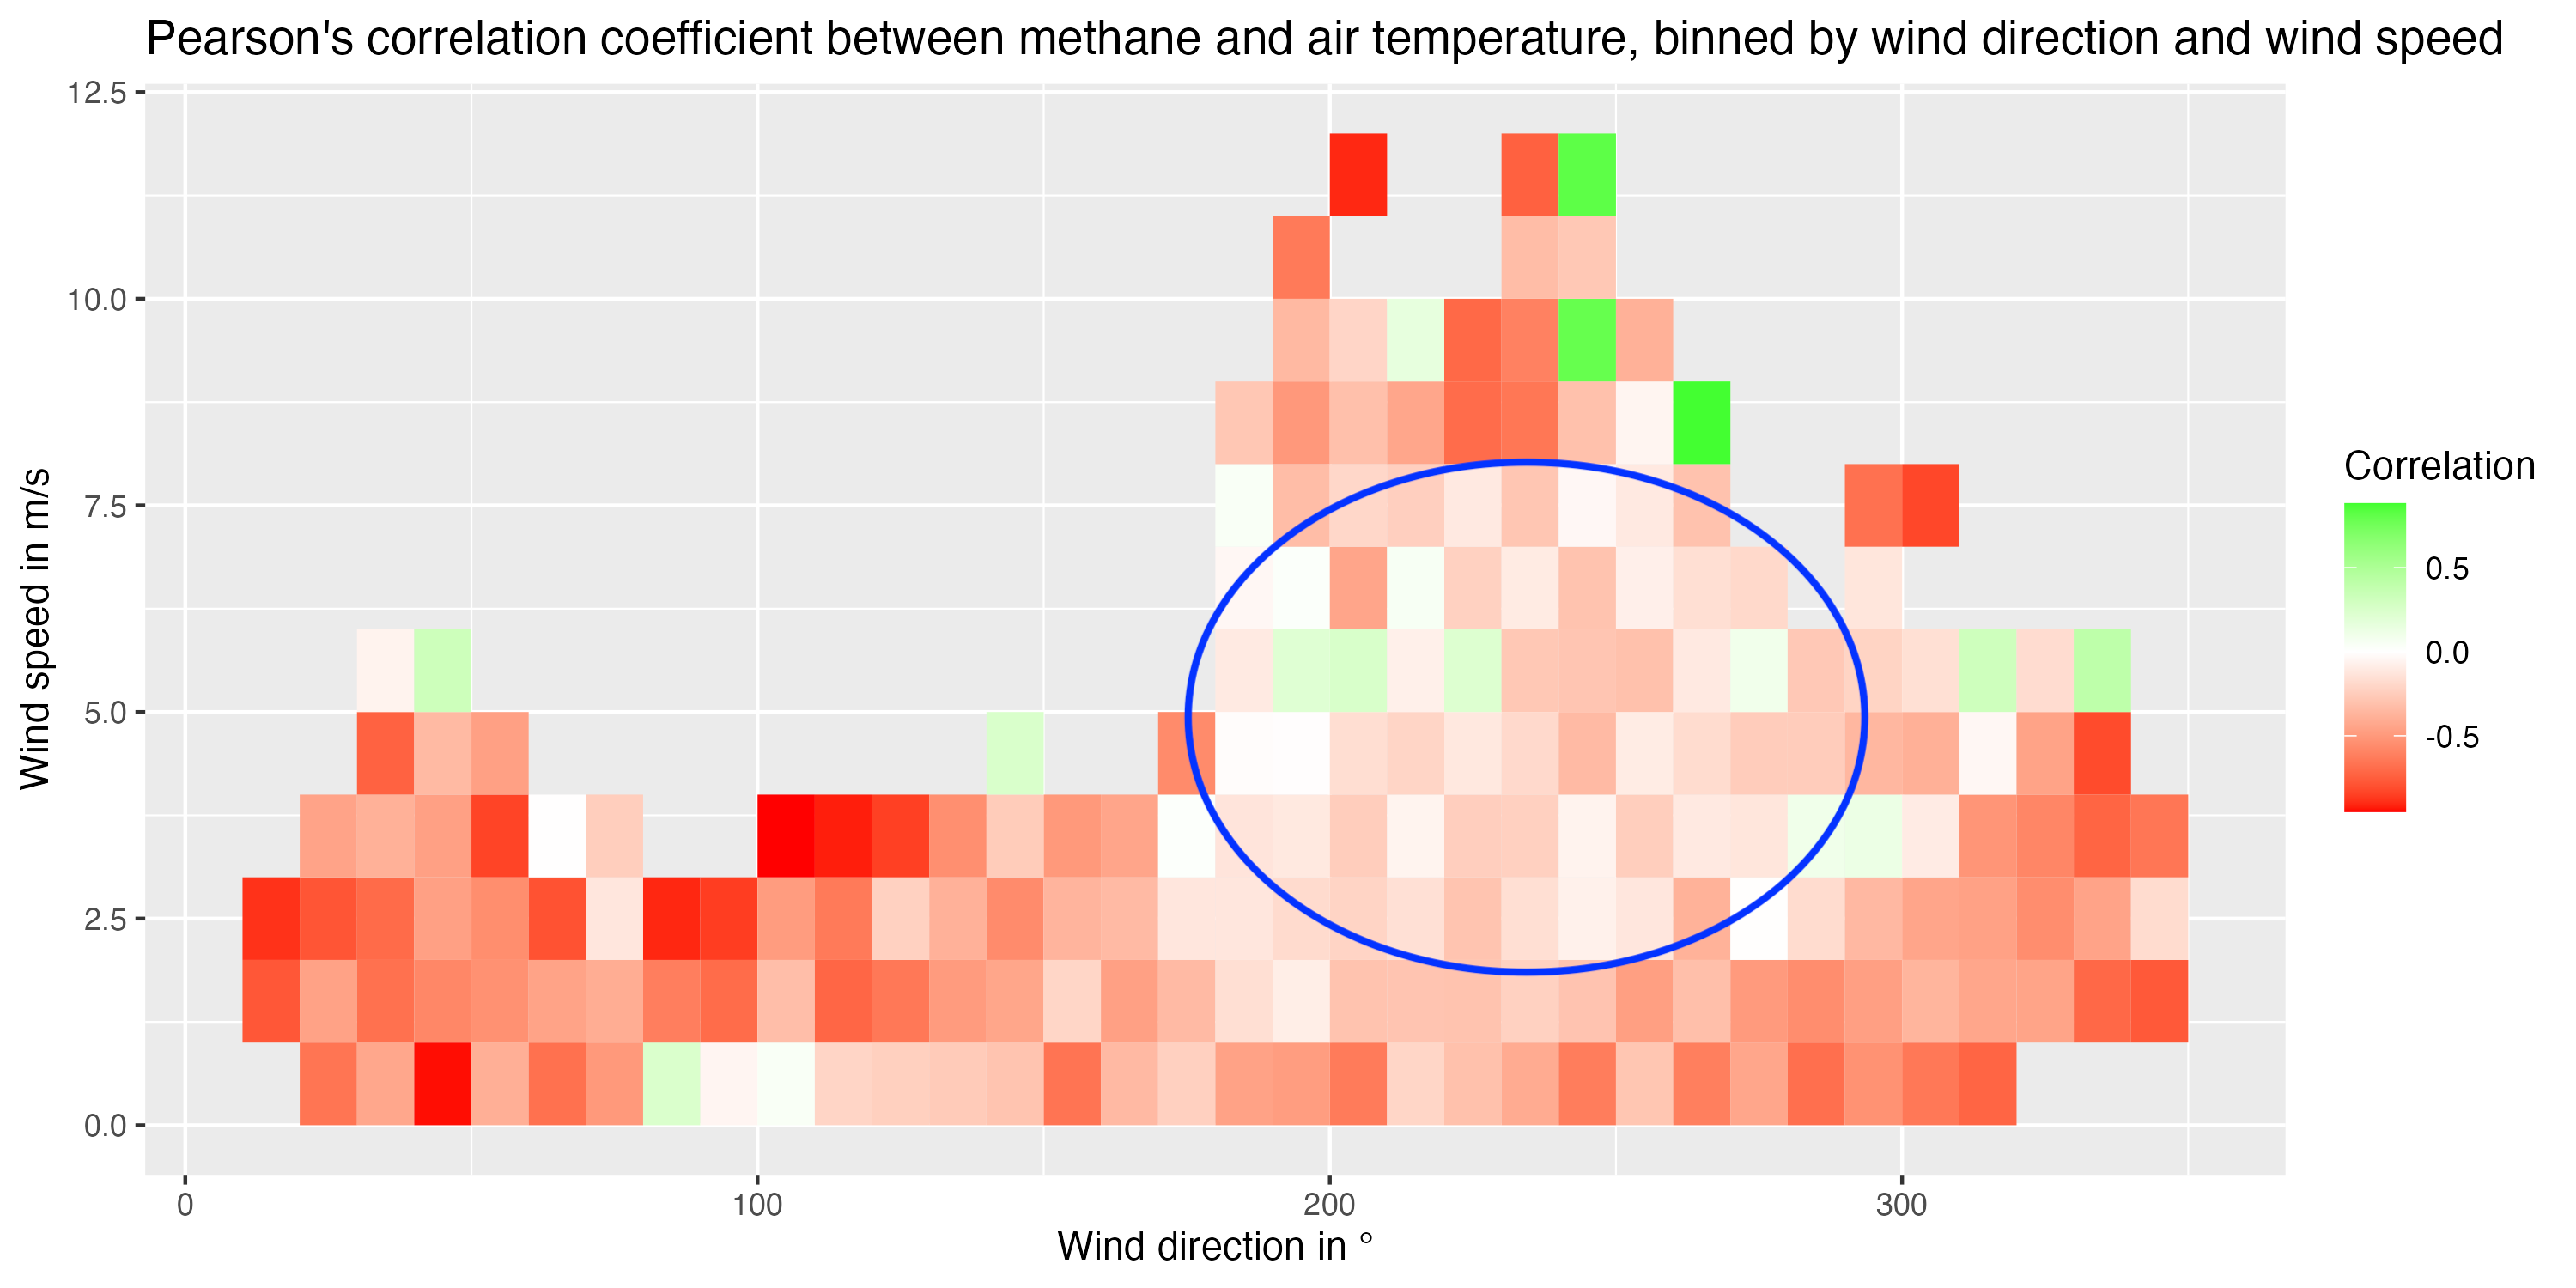
\includegraphics[width=.48\linewidth]{figures/Appendix/Meteorological/13_CH4_vs_temperature_Correlation_Geomatikum.png}%
        \label{CorrAirTemp}%
    }\hfill
    \subfloat[Radiation]{%
        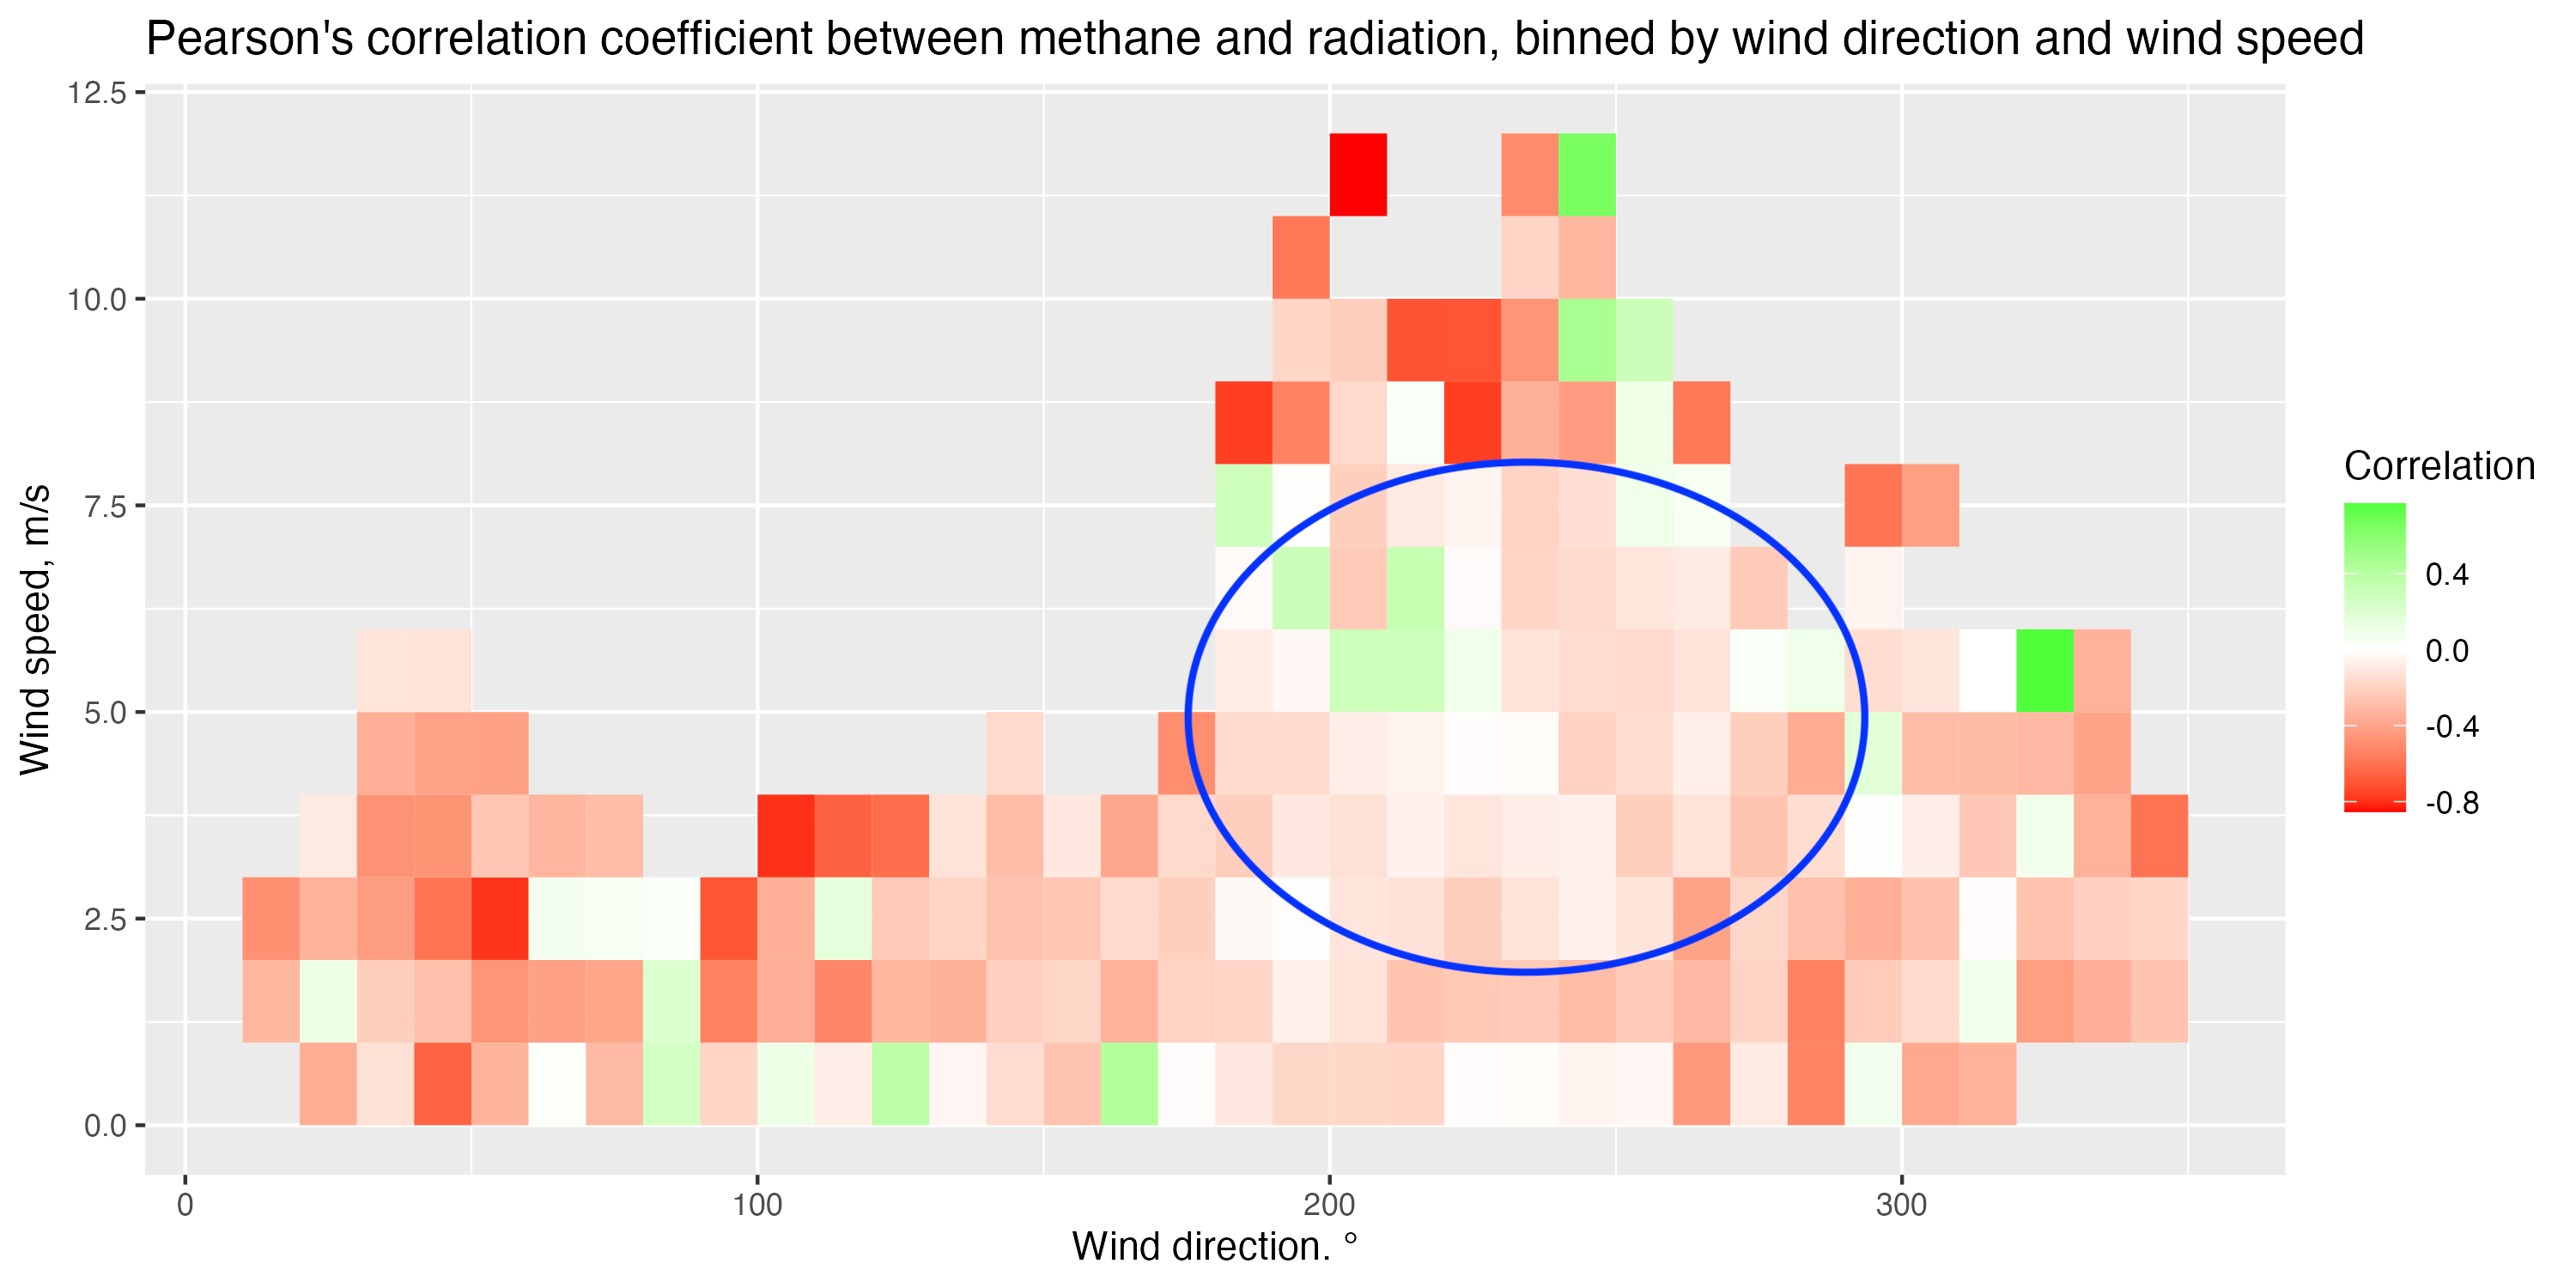
\includegraphics[width=.48\linewidth]{figures/Appendix/Meteorological/13_CH4_vs_radiation_Correlation_Geomatikum.png}%
        \label{CorrRadiation}%
    }
    \caption[Correlation between CH$_4$ and meteorological data]{Pearson's correlation coefficient between methane-air concentration and Meteorological data, binned by wind direction and wind speed. Green shows a positive correlation (enhanced CH$_4$ at high values), and Red shows a negative correlation (enhanced CH$_4$ at low values). The black circles indicate a region with no correlation, potentially the city centre of Hamburg. The blue circles indicate the region where the Elbe is located.}
    \label{CorrelationMeteorological}
\end{figure*}
Other meteorological parameters were investigated, such as precipitation and air pressure, etc. For those parameters, no correlation with the methane concentration in the air measured at the Geomatikum could be observed.

\subsection{Wind analysis and methane correlation}
By analysing and implementing the wind measurements provided form the DWD and Hamburg Universiät, the data measured at the Geomatikum proved to yield the most reliable results. The measurements by the DWD at Hamburg-Fuhlsbüttel suffered from its low measurement altitude consequent high variability due to disturbances by the topography, \cref{WindRoseAppendix}. The measurements at the weather mast in Hamburg Billbrook showed good turbulent-free results. But due to the large distance between the CF-IRMS measurement location and the weather mast of 17 km the measurements showed a temporal mismatch between the two measurement series. The measurements at the Geomatikum proved the most reliable due to proximity to the CF-IRMS measurement and the relatively low disturbance due to the measurement height of 83m. In the modelling, discussed later on, the measurements at the Geomatikum also showed the best results.\\
The total measurement series from 01.08.21 to 01.4.2022 showed that dominant wind direction could be observed from the South-West with generally medium wind speeds. The Windrose Plot \cref{RoseTotalGeomatikum} show this average wind direction from South-West rather well. While wind from all directions has generally been observed, four distinct patterns were observed, indicating some reoccurring and distinguished weather patterns in Hamburg. Most likely, the westerly winds, high-pressure regions over the mainland and transitions of cyclones into central Europe. By additionally using the methane measurements in a pollution rose plot, one can see that the methane emission does come from every direction with a distribution closely reassembling the wind direction distribution. This shows us that the background methane concentration has no clear emission direction. While the highest concentrations are generally observed more often in South-Western wind directions.
\begin{figure}
\centering
\begin{subfigure}{.5\textwidth}
  \centering
  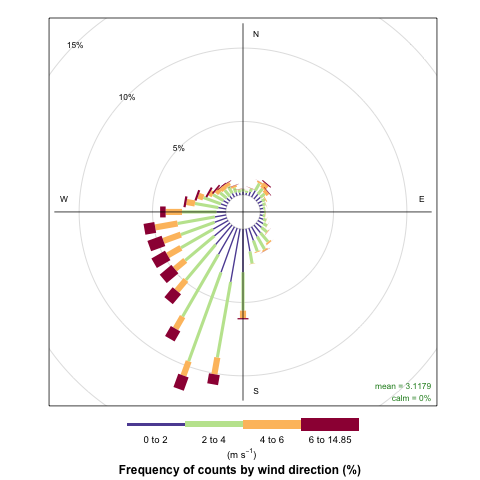
\includegraphics[width=1\linewidth]{figures/Appendix/Windrose/WindRose_Total_medium_peaks.png}
  \caption{}
  \label{WindroseTotal}
\end{subfigure}%
\begin{subfigure}{.5\textwidth}
  \centering
  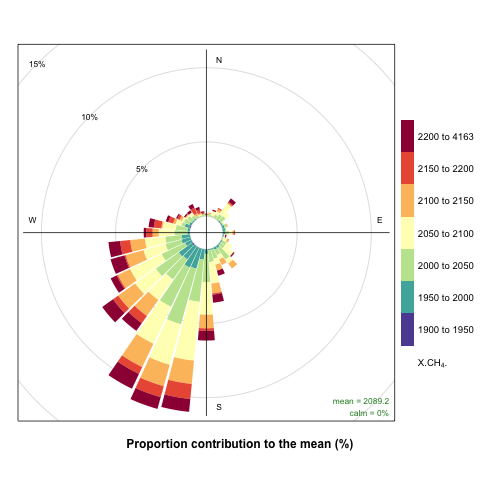
\includegraphics[width=1\linewidth]{figures/Appendix/Windrose/PollutionRose_Total_medium_peaks.png}
  \caption{}
  \label{PollutionroseTotal}
\end{subfigure}
\caption[Windrose and Pollutionrose for total timeline at Geomatikum]{(a) Windrose for the total campaign measured at the Geomatikum. (b) Pollutionrose with wind data measured and CH$_4$ concentration measured at Geomatikum in ppb. }
\label{RoseTotalGeomatikum}
\end{figure}
When  applying the Peak finding algorithm with the strict identification criteria to the wind measurement data, the windrose distribution changes substantially \cref{RosePeaksGeomatikum}. Measurements from the northern with directions are  observed very rarely. Generally, only wind measurements between the South and West are observed regularly. The wind speed is also significantly slower, where most measurements have a speed of 2-4 m/s.\\
The pollution rose plot \cref{PollutionrosePeaks}, in particular, shows that the peaks, especially the high concentration ones, occur in Three distinct directions, South-west and South-South-East. The highest methane concentration peaks above 2600 ppm occurred in wind directions of South-South-West. In this direction, the Elbe is in closest proximity to the Geomatikum. In the South-South-East to the Geomatikum, the city centre with its numerous channels, fleets and small ports is located. This waterbody in this region experiences the effect of the tide strongly.\\
The directions observed in the pollution rose plots are the same as the ones observed in the correlation plot in \cref{MethaneWaterLevel}, correlating the water level and quality with the Methane concentration in the air. This is another indication that the methane observed at the Geomatikum originates at the Elbe.
\begin{figure}
\centering
\begin{subfigure}{.5\textwidth}
  \centering
  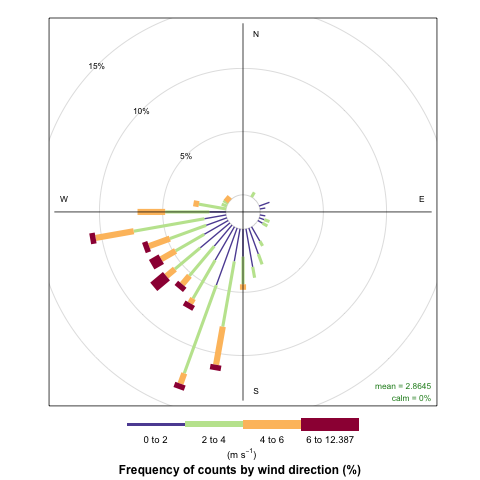
\includegraphics[width=1\linewidth]{figures/Appendix/Windrose/WindRose_Peaks_medium_peaks.png}
  \caption{}
  \label{WindrosePeaks}
\end{subfigure}%
\begin{subfigure}{.5\textwidth}
  \centering
  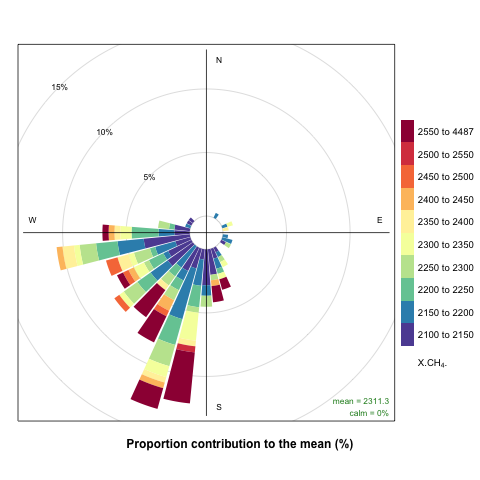
\includegraphics[width=1\linewidth]{figures/Appendix/Windrose/PollutionRose_Peaks_medium_peaks.png}
  \caption{}
  \label{PollutionrosePeaks}
\end{subfigure}
\caption[Windrose and Pollutionrose for total timeline at Geomatikum]{(a) Windrose during CH$_4$ peaks identified with strict criteria measured at the Geomatikum. (b) Pollutionrose for the CH$_4$ peaks with wind data measured and CH$_4$ concentration measured at Geomatikum}
\label{RosePeaksGeomatikum}
\end{figure}

\section{Methane Transport modeling}
\subsection{Source distance estimation}
With the use of the distance estimation model, the distance between the methane peak emission location and the Geomatikum was modelled. The resulting plot can be seen in \cref{DistancePlot}. In this plot, each point represents an individual methane peak with its methane concentration measured at the Geomatikum versus the estimated distance between the emitter and measurement location. The blue line represents a local regression with its standard errors highlighted in dark grey. For this plot, strict peak identification criteria are used. A plot with the identification criteria as described by \cite{Menoud.2021} can be seen in \cref{DistancePlotPaperAppendix}.
\begin{figure}[htbp]
 \centering
 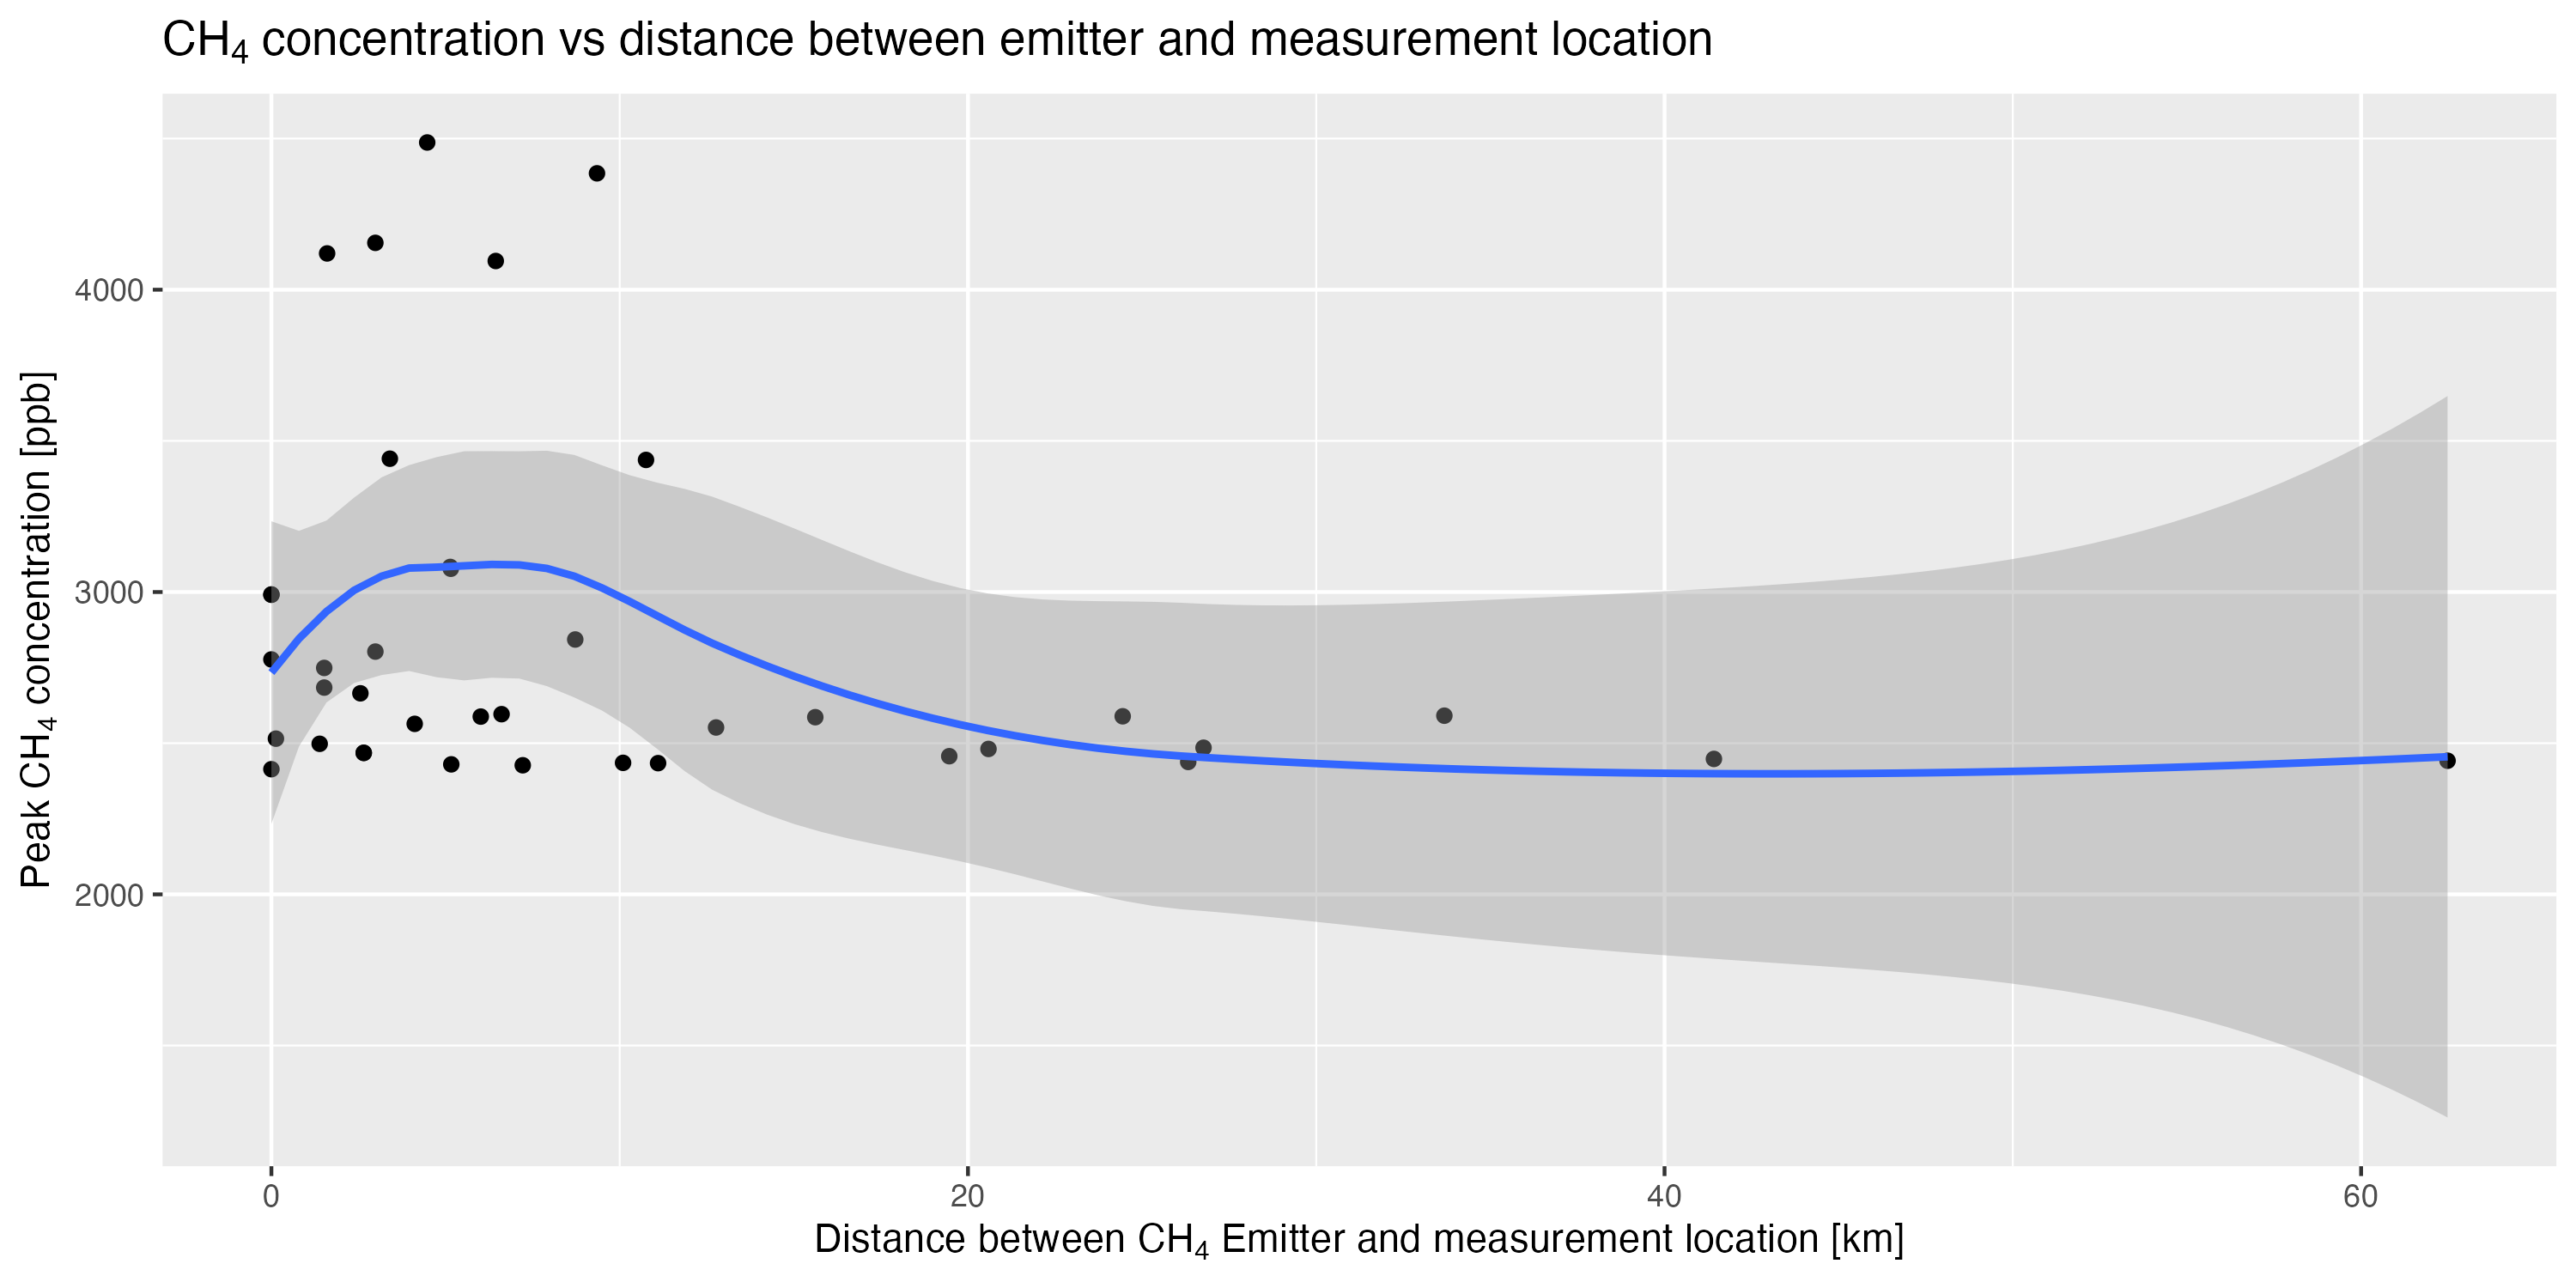
\includegraphics[width=1\textwidth]{figures/Appendix/Transportmodel/14_Low_WL_to_Peak_distance_strict_peaks.png}
 \caption[Distance between estimated emitter and measurement location]{Scatter plot of modelled distance between the estimated emission location and the measurement location at the Geomatikum, against the methane concentration observed at the Geomatikum measured by the CF-IRMS. A local regression line is fitted to the plot (blue),  showing the highest concentration peaks to be emitted at a distance of 5$\pm$3 km. The standard error of the line is shown in dark grey. The peaks were identified using the strict identification criteria.}
 \label{DistancePlot}
\end{figure}
A few details can be observed from the plot. The highest density of peaks is seen between 2 and 10 km distance with a rapidly decreasing density with an increase in distance. A couple of peaks show large distances of up to 60 km away. The distance estimation for those points is most likely not correct as the distance travelled is substantial, and the plume of a  strong and  localized methane emitter would most likely spread considerably over this distance. A geographically large emitter such as the Waddensea is in the 60 km range, and large emissions from this region could, at favourable wind conditions, result in an elevated methane concentration in the air. A possible distance overestimation due to strong winds for a close-by emitter is also possible.\\
The methane concentration measured decreases with the distance. When considering the  local regression line, a peak at a distance of 5 km can be observed. The curve also shows that the peaks estimated to originate further away have a decreasingly lower methane concentration. This curve indicated that the emission location responsible for the high concentration peaks is located at a distance of around 5$\pm$3 km from the Geomatikum. In a 5 km radius of the Geomatikum, most of the Hamburg port, the channels fleets etc., are located. While a 10 km radius includes most of the Waterbodies located in Hamburg.

\begin{comment}
   The distribution changes sustainably when applying the peak identification criteria described in the literature by \cite{Menoud.2021}. While most peaks are estimated relatively close to the measurement location, a high concentration can be measured at a distance of up to 100 km. Some outlier peaks have an estimation of 370 km. The concentration dose again decreases with distance, with the highest concentration under 20 km.
Using this plot, it has to be assumed that the peak identification criteria identified many peaks that don't seem to originate from the Elbe and have a different production mechanism.\\
The plot nether the less helps us to define a boundary for the transport modelling of maximal 60 km from the measurement location. A greater distance would be subject to too many variables.\\ 
\end{comment}

\subsection{Emitter location modeling}
 The transport of the methane has been modelled and is shown in  \cref{TransportmodelStrictPeaks}. In this plot, only the methane peaks identified with the strict identification criteria are modelled. The density distribution represents the probability of the methane emission locations and is shown as a heatmap overlay in the figure.
\begin{figure}
\centering
\begin{subfigure}{.5\textwidth}
  \centering
  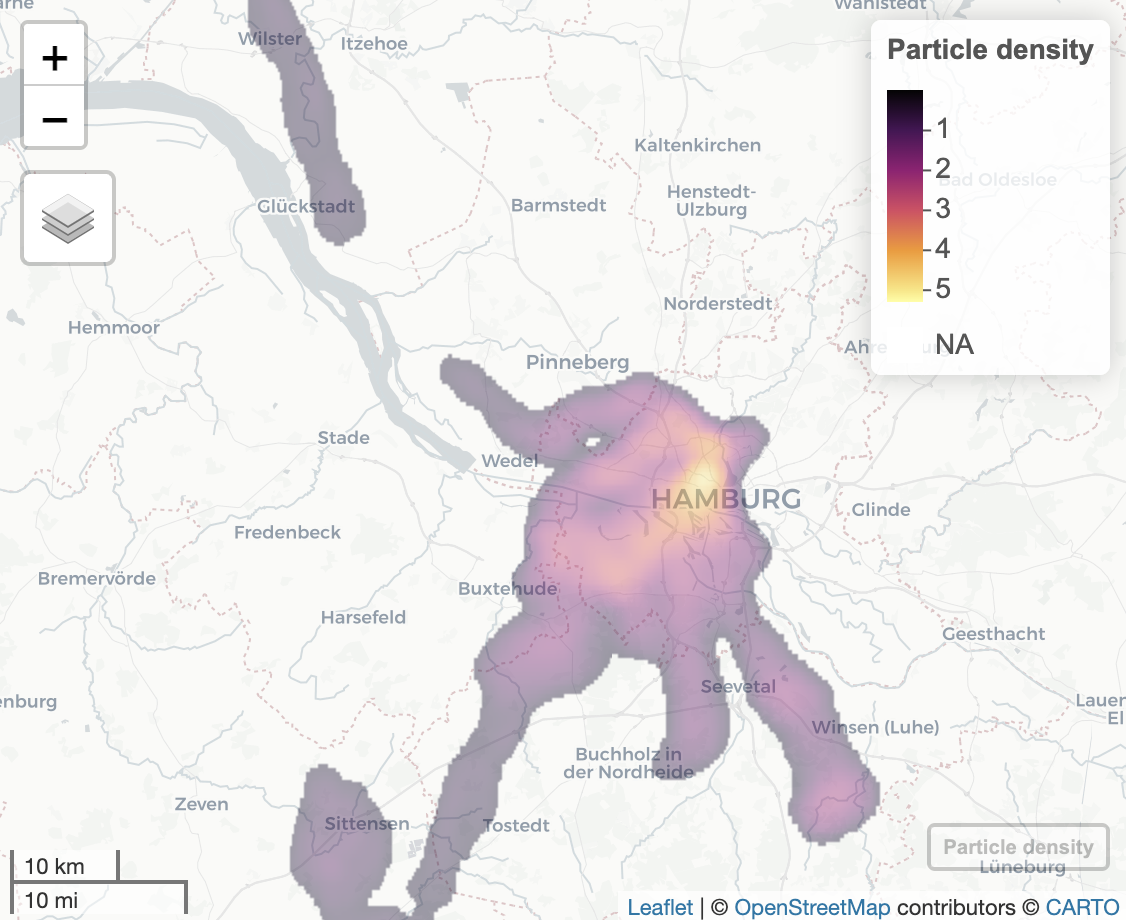
\includegraphics[width=1\linewidth]{figures/Appendix/Transportmodel/10_Emission_Distribution_with_Changing_Measured_Wind_strict_peaks.png}
  \caption{}
  \label{TransportmodelStrictPeaksLrage}
\end{subfigure}%
\begin{subfigure}{.5\textwidth}
  \centering
  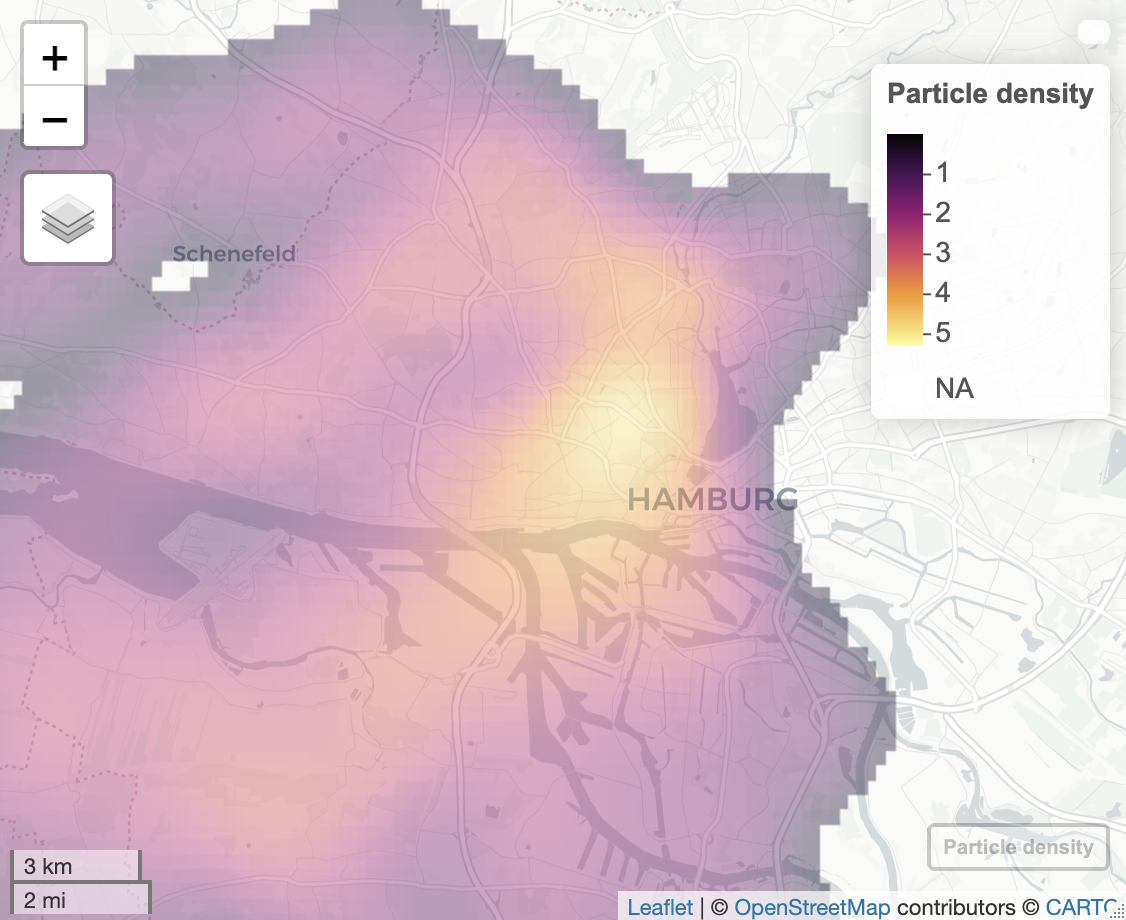
\includegraphics[width=1\linewidth]{figures/Appendix/Transportmodel/10_Emission_Distribution_with_Changing_Measured_Wind_strict_peaks_Zoom.png}
  \caption{}
  \label{TransportmodelStrictPeaksZoom}
\end{subfigure}
\caption[Transport Model]{Map of the partial density for the time-reversed Gaussian plume model. Using strict methane peak identification criteria to select only prominent methane peaks. Wind data was measured at the Geomatikum with 10 min time-averaged values. 1000 Particles released per methane peak with standard deviations of 0.5 m/s and 20°. Heat map overlay representing the particle density at each segment with a logarithmic scale. Figure (b) is zoomed into the Hamburg city region.}
\label{TransportmodelStrictPeaks}
\end{figure}
The plot shows an exceptionally high density in certain inner-city regions. 
The first is in the historic city centre, where the Alster joins the Elbe. This Part of the city has a large, sweet water lake, the Alster, which is relatively shallow. \cite{Maazallahi.2020} and the mobile measurements during the UNEP campaign consistently observed an elevated methane concentration around the Alster. While the enhancements were low in magnitude, they were spread out over a large area around the lake. The Lake and river join the Elbe by locks and controlled water management systems. This region also has many interconnected fleets, historic harbours, and channels freely connected to the river Elbe. Some of them completely dry out for some amount of time during the tide cycle, exposing a deep sediment-rich ground. \\
The second region is the south of Hamburg. The Hamburg port is located in this region, which includes a vast network of channels, contributing rivers, small harbours and some small wetlands. This region also shows an elevated density following the river Elbe upstream land inward. Locks in this region partly control the river and its tidal cycle. Still, most of it is free-flowing and experiences significant water level changes and even running dry in certain areas.\\
The last region of higher density is on the western side. Notably, many tracks follow the Elbe downstream along the Elbe towards the Waddensea. This region experiences the effects of the tide very strongly, with large regions that run dry during low tide. Most notably, some relative wetland regions outside of the city border.\\
This indicates that the origin of the methane peak can be quite far away. Still, the accumulation of methane along the river's entire length in the air is possible. It can produce a high methane concentration in the city with favourable wind conditions. One can also notice that a higher density occurs north of the Geomatikum. But further investigation of the tracks shows that the wind at those peaks is relatively slow and shows a turning wind direction. The tracks also lead to a large wetland region on the Elbe just outside the city bordered on the south-west side of the city.\\
When applying the Peak identification criteria by \cite{Menoud.2021}, identification of a distinct emission region is much more difficult. This is due to the wide range of peak types that are detected with this method. As will be discus in \cref{Keeling}, significantly more Anthropogenic emitters contribute to the smaller peaks. \cref{TransportmodelPaperPeaks} shows that the origin of those peaks, including ones from anthropogenic emitters, is less localised. The region around the Geomatikum shows a high density, with a generally high density in the Hamburg port region to the South and South-West of the Geomatikum. Coincidently this is also the dominant wind direction, as can be seen in \cref{RoseTotalGeomatikum}. The area covered by the tracks and the distance travelled by the particle is generally larger and more uniformly spread in every direction. This probably originates from the more random nature of the peaks occurring at unpredictable times and wind conditions.  
\begin{figure}
\centering
\begin{subfigure}{.5\textwidth}
  \centering
  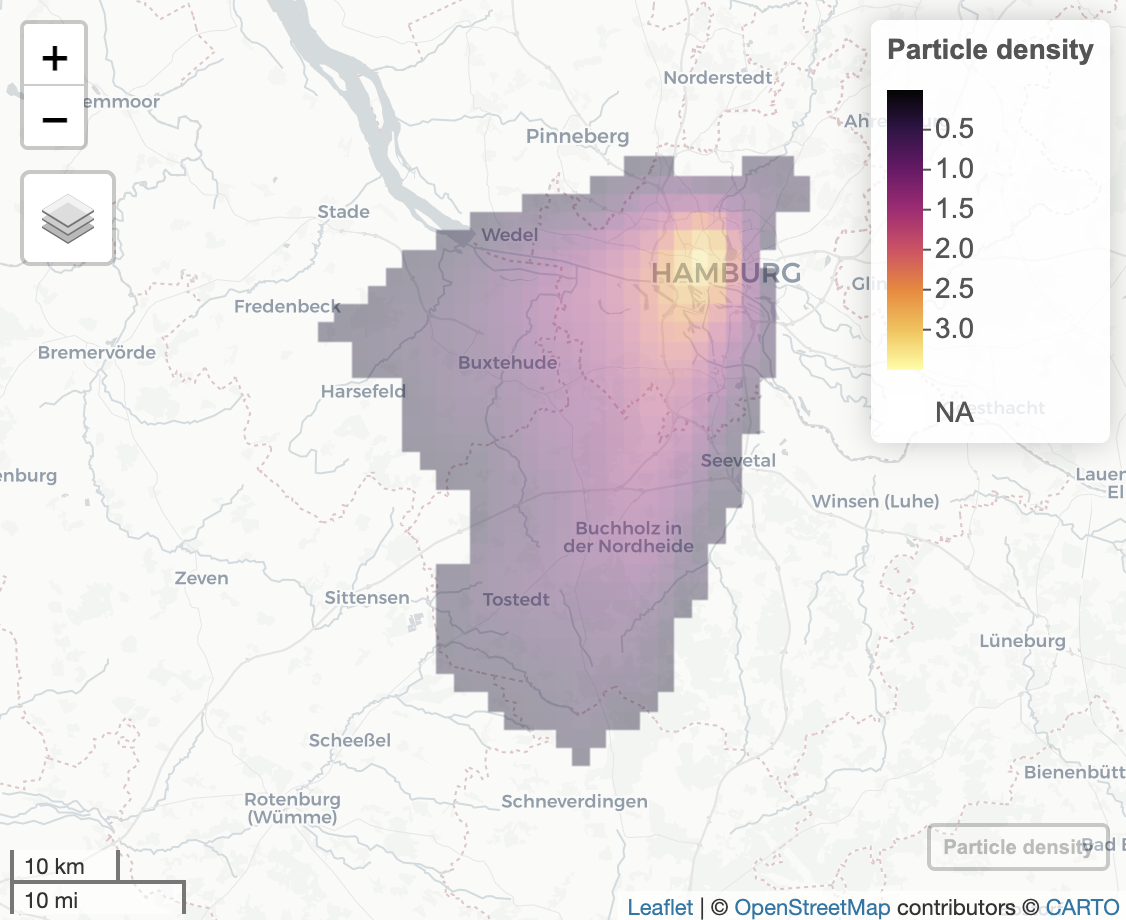
\includegraphics[width=1\linewidth]{figures/Appendix/Transportmodel/10_Emission_Distribution_with_Changing_Measured_Wind_paper_peaks.png}
  \caption{}
  \label{TransportmodelPaperPeaksLrage}
\end{subfigure}%
\begin{subfigure}{.5\textwidth}
  \centering
  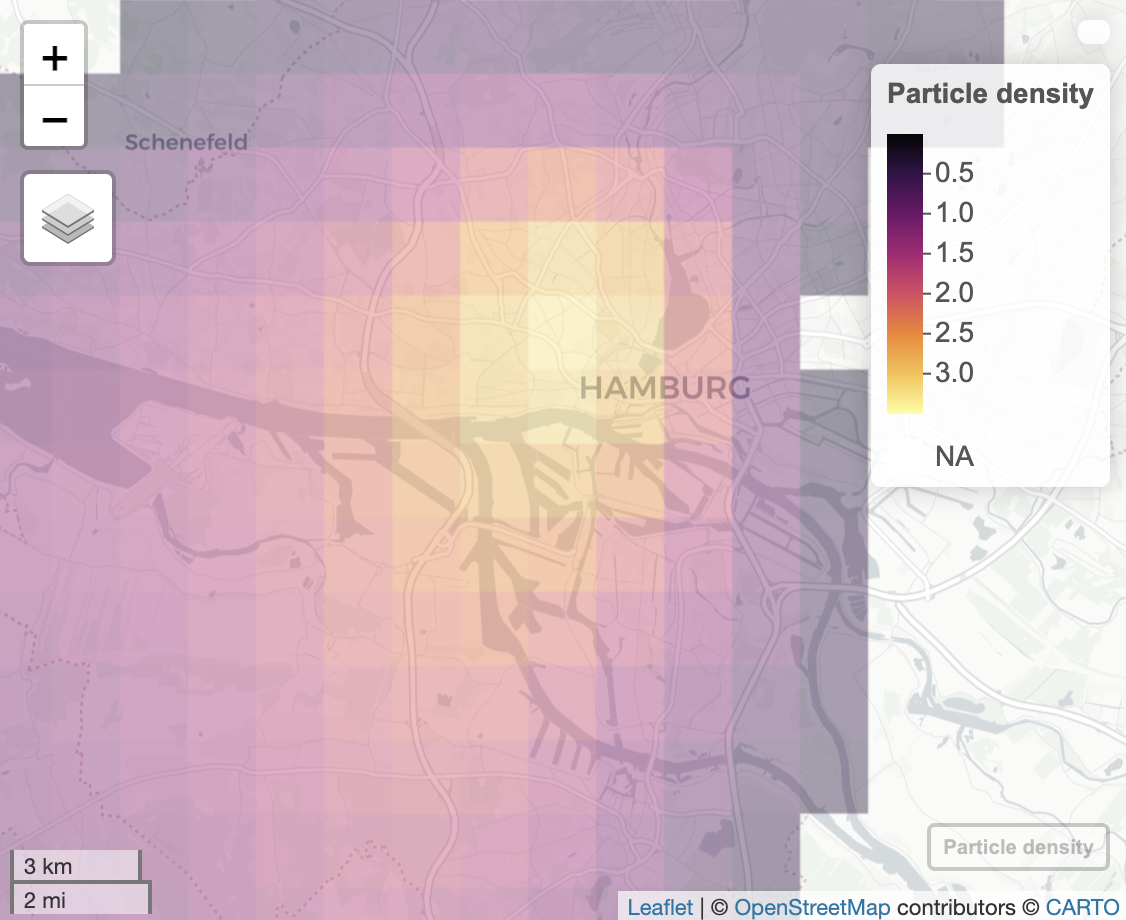
\includegraphics[width=1\linewidth]{figures/Appendix/Transportmodel/10_Emission_Distribution_with_Changing_Measured_Wind_paper_peaks_Zoom.png}
  \caption{}
  \label{TransportmodelPaperPeaksZoom}
\end{subfigure}
\caption[Transport Model with literature Peak identification criteria]{Map of the partial density for the time-reversed Gaussian plume model. Using methane peak identification criteria by \cite{Menoud.2021}. Wind data was measured at the Geomatikum with 10 min time-averaged values. 100 Particles released per methane peak with standard deviations of 0.5 m/s and 20°. Heat map overlay representing the particle density at each segment  with a logarithmic scale.}
\label{TransportmodelPaperPeaks}
\end{figure}

\section{Isotope signature analysis} \label{Keeling}
\subsection{The Keeling plot anlysis}
Using the Keeling method, the methane origin sources were investigated. The complete timeline of the $\delta$13C and $\delta$D CF-IRMS measurements together with the CH$_4$ concentration is shown in \cref{TotalIRMSTimeline}. 
\begin{figure}[htbp]
 \centering
 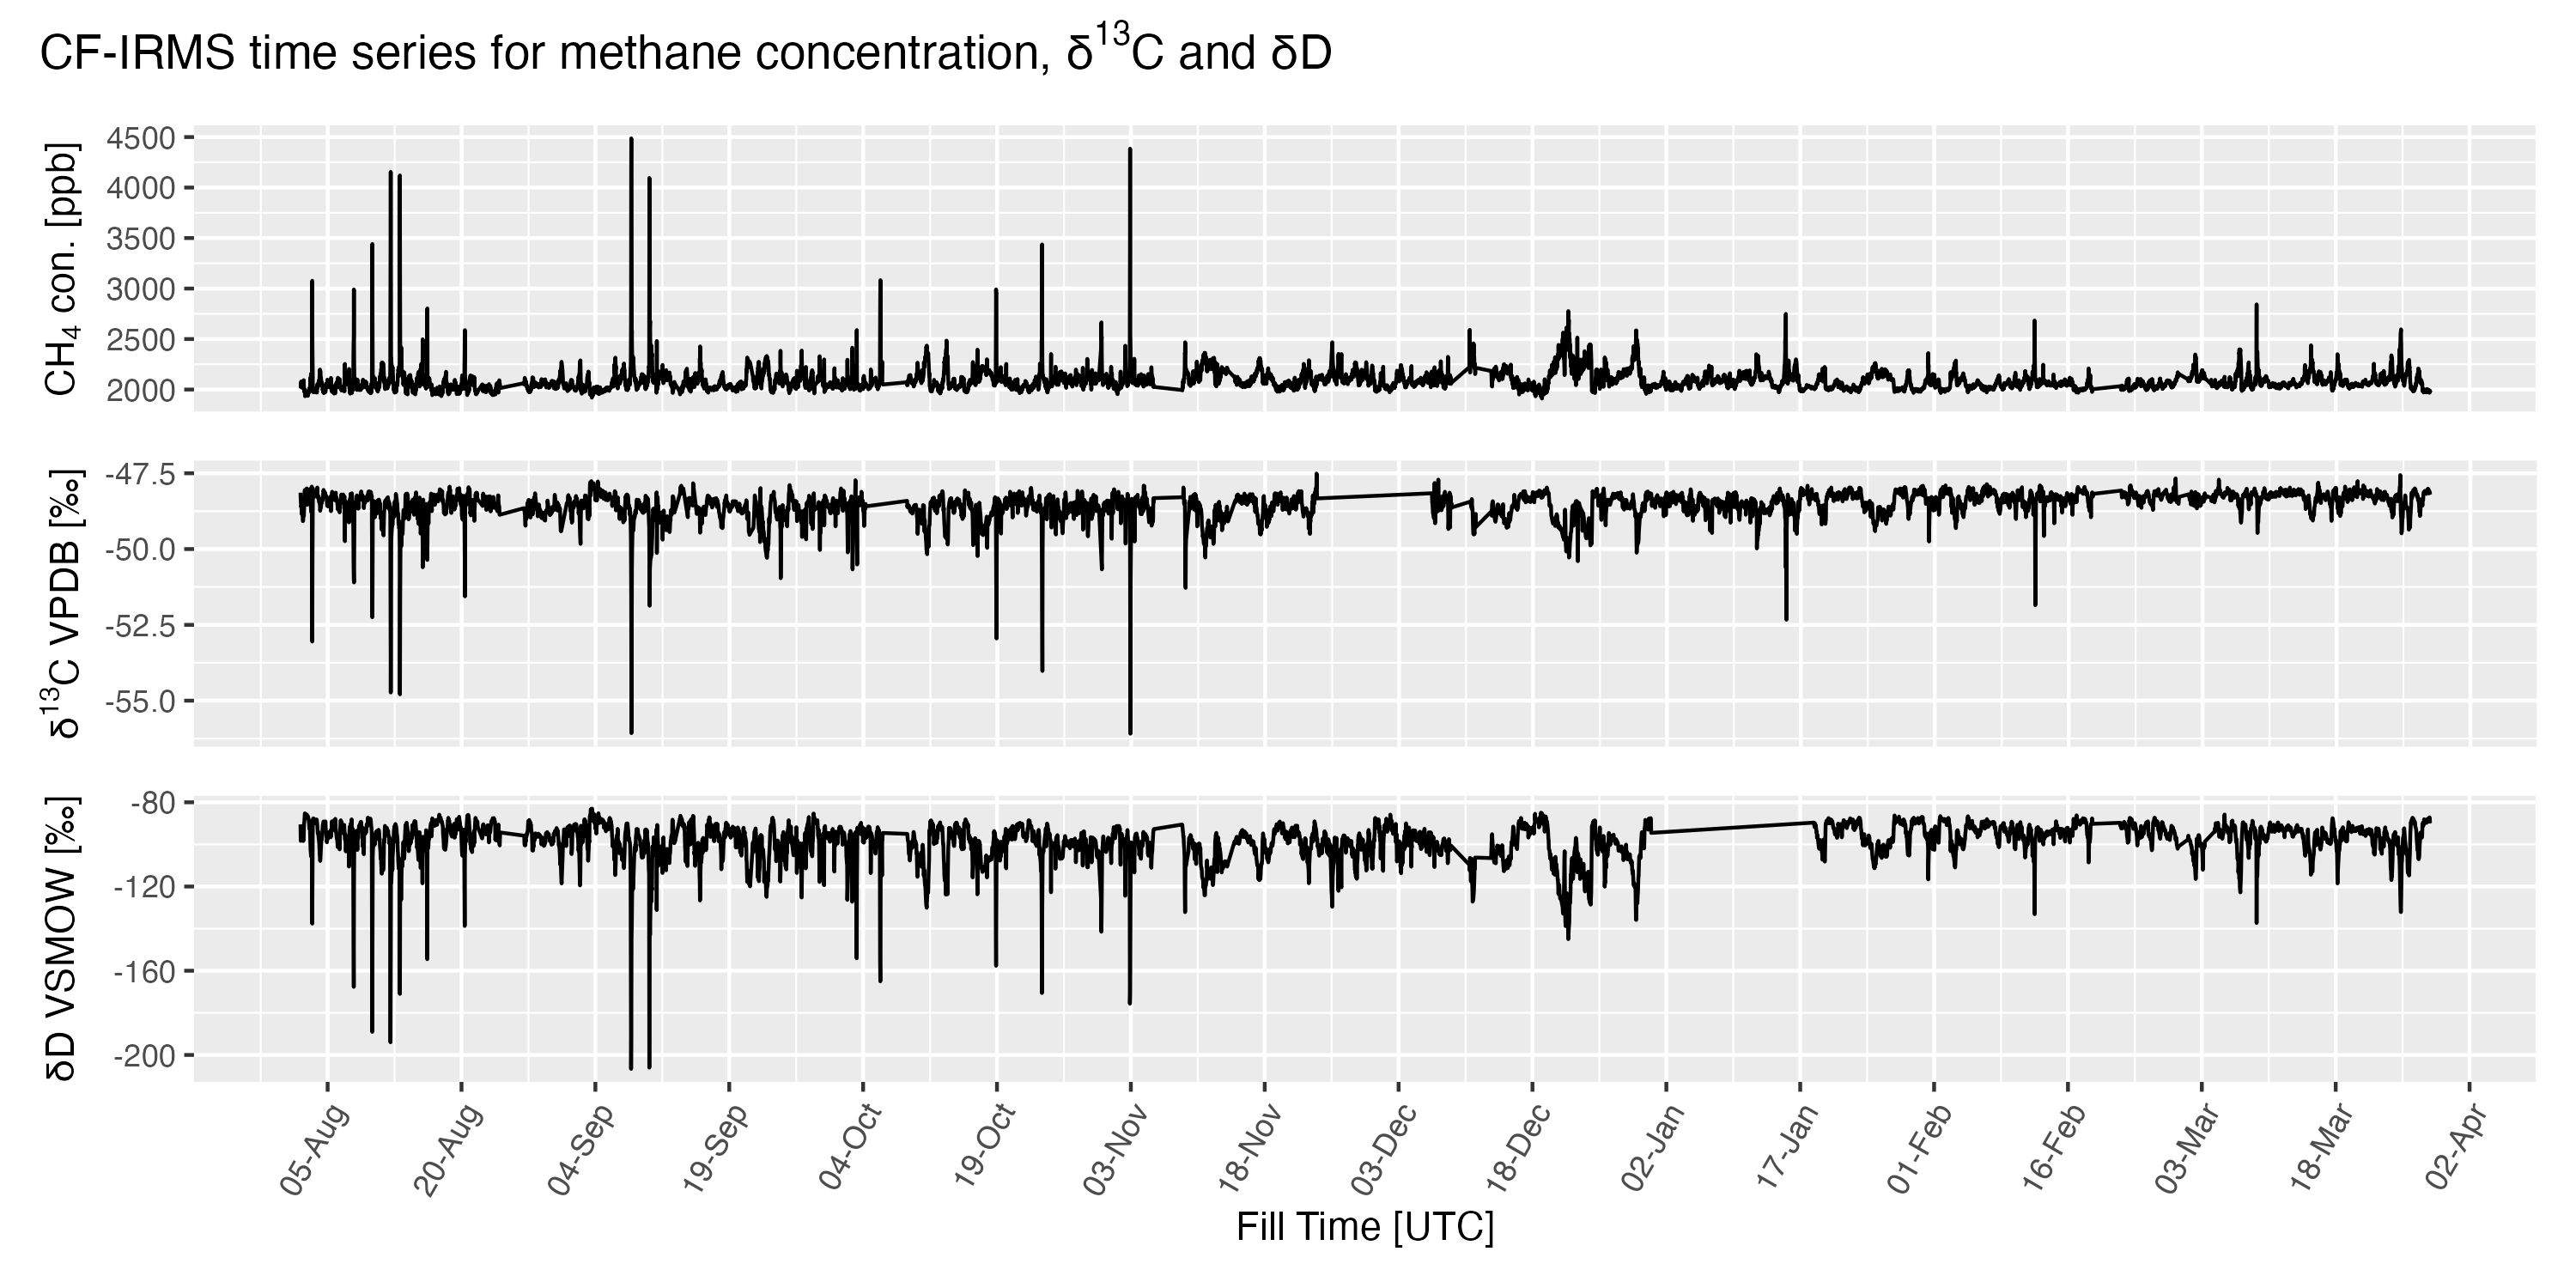
\includegraphics[width=1\textwidth]{figures/Appendix/CH4_Timelines/4_CH4_Total_Timeline.png}
 \caption[$\delta$13C, $\delta$2H and CH$_4$ timeline for CF-IRMS Measument]{Complete timeline of the $\delta$13C, $\delta$D and CH$_4$ concentration measured by CF-IRMS at Geomatikum from 1.08.2021 to 1.04.2022}
 \label{TotalIRMSTimeline}
\end{figure}
By using this complete timeline, the Keeling plot approach was deployed, and the resulting plots are shown in \cref{TolalKeelingPlot}. The isotopic signature for Carbon-13 was calculated to be $\delta$13C = -57.7$\pm $0.1$\permil$ and for Deuterium to be $\delta$D = -290.5$\pm $0.8$\permil$.  Comparing those results to the database values show that the dominant methane production mechanisms during the total campaign time in Hamburg were thermogenic and microbial CO$_2$ reduction. In particular, wetland, agriculture, and waste. Fossil fuel and other anthropogenic sources play a minor role in the composition of the methane mixture. This is surprising as Hamburg has a significant amount of heavy industry, including fossil fuel refinery, chemical industry, shipping, energy production etc.
\begin{figure}[htbp]
 \centering
 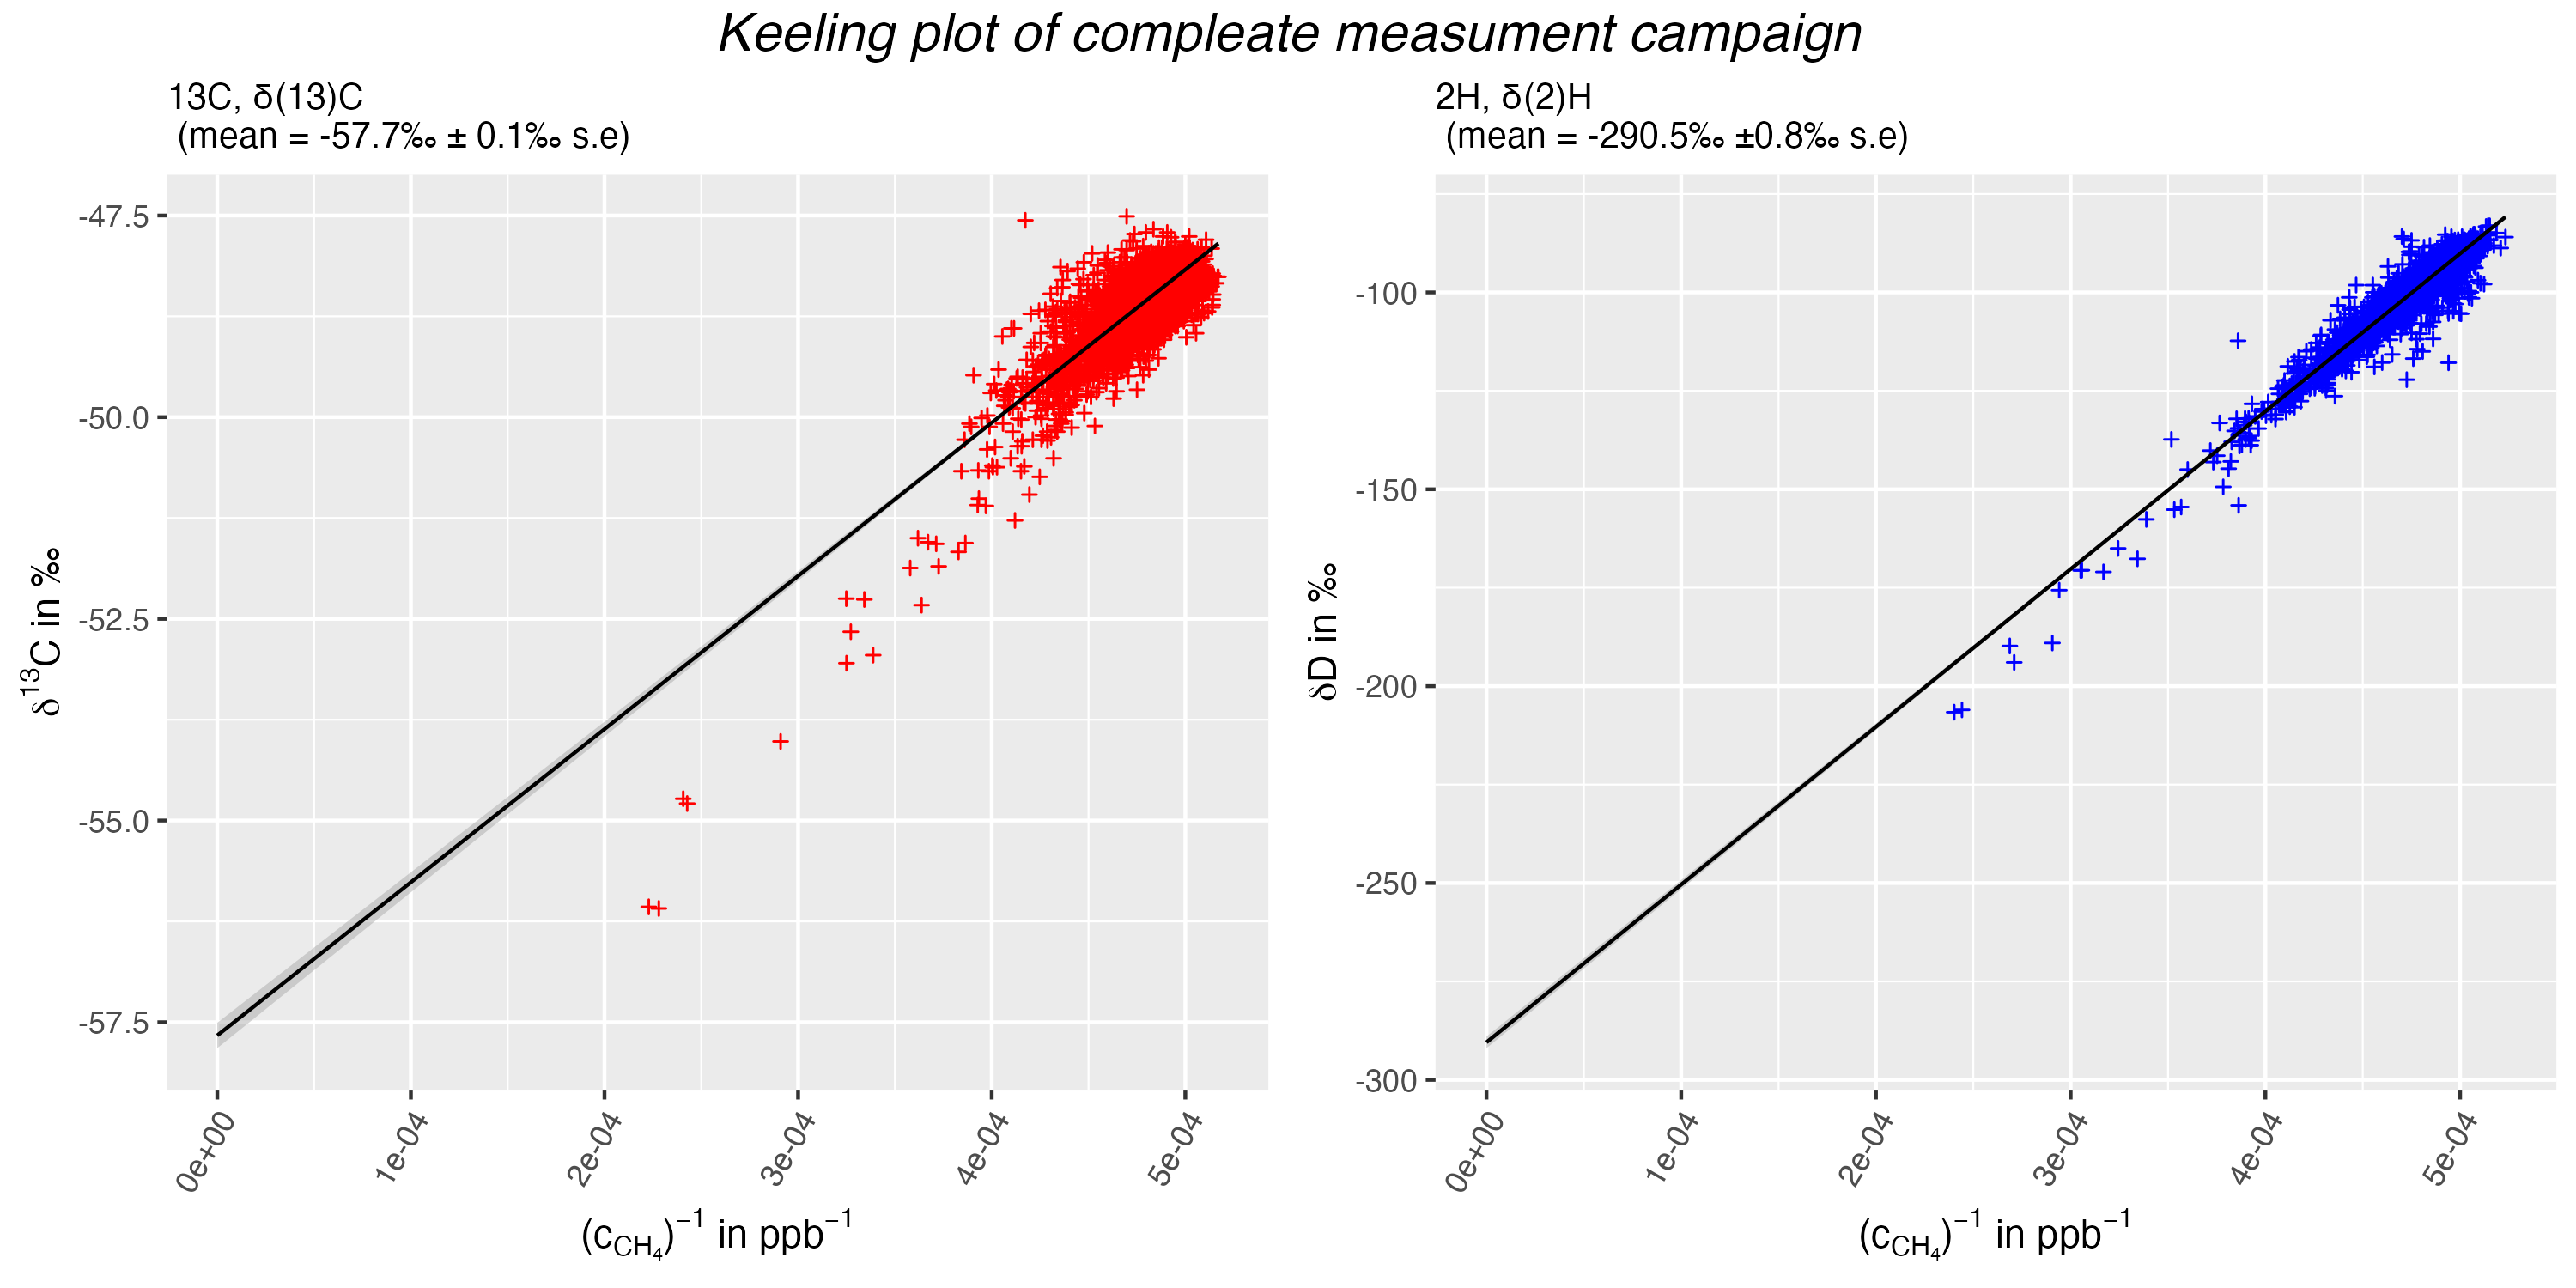
\includegraphics[width=1\textwidth]{figures/Appendix/Keeling/11_Keeling_Plot_Total_medium_peaks.png}
 \caption[Keeling Plot for total CR-IRMS measument]{Keeling Plots of Carbon-13 and Deuterium in methane measured at the Geomatikum from 1.08.2021 to 1.04.2022. The resulting isotopic signatures $\delta$13C = -57.7$\pm $0.1$\permil$ and $\delta$D = -290.5$\pm $0.8$\permil$}
 \label{TolalKeelingPlot}
\end{figure}
On the other hand, this is expected, as the surrounding countryside has significant ecocultural use, including cattle farms and large wetland and marshland areas nearby. This also includes the vast Waddensea of the German bight near the city. This Waddensea region lay upwind in the dominant wind direction to the west.\\
By applying the peak finding algorithms to the methane measurements data exclusively, the methane peaks were investigated. Here it is focused on the strict identification criteria. The Keeling plots for the identified peaks are shown in \cref{PeaksKeelingPlot}. The Keeling method shows isotopic signature for  Carbon-13  to be $\delta$13C = -60.3$\pm $0.2$\permil$ and for Deuterium to be $\delta$D = -298$\pm $2$\permil$. This indicates methane production mechanisms are much more evident in the microbial CO$_2$ reduction region and less in the thermogenic, shifting this more clearly into the wetland region, while less likely to originate from waste and agriculture. The Keeling method points toward the origin of the methane peaks due to biogenic mechanisms in the river Elbe, its contributors and the wetlands at its riverbanks.
\begin{figure}[htbp]
 \centering
 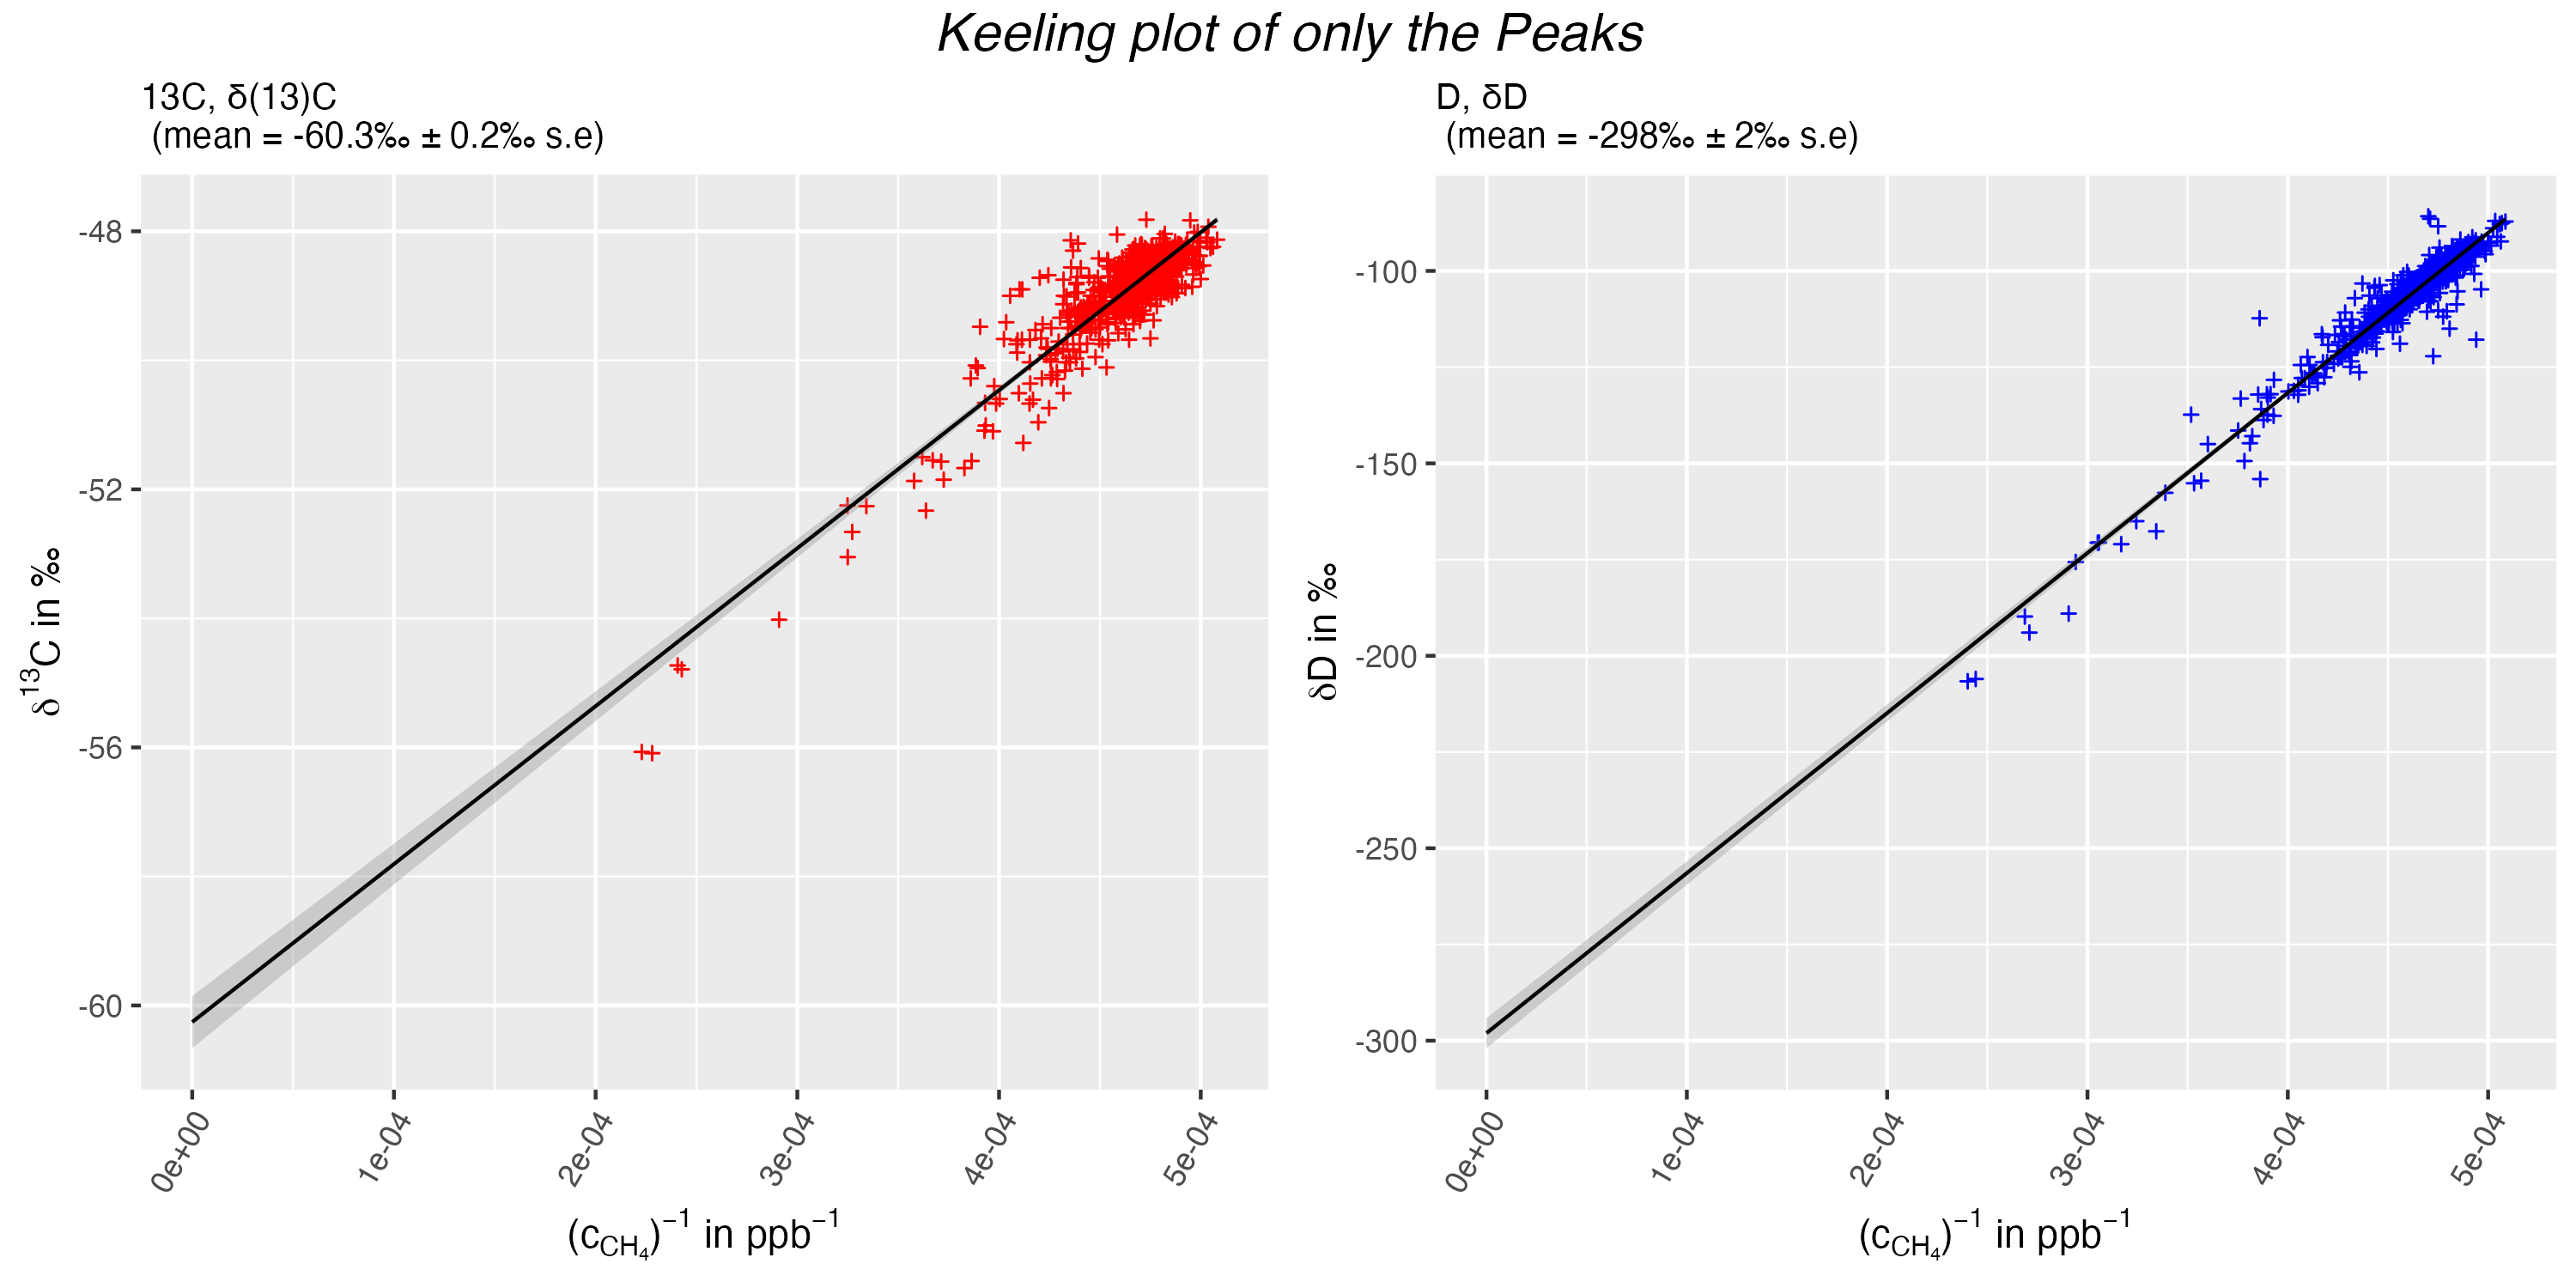
\includegraphics[width=1\textwidth]{figures/Appendix/Keeling/11_Keeling_Plot_Peaks_medium_peaks.png}
 \caption[Keeling Plot for CH$_4$ peaks in CR-IRMS measument]{Keeling Plots of Carbon-13 and Deuterium in methane peaks measured at the Geomatikum from 1.08.2021 to 1.04.2022. Strict peak identification criteria were used that only selected the prominent methane peaks. The resulting isotopic signatures $\delta$13C = -60.3$\pm $0.2$\permil$ and $\delta$D = -298$\pm $2$\permil$}
 \label{PeaksKeelingPlot}
\end{figure}
Using the wind direction makes it possible to take an even closer look at the methane emission type depending on its estimated origin location. This is done in the dual isotope plot seen in \cref{DualIsotiotopePlots}. Here a Keeling analysis for every wind direction is done within 10° bins. Each point has an error bar corresponding to its standard deviation. The point colour indicates the wind direction in regard to the North (Blue) and South (Red) wind directions. The wind directions, West and East are not considered in this plot for simplification. The Highlighted coloured areas indicate the fundamental methane production method (Microbial CO$_2$ reduction (Yellow); Microbial fermentation (Pink); Thermogenic (Dark Green) and Abiotic (light blue)). The coloured boxes show particular emitter types (Fossil fuels and non-industrial combustion (Red); Agriculture (Green); Waste (Purple); Other anthropogenic sources (dark blue); Natural wetlands (Black)). The reference database used in this dual isotope plot for the highlighted segments is from \cite{Menoud.2021}.\\
In the dual isotope plot considering the total measurement time series \cref{DualIsotiotopeTotal}, one can identify a difference in isotope signature and origin type by the wind direction. For the entire measurement series, one can see that the signature shifts to the abiotic production type for general northern wind directions, hence towards fossil fuels and other anthropogenic sources. As considerably fewer wetlands are present in this region, and many residential areas lay there, one can assume that this shifts the methane mixture towards fossil fuels. Most likely due to unburned methane from heating and cooking, leakage in the gas grid and energy generation plays a significant role in the composition of the methane mixture \cite{Lebel.2022}, \cite{Dietrich.2023}. Confirming the observations made by \cite{Maazallahi.2020} who focused on ground-based mobile measurements in the northern region of Hamburg identifying numerous methane leaks ordination from the leaks in the gas grid.
\begin{figure}
\centering
\begin{subfigure}[b]{1\textwidth}
   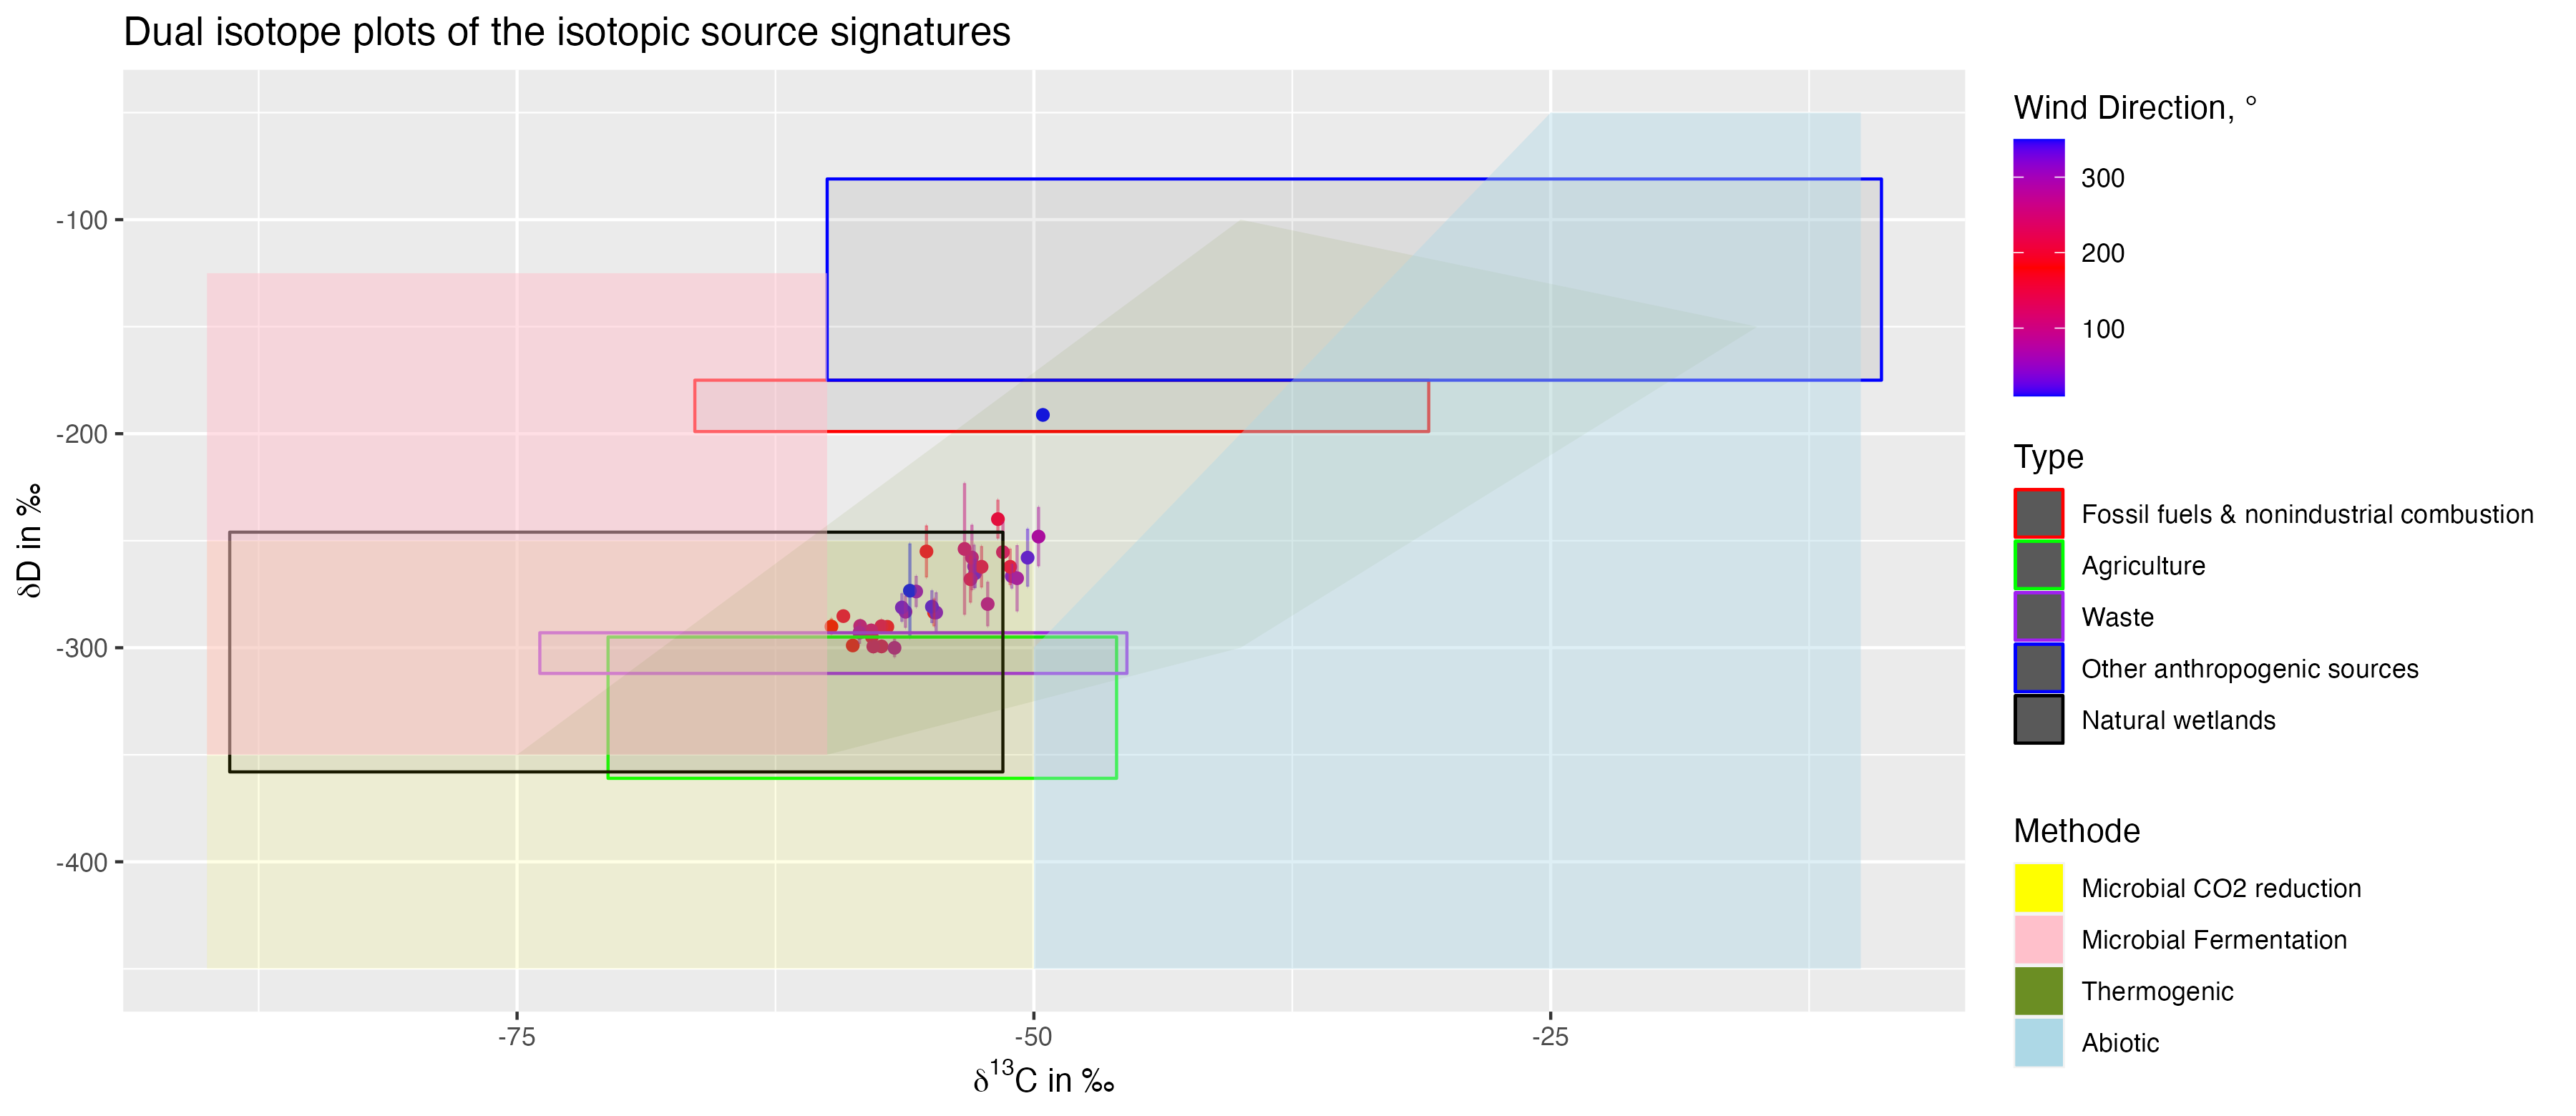
\includegraphics[width=1\linewidth]{figures/Appendix/Keeling/12_Keeling_Total_Wind_medium_peaks.png}
   \caption{}
   \label{DualIsotiotopeTotal} 
\end{subfigure}

\begin{subfigure}[b]{1\textwidth}
   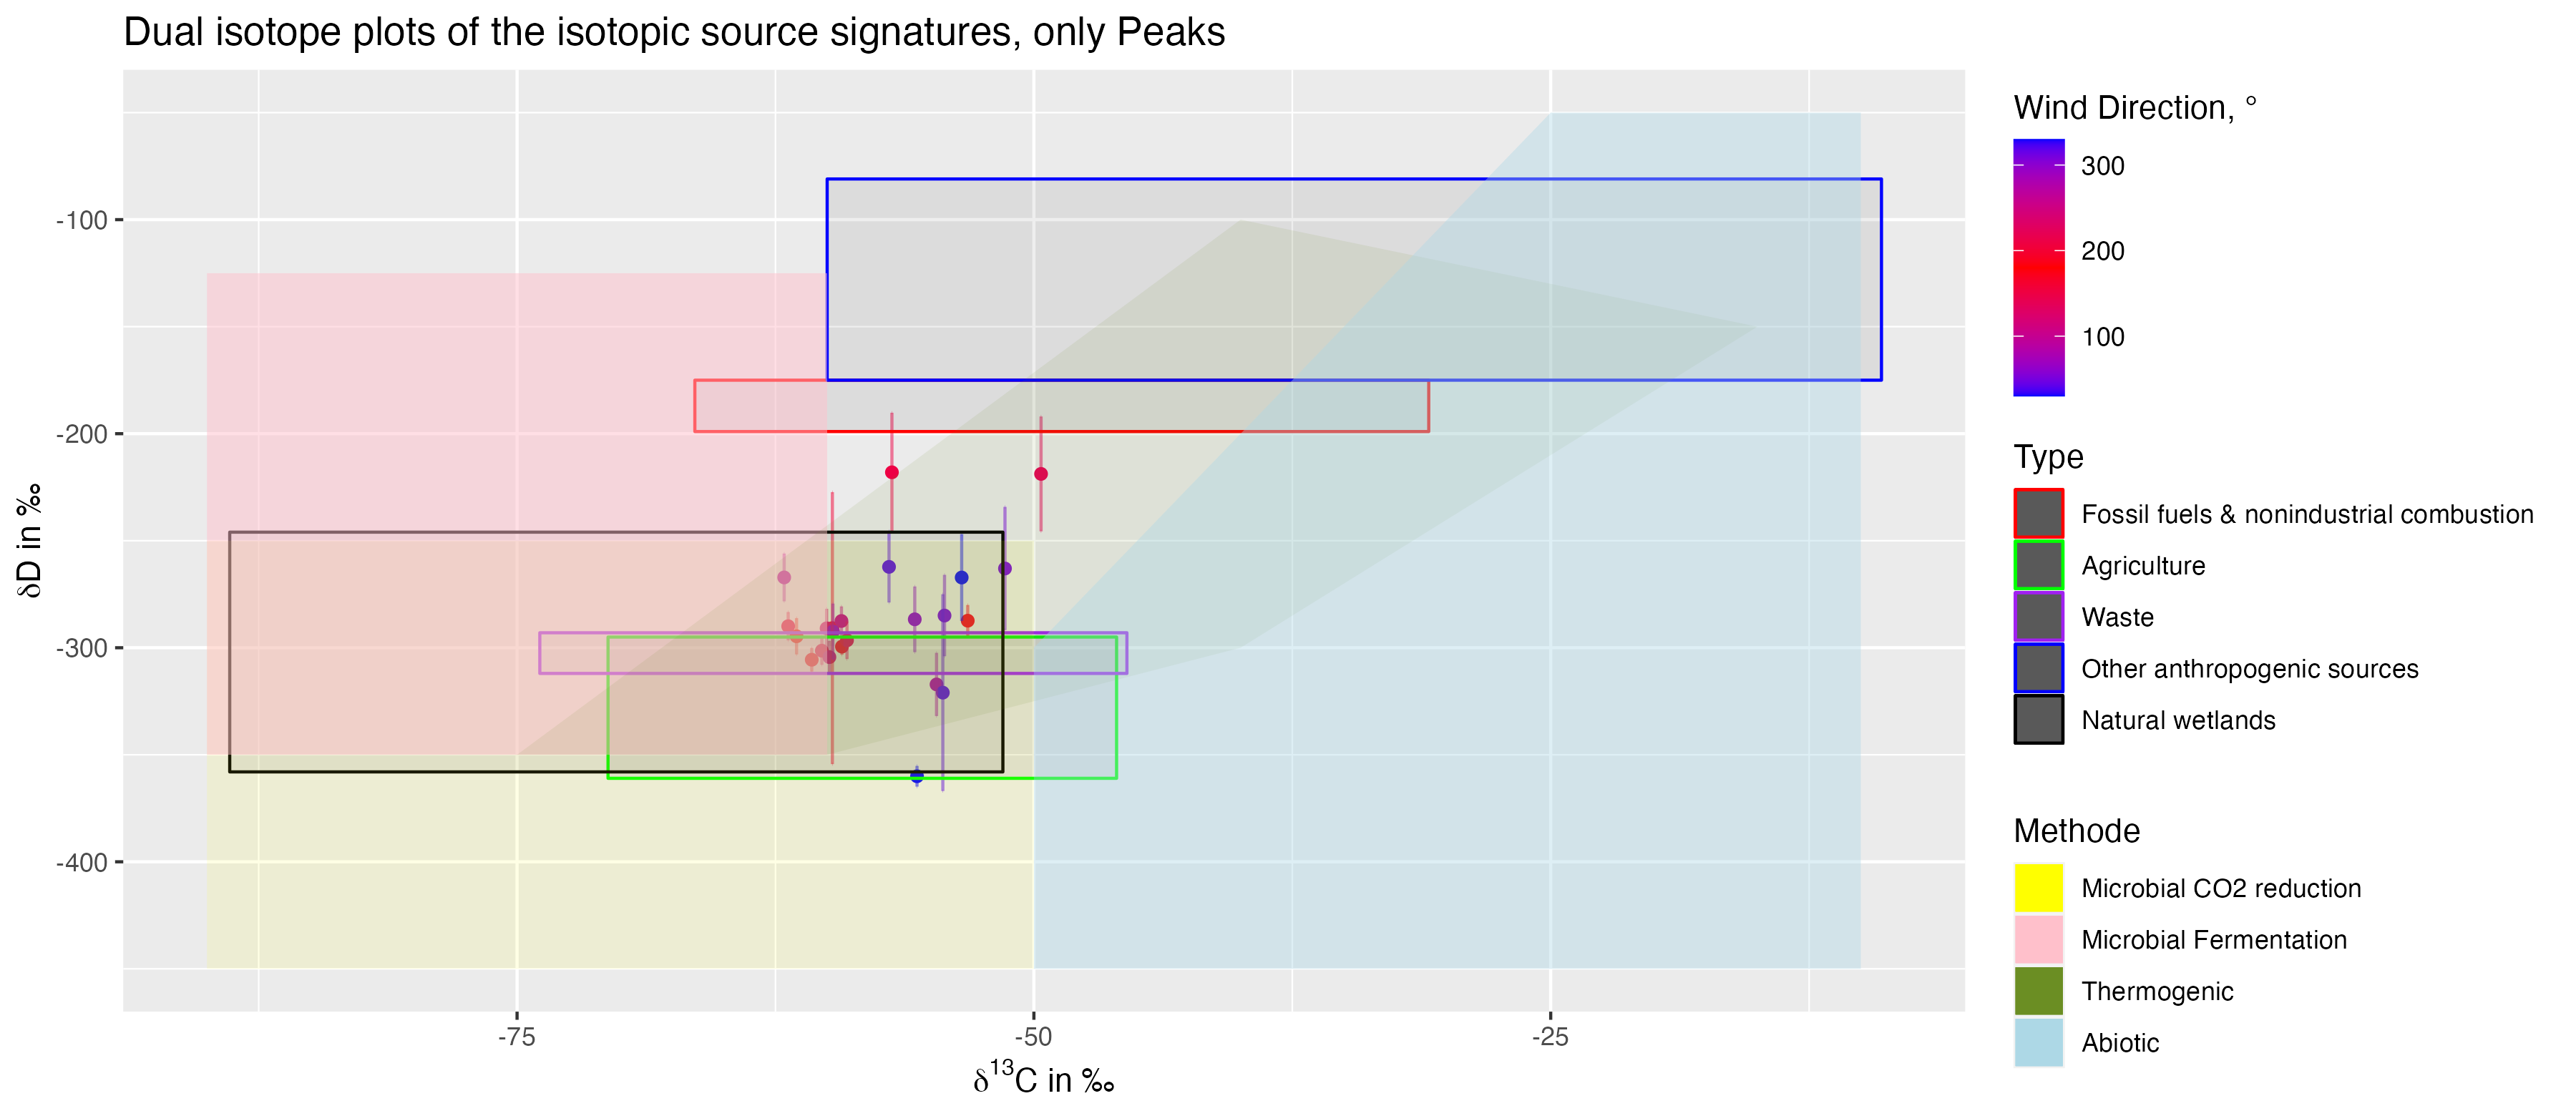
\includegraphics[width=1\linewidth]{figures/Appendix/Keeling/12_Keeling_Peaks_Wind_medium_peaks.png}
   \caption{}
   \label{DualIsotiotopeMediumPeaks}
\end{subfigure}
\caption[Dual isotope plot with strict peak identification]{Dual isotope plot for CF-IRMS measurement for 10° wind direction represented as point colour(blue towards North, red toward South) with highlighted production mechanism (coloured highlight) and source type (coloured boxes). Error bars show one SD. \cref{DualIsotiotopeTotal} shows total time series, \cref{DualIsotiotopeMediumPeaks} shows only peaks selected with strict identification criteria}
\label{DualIsotiotopePlots}
\end{figure}
For the southern and western directions, the methane signature is quite strong in the microbial CO$_2$ reduction region, pointing out that the most significant contributors to this methane mixture are wetlands, agriculture and waste. At the same time, waste can be more or less eliminated due to the absence of large landfills in the region. As mentioned previously, this is expected due to its geographical and biological features, together with the strongly agriculturally use of the region. What is surprising is the minor effect of anthropogenic sources, like fossil fuel and industry, as this region is heavily used.\\
The same analyses have been done for the methane peaks, as seen in the dual isotope plot, \cref{DualIsotiotopeMediumPeaks}. Here, it has to be noted that not all wind directions had sufficient peaks to create a statistically meaningful keeling analysis. The dual isotope plot indicates a wetland and agricultural origin for the remaining wind directions. Pointing again toward a biogenic origin in the river Elbe and its wetlands.
\begin{comment}
    A study on a river estuary at the border between Belgium and the Netherlands by Jacques et al. (2021) found a comparable signature for δ13C (between-25.2‰ and-65.6‰),howeveramoreenrichedsignatureforδD(between+101‰ and-212‰). δDsignaturesof down to -260 ‰have been measured by Martens et al. (1999) for gassy sediments in an estuary in Germany. The slightly less enriched δD signature measured in this study suggests that the unknown source in Hamburg could be a mix of several different biogenic (microbial) sources. One of these could be a large natural CH4 source, like for instance the river or wetlands that emit in Hamburg (See also section 3.1). The river flow in the city area is however also influenced by anthropogenic activity (harbor traffic, wastewater, etc.) which could contribute to lower δD values.
\end{comment}

\section{FTIR total column analyse}
The FTIR measurements suffered from technical limitations that restricted the measurement time of the sensor network. In addition to the inability to measure during the night, the weather severely disturbed the measurements. During the relatively short period between 27.07.2021 and 09.09.2021, much precipitation and consistent cloud cover were observed. For the Bayesian inversion to operate, at least two stations must operate uninterrupted for an extended time. To find good days for the Inversion, a series of prefilters were applied, which are as follows:
\begin{enumerate}
  \item Physical properties of the measurements
  \begin{itemize}
    \item solar elevation
    \item absolute solar intensity
    \item solar intensity variation during an FTIR scan
  \end{itemize}
  \item statistical removal of outliers and measurement periods with too few data points
    \begin{itemize}
     \item At least two stations measured at the same time
     \item More than 5 hours per day per station
  \end{itemize}
  \item measurements are averaged using a 10-minute moving average
\end{enumerate}
This resulted in only nine usable days out of a 43-day campaign. \\
The inversion model estimated a total annual emission for the uncorrected TNO GHGco inventory and the mobile measurement updated inventory. The emissions sources were also segmented into natural and anthropogenic. With the TNO GHGco inventory, the emissions by the natural (including the river)and anthropogenic sources added up to  6300 $\pm$ 3500 kg h$^{-1}$, and with the updated inventory to 6300 $\pm$ 4100 kg h$^{-1}$ for the total modelling domain. This domain included a significant area surrounding the city and can be seen in \cref{ModdelingDomain}. For the natural sources, which include the Elbe, the model estimated hourly emission of 1900 $\pm$ 1000  kg h$^{-1}$ for the TNO GHGco inventory and 1900 $\pm$ 1000  kg h$^{-1}$ for the updated inventory \cite{Forstmaier.2023}. This is a significant amount of the total emissions in the domain. A considerable amount of the modelled methane emissions can be attributed to the Elbe, its contributors and riverbanks, marshland and wetland surrounding the River.

\begin{figure}[htbp]
 \centering
 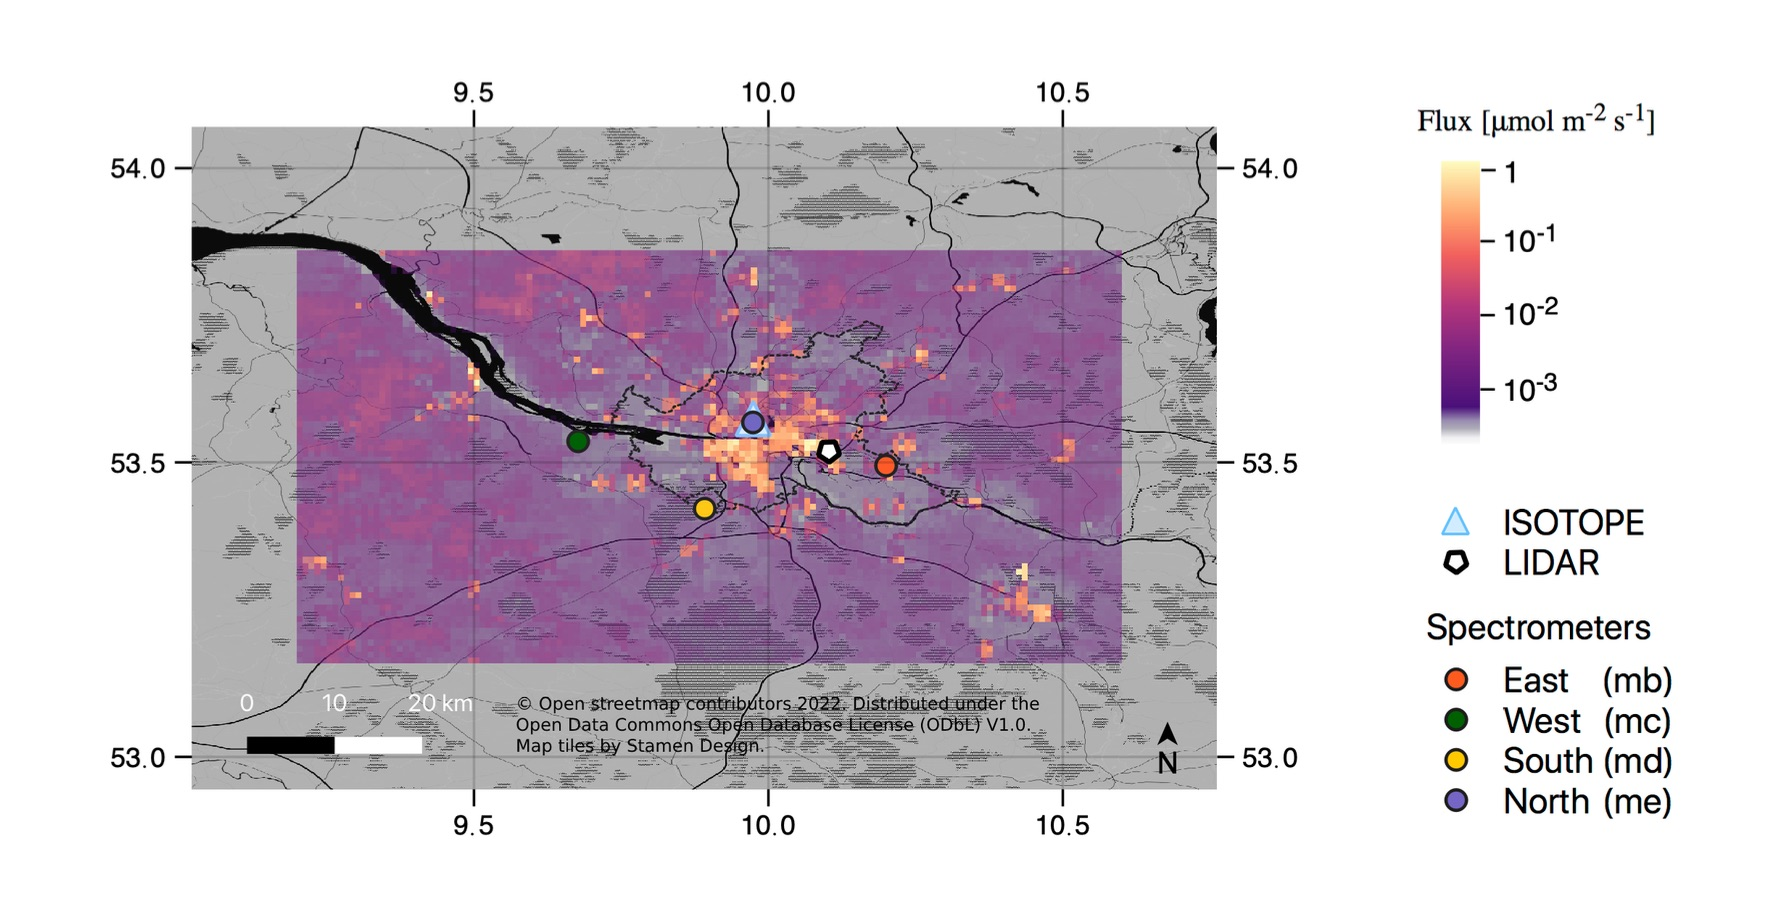
\includegraphics[width=1\textwidth]{figures/Appendix/Map/ModelingDomainFTIR.jpg}
 \caption[Modeling domain]{ Modeling domain used in the Bayesian inversion with the Prior TNO GHGco emission inventory. No Corrections for the mobile measurements and the Elbe. The locations of the FTIR Spectrometers, wind lidar and CF-IRMS during the campaign are shown. The city borders of Hamburg are marked in black. \cite{Forstmaier.2023}}
 \label{ModdelingDomain}
\end{figure}

\subsection{Total column methane peaks}
To identify methane peaks that can be linked to the tidal cycle of the Elbe, individual sensor stations needed to measure uninterrupted for an extended amount of time. A low water cycle also needed to align with this measurement window. As with the CR-IRMS measurement, the wind conditions also needed to be favourable to transport a plume to the observation column.\\
Multiple peaks that appear to originate from the water level dropping in the Elbe could be identified by manually filtering the total column measurements and the water level measurements. For those peaks, the transport model showed that the wind direction and speed were favourable for emission from the river and its surroundings to be measured at the sensor locations. \\
Peaks suggested to originate from the Elbe were mainly observed from the stations at the Geomatikum (North (me)) and Jork (West (mc)). The Geomatikum (North (me)) station showed that the concentration and occurrence of methane peaks measured by the FTIR spectrometer were relatable to the CR-IRMS measurements. \\
The Jork (West (mc)) station was located relatively close to the Elbe, to its South, which is upwind of the dominant wind direction of Hamburg. Methane peaks, likely originating from the Elbe, were still observed occasionally at wind directions from the North \cref{FTIRWLJork}. The remaining stations at Rosengraten (South (md)) and Bergedorf (East (mb)) were quite far from the Elbe, both in opposite directions from the predominant wind direction. At favourable wind directions, elevated concentrations could be observed \cref{FTIRWLRosengarten}, but a clear link to the Elbe could not be made due to the strong influence of the city and the large distances to the Elbe.\\
An example of a methane peak that is assumed to originate from the dropping water level of the Elbe is seen in \cref{FTIRWL}. The measurement was performed at the Geomatikum on 06.08.2021. The wind conditions at the Geomatikum  were suitable for a plume to be transported to the measurement location. The peak reaches its maximum at the lowest water level of the Elbe. When comparing the FTIR measurements to the CF-IRMS measurements, the same methane peak can be observed with both measurement techniques. A clear distinction between the two measurements is the measured concentration. While the FTIR measurement shows a peak of 1903 ppb from an 1896 ppb background, the CR-IRMS measurements show a peak of  2120 ppb from a 1995 ppb background. The smaller concentration at the peak in the FTIR measurement is due to the averaging over the total air column instead of a surface-level in situ measurement.
\begin{figure}[htbp]
 \centering
 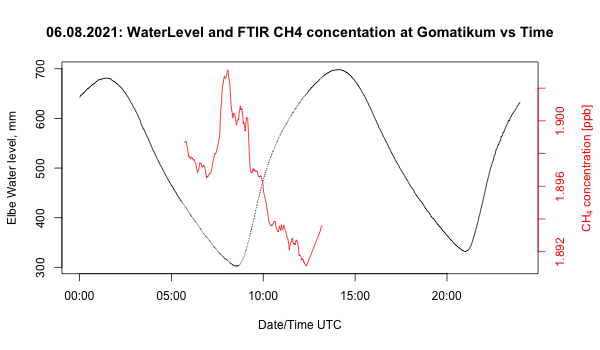
\includegraphics[width=1\textwidth]{figures/Appendix/FTIR/15_Basic_Plot_CH4_Wl_FTIR.png}
 \caption[FTIR methane concentration and water level height]{Plot of the total column methane concentration measured at the Geomatikum (Red line), overlayed with the Elbe water level measured at St. Pauli (black line). The measurements were performed on 06.08.2021.}
 \label{FTIRWL}
\end{figure}
Similar peak observations can be observed over the short FTIR measurement campaign. Generally, no significantly larger peaks were observed with the FTIR approach, as seen in the CR-IRMS timeline, where peaks reached a concentration over 4000 ppb. The FTIR network could not measure simultaneously during those large peaks due to sunlight availability or weather conditions.  Unfortunately, reliable statistical correlations, as can be seen with the CF-IRMS measurements, could not be observed with the FTIR approach. The spotty measurement intervals don't allow for reliable peak identification, and the few continuous measurements are insufficient for a reliable statistical correlation. 


\chapter{Conclusion and Discussion}
\label{chap:ConAndDis}

%\section{Conclusion}
The long-term high temporal resolution CF-IRMS measurements showed high-concentration methane peaks. Those peaks were observed for the total measurement campaign over eight months. The FTIR network measurements performed for a shorter time period also were able to observe those peaks at favourable weather conditions. Due to additional measurement limitations of the FTIR sensor network, a continuous measurement was not possible, excluding measurements during the night and in cloudy conditions. This resulted in only very few instances where methane peaks could be observed with both measurement approaches simultaneously, prohibiting a detailed direct comparison between the two approaches.\\
A Keeling plot analysis of the CF-IRMS time series showed an isotopic signature of the methane in the air that was strongly influenced by natural emitters. While measurements performed during northern wind directions were shifted more to emission types that are observed with Anthropogenic emitters. To the north of the measurement site, mostly residential areas are located. Previous studies in this region showed a high methane enrichment with numerous plumes, most likely originating from natural gas infrastructure leakages \cite{Maazallahi.2020}. A negative correlation between the measured methane concentration with the CF-IRMS measurements and the air temperature was identified for that residential region. This further indicates that a substantial amount of methane originating from this region originated from anthropomorphic sources such as fossil fuel burning. At colder temperatures, the consumption of those fuels increases for heating and private transport, resulting in elevated methane releases to the atmosphere from incomplete combustion of natural gas and leakages from consumer products \cite{Lebel.2022}.\\
CF-IRMS measurements performed at wind directions from the South were observed to have an isotope composition mainly from Natural emitters, such as wetlands, waste treatment and agriculture. To the south of the measurement location, the Elbe and the industrial port region of Hamburg were located. In this region, it was found with the aid of the Bayesian inversion modelling that the Elbe is a major methane emitter, emitting 1900 $\pm$ 1000  kg h$^{-1}$ of methane. \\
An additional possible contributor in the Hamburg Port region is the presence of civil infrastructure, which includes wastewater treatment, garbage processing, etc. Those locations have been investigated closely with the mobile drive-by measurements using a boat and a car. By this method, no significant elevated methane concentrations have been observed near those locations \cite{Forstmaier.2023}. Further questioning of the facility's operators revealed that the facilities operate completely sealed from the environment. Methane produced in the process is collected and added to the local gas grid. Additionally, it was ensured that no venting of the facilities occurs at any time, eliminating the possibility of the methane peaks occurring due to short methane venting events during their operation.\\
The CF-IRMS measurements at the Geaomatikum also showed the large Hamburg port, with its associated industry park, has only a minor contribution to the methane mixture in Hamburgs air.\\
Using the peak identification algorithm and identification criteria provided by \cite{Menoud.2021}, a difference in the isotope composition of the methane between the background and the methane peaks was observed. The peaks showed a more substantial influence by anthropogenic sources, like fossil fuel combustion. indicating that many of those peaks originated from methane plumes produced by Anthropogenic emitters. While the background shows a generally strongly influenced methane composition by natural production mechanisms such as wetlands and agriculture.\\
A difference between the smaller and prominent methane peaks could be observed by applying stricter peak identification criteria to the measurement timeline. The smaller peaks generally have more anthropogenic attributions, while the prominent peaks originate from microbial and wetland methane emitters. The prominent pieces showed an isotopic signature of $\delta$13C = -60.3$\permil$ and $\delta$D = -298$\permil$, putting them firmly in the microbial production mechanisms, most likely by wetlands and water body. \\
This indicated that the extremely high dry air mole fraction of methane peaks with up to 4500 ppb originate from the Elbe and its connected water bodies with their riverbanks and wetlands.\\
A correlation of water quality parameters such as water temperature, oxygen concentration and saturation, turbidity, UV absorption and pH level with the methane concentration at specific wind directions gave further indications pointing to the Elbe responsible for the prominent methane peaks. Research at comparable rivers such as the Themse in London by \cite{Zazzeri.2017} also showed that the methane emissions of a river could significantly contribute to the isotope signature mixture in large cities' air.\\
A purpose build Gaussian plume time reversed transport model showed that the origin of the methane peaks most likely lay in a radius of around 5 to 12 km from the Geomatikum. The transport model showed that the most likely emission location was in the waterbodies in and around the city of Hamburg. Those include the wetlands to the South-West, the port in the South and the channels, fleets, and harbours in the historic city centre. The transport model has the limitation that the wind data measured at one of the four locations in Hamburg is used. If a particle during the modelling travels too far from the wind measurement location, it could experience a different wind system not detected at the measurement location. This is particularly interesting when the particles leave the city borders. It is well known that a city’s climate can differ largely from its surrounding due to Topography and temperature differences. Unfortunately, no weather station with the same degree of standardisations as seen from the DWD and Uni Hamburg is available near the city. So the assumption of uniform wind in the region was taken. This limits the reliability of the transport model for large distances that exceed the city borders and its direct surroundings.\\
The occurrence of methane peaks could also be linked to the dropping of the water level in the Elbe due to the tidal cycle. As shown by \cite{Harrison.2017}, dropping the water level increases the methane concentration dissolved in the Elbe water. \cite{Matousu.2017} showed that the dropping in water level in water reservoirs with high sediments and pollution causes a significant release of methane into the atmosphere due to the hydrostatic water pressure reduction with the drop of the water column height. \cite{Matousu.2019}  showed that the Elbe forms methane production hotspots in heavily human-altered and impoundment river sections, including the region of Hamburg.\\
With the acquired correlations and modelling together with the resource found in the literature, it can be concluded that the methane peaks observed in the city centre of Hamburg originate from the Elbe.\\
A complex interplay of many factors enables this behaviour. The river is fertile for methane production, mainly when high pollution and low water quality are observed. The methane can accumulate in the sediments over time, as natural methane reduction methods are disturbed due to the heavy impoundment within the city region. The tidal cycle of the Elbe is quite large for a river due to its connection to the Waddensea and the North Sea. While methane-rich water from the Wadden Sea is also flushed upstream by the tides. The fast drop in the water level that even allows for the river to run dry in certain regions is the main catalyst for releasing methane into the atmosphere. The low water level reduces the pressure allowing bubbles to form and travel to the surface, while the short water column height doesn’t allow for sufficient methane oxidation. The regions where the sediments are exposed to the air may also release significant methane. While the resetting of the sediments due to the suddenly accelerated water flow over the sediments due to the low water may also reintroduce organic matter to the sediments, which is known to accelerate methane production \cite{Bednarik.2019}. \\
The suddenly released methane is then transported away from the Elbe by the wind. Depending on the directions and speed of the wind, this can produce a very sudden and high methane concentration peak in the city's air. It is assumed that the Geomatikum is located conveniently to observe such peaks. At the same time, a measurement location closer to the river would probably result in more regularly sized and frequent peaks.\\
That the  Elbe is an unaccounted methane emitter has also been shown by the Inverse Bayesian modelling for the FTIR measurement. As \cite{Forstmaier.2023} demonstrates, the modelling could significantly be improved when the Elbe is accounted for in the Prior. The tidal cycle and its resulting variation in methane emission from the Elbe are unfortunately not accounted for in this correction. This could further improve the model.

%\chapter{Further investigation ideas }
\label{chap:FutherIdeas}
\begin{comment}
•	Continuous measurements close to the water body. Located downwind.
•	Methane emission to the atmosphere measurements using the funnel method.
•	Continuous methane concentration measurements in the water
•	Soil investigation from the port regions.
\end{comment}

\acknowledgments
Acknowledgement goes to Prof. Dr Jia Chen and Andreas Forstmaier of the Technische Universität München, who supported me throughout the Thesis and provided me with all the necessary resources. Prof. Dr Thomas Rockmann and Carina van der Veen from the Universiteit Utrecht for their support and Data. And to the institutions and their staff of Hamburg University, Deutsches Zentrum für Luft- und Raumfahrt, Netherlands Organisation for Applied Scientific Research, Deutscher Wetterdienst and the Behörde für Umwelt, Klima, Energie und Agrarwirtschaft proving their measurement data.


\appendix
\chapter{Supporting Material for Chapter 2, Method}
\label{cha:app2}
\section{Codebase and data}
The modelling and data analysed for this thesis were done in the R programming language. The complete codebase created for this thesis and the required raw data to execute the code are available via GitHub.\\
%%%%LINK !Github!!!!!!
Some basic instructions on running the code are provided in the ReadMe and comment sections. For further questions please contact via email at: juan.bettinelli@tum.de or bettinelli.jb@googlemail.com



\section{Figures App. ch.2}
\begin{figure}[htbp]
 \centering
 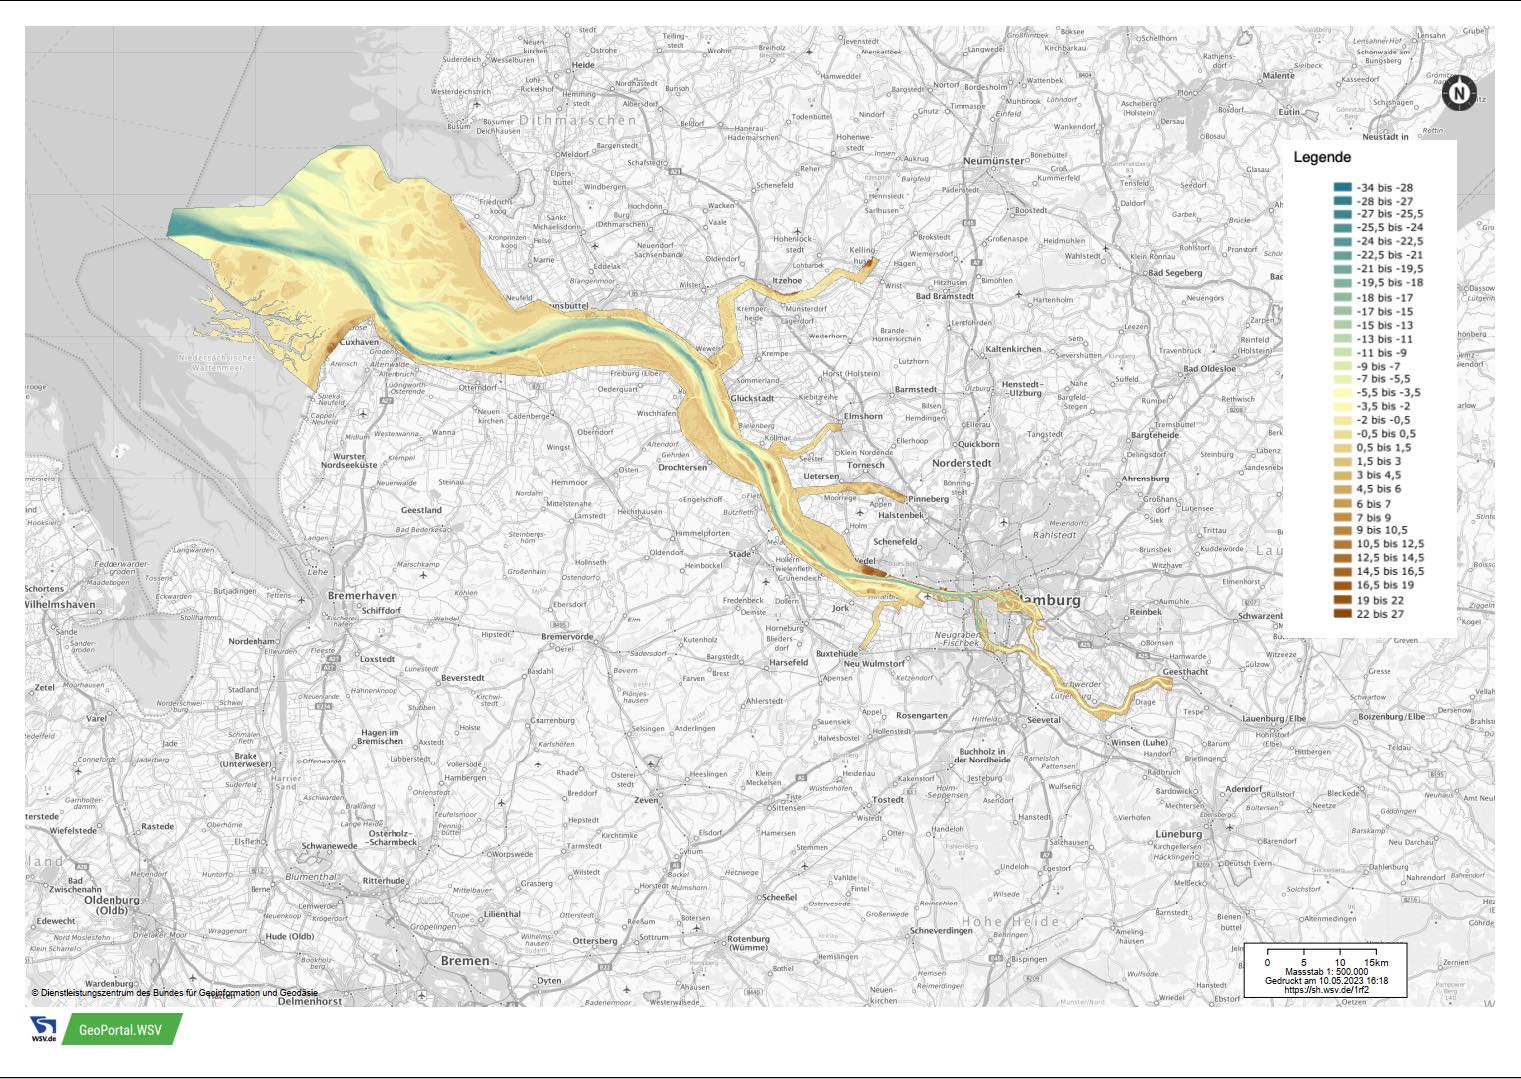
\includegraphics[width=1\textwidth]{figures/Appendix/Map/TopographieElbeGesamt.jpg}
 \caption[Topographic map of Elbe]{Topographic map of the estuary of Elbe. From the Hamburg region to the Waddensea. Scale is in dm, 0 dm is at mean sea level. \cite{ZDMGDWS.2016}}
 \label{TopographyElbeTotal}
\end{figure}
\chapter{Supporting Material for Chapter 3, Results}
\label{cha:app3}
\begin{figure}
\centering
    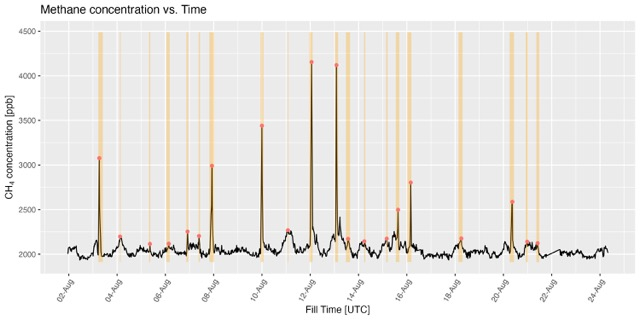
\includegraphics[width=.8\textwidth]{figures/Appendix/CH4_Timelines/MediumPeakTimeline/4_CH4_Timeline0_Medium_Peaks Medium.jpeg}
    \\[\smallskipamount]
    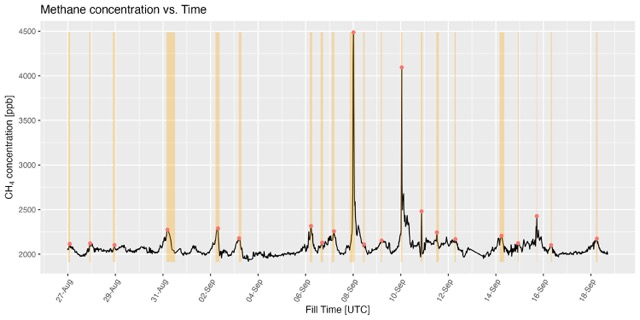
\includegraphics[width=.8\textwidth]{figures/Appendix/CH4_Timelines/MediumPeakTimeline/4_CH4_Timeline1_Medium_Peaks Medium.jpeg}
    \\[\smallskipamount]
    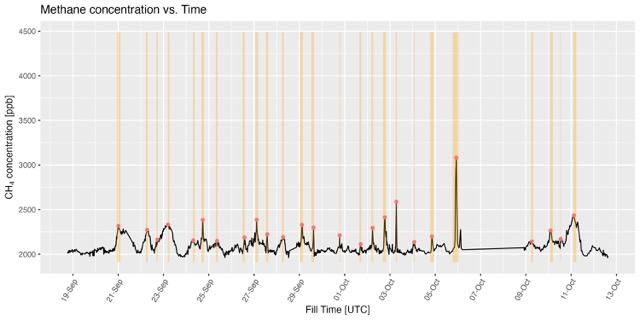
\includegraphics[width=.8\textwidth]{figures/Appendix/CH4_Timelines/MediumPeakTimeline/4_CH4_Timeline2_Medium_Peaks Medium.jpeg}
    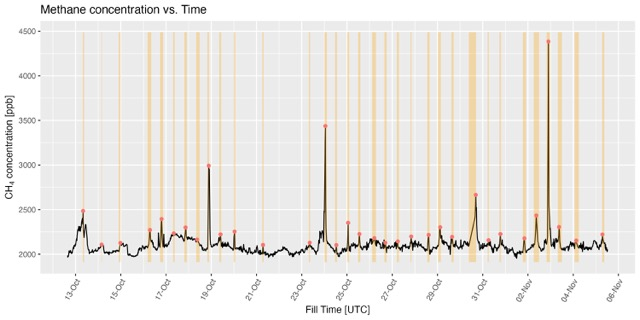
\includegraphics[width=.8\textwidth]{figures/Appendix/CH4_Timelines/MediumPeakTimeline/4_CH4_Timeline3_Medium_Peaks Medium.jpeg}
\end{figure}
\begin{figure} 
\centering
    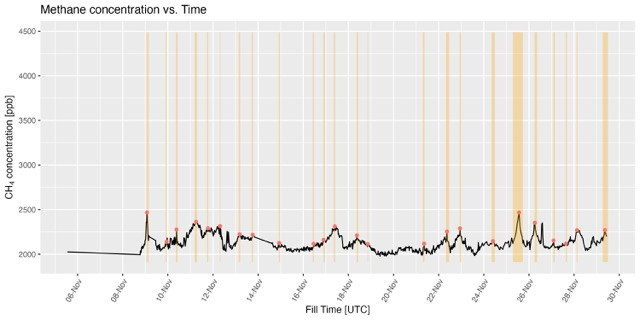
\includegraphics[width=.8\textwidth]{figures/Appendix/CH4_Timelines/MediumPeakTimeline/4_CH4_Timeline4_Medium_Peaks Medium.jpeg}
    \\[\smallskipamount]
    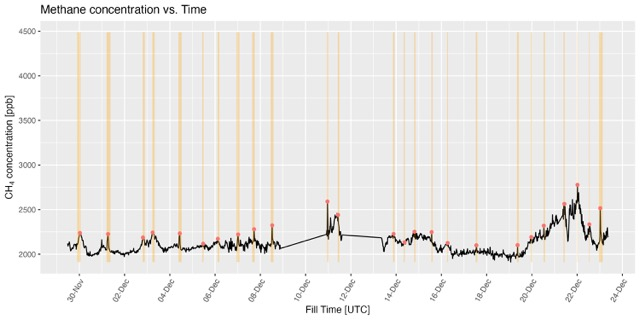
\includegraphics[width=.8\textwidth]{figures/Appendix/CH4_Timelines/MediumPeakTimeline/4_CH4_Timeline5_Medium_Peaks Medium.jpeg}
    \\[\smallskipamount]
    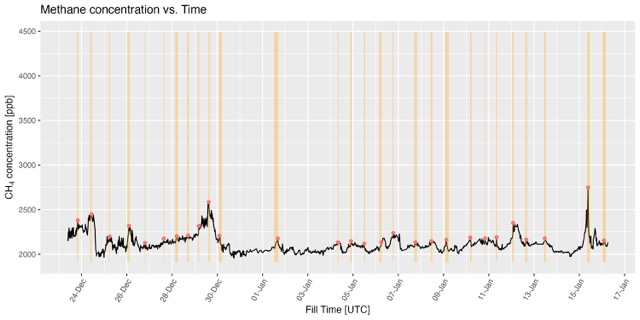
\includegraphics[width=.8\textwidth]{figures/Appendix/CH4_Timelines/MediumPeakTimeline/4_CH4_Timeline6_Medium_Peaks Medium.jpeg}
    \\[\smallskipamount]
    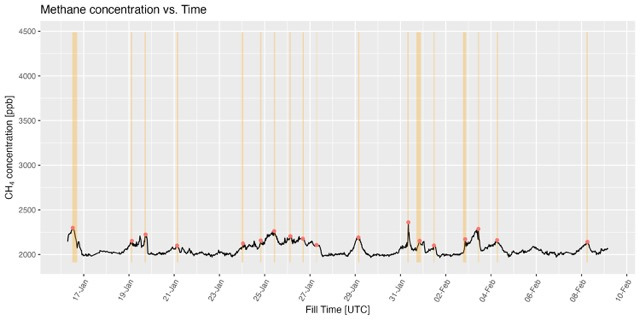
\includegraphics[width=.8\textwidth]{figures/Appendix/CH4_Timelines/MediumPeakTimeline/4_CH4_Timeline7_Medium_Peaks Medium.jpeg}
\end{figure}
\begin{figure}    
\centering
    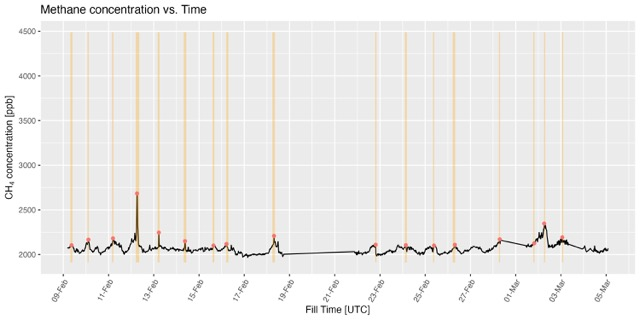
\includegraphics[width=.8\textwidth]{figures/Appendix/CH4_Timelines/MediumPeakTimeline/4_CH4_Timeline8_Medium_Peaks Medium.jpeg}
    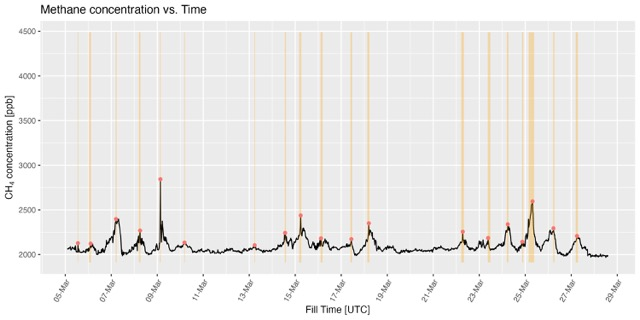
\includegraphics[width=.8\textwidth]{figures/Appendix/CH4_Timelines/MediumPeakTimeline/4_CH4_Timeline9_Medium_Peaks Medium.jpeg}
    \caption[Complete CF-IRMS time-line with prominent peaks highlighted]{Complete CF-IRMS measurement time-line, measured at the Geomatikum at an altitude of 83m above street level. Measurements from  02.08.2021 to 29.03.2021 are shown. Prominent peaks are identified and highlighted. Red dot for peak centre and orange highlight box for peak width.}
    \label{CompleteCF-IRMSTimeinePeaksAppendix}
\end{figure}

\begin{figure}[!htb]
\centering
\begin{subfigure}[b]{0.8\textwidth}
   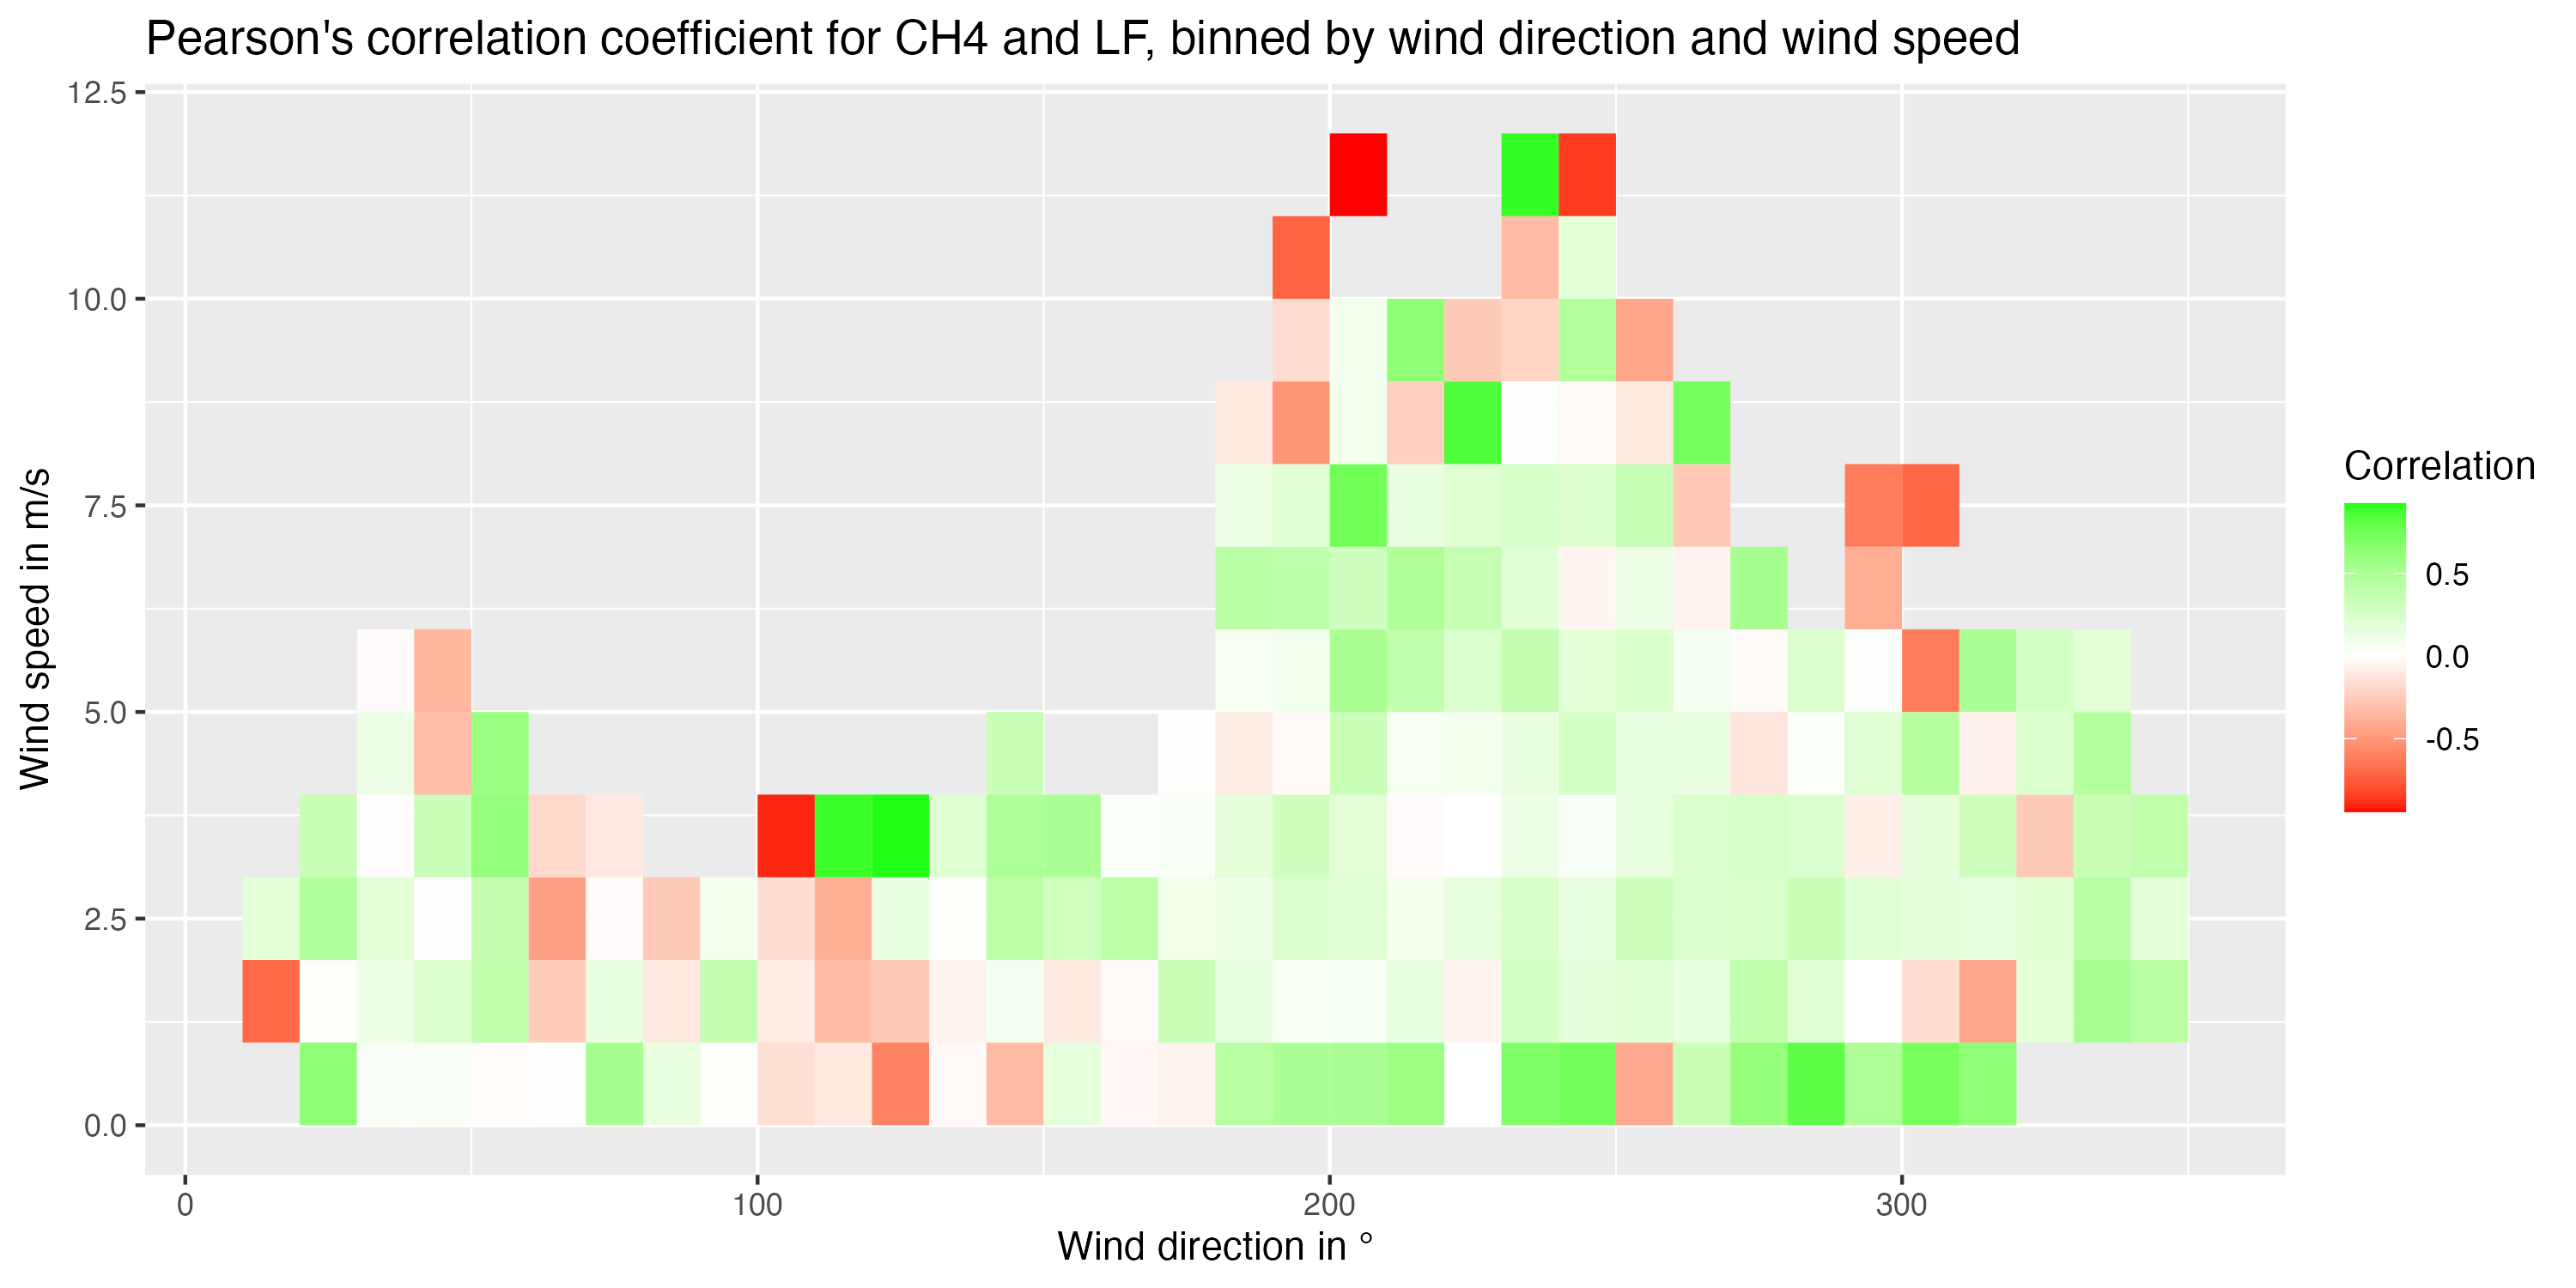
\includegraphics[width=1\linewidth]{figures/Appendix/NoCorrelation/13_CH4_vs_Conductivity_Correlation_Geomatikum.png}
   \caption[NCorrelation plot conductivity in Elbe water]{}
   \label{NoCorrelationConductivity} 
\end{subfigure}
\begin{subfigure}[b]{0.8\textwidth}
   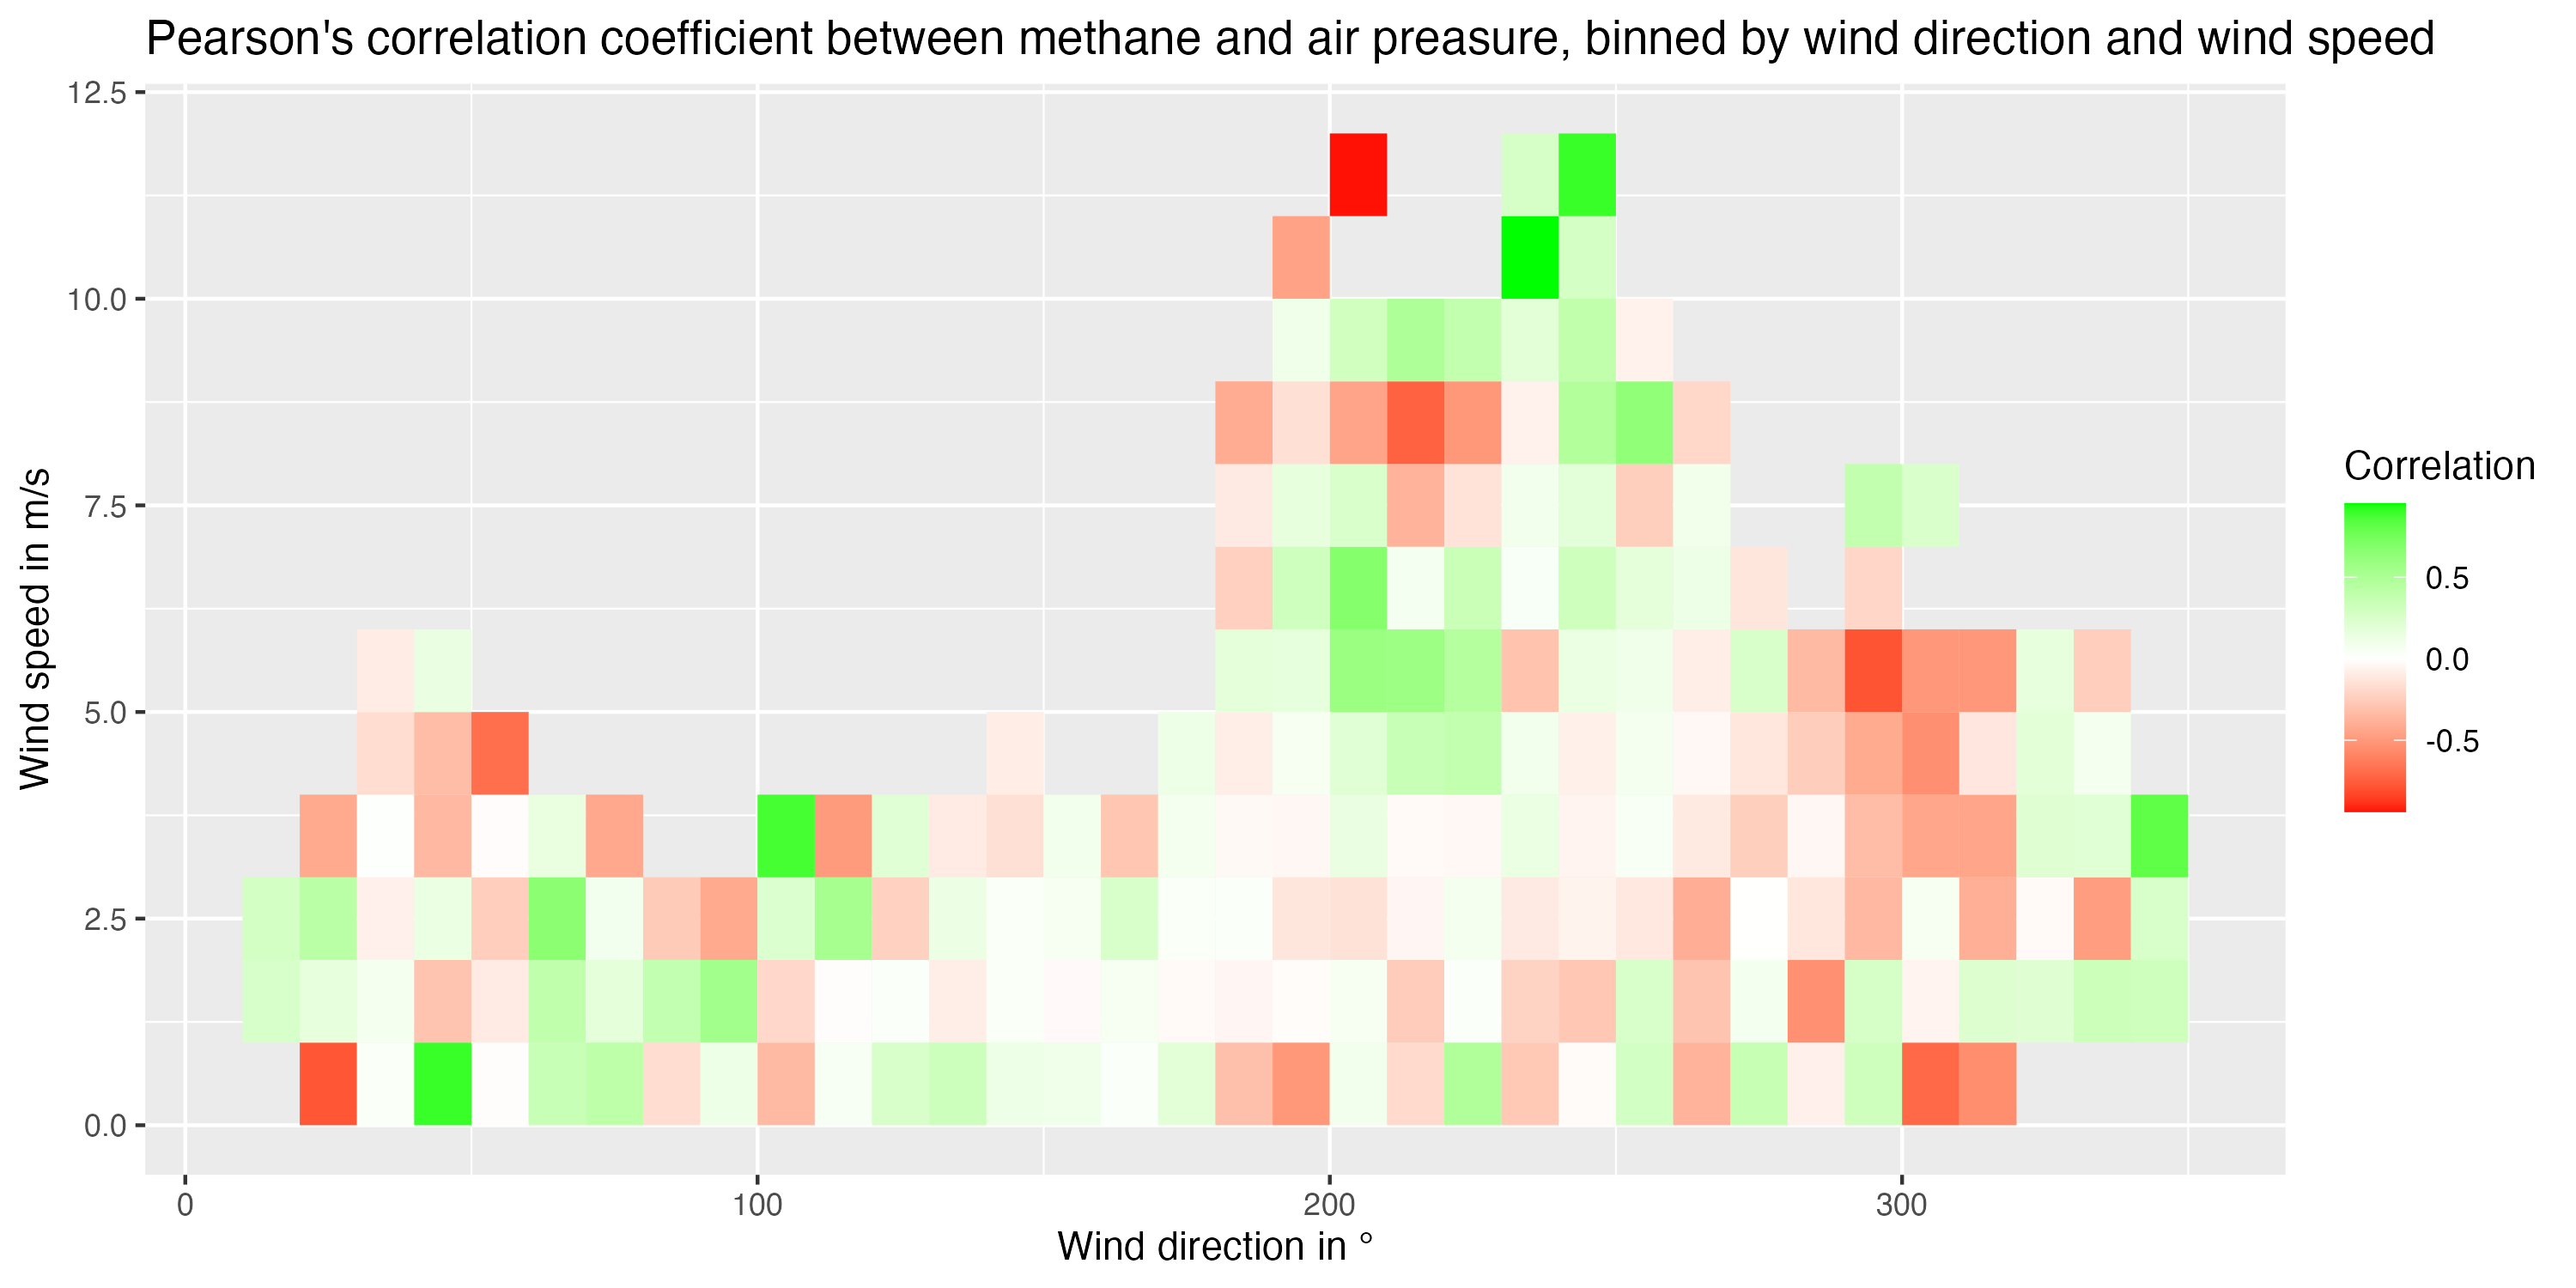
\includegraphics[width=1\linewidth]{figures/Appendix/NoCorrelation/13_CH4_vs_pressure_Correlation_Geomatikum.png}
   \caption[Correlation plot air pressure]{}
   \label{NoCorrelationPressure}
\end{subfigure}
\begin{subfigure}[b]{0.8\textwidth}
   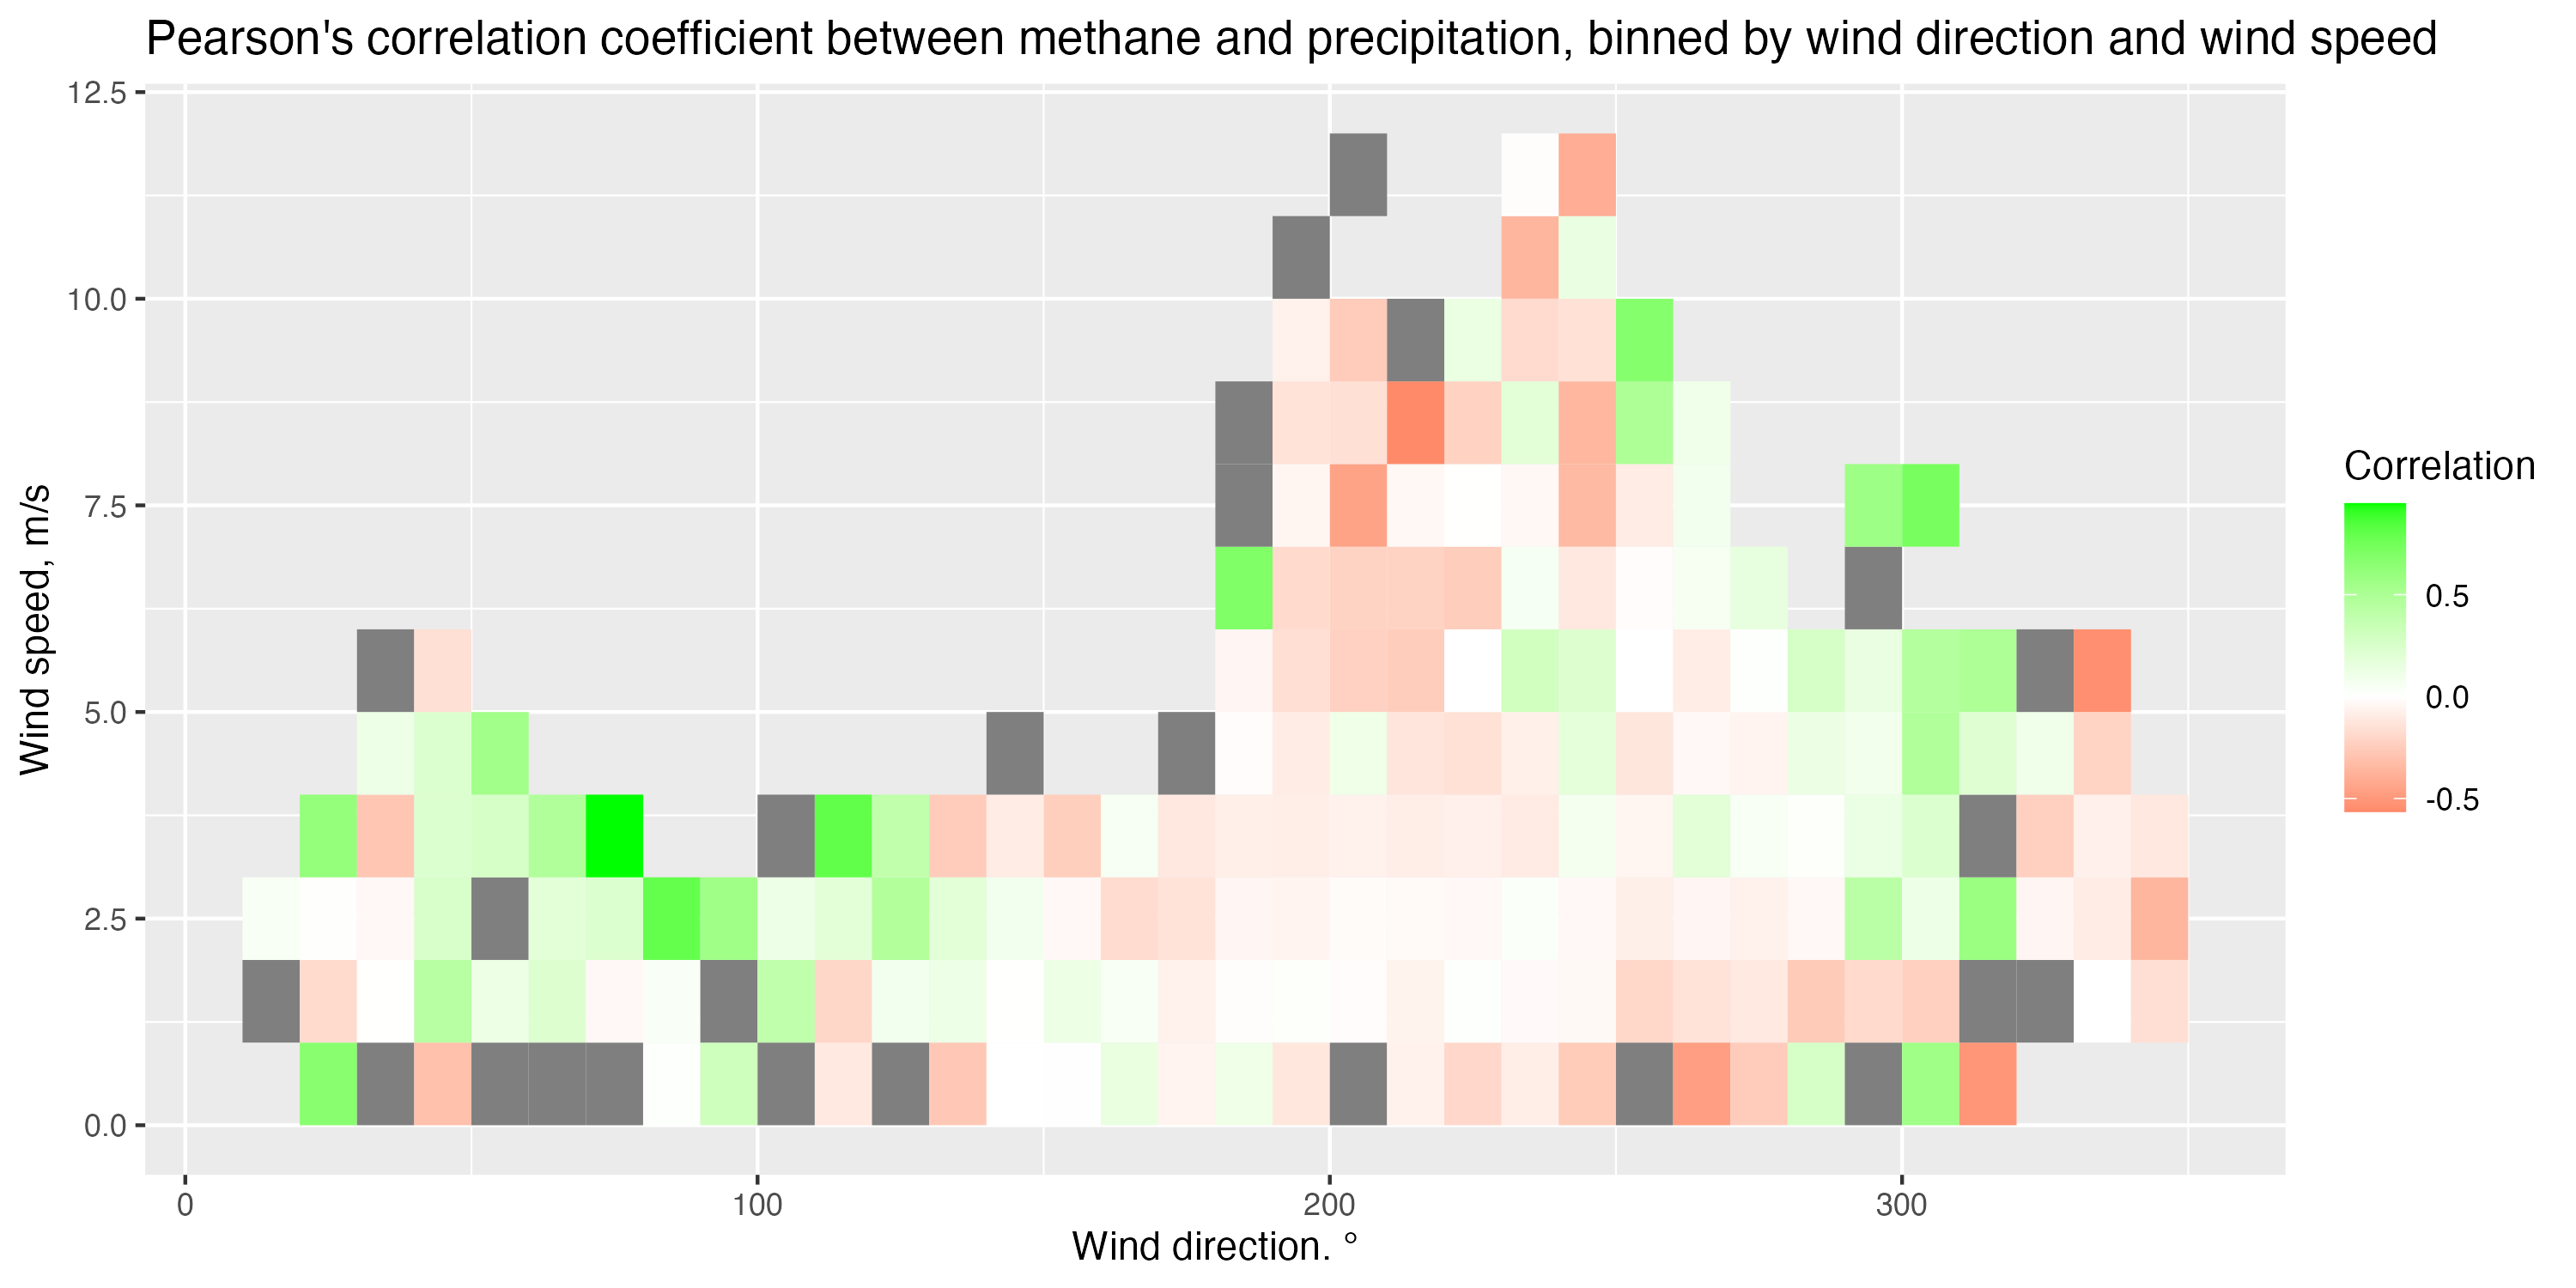
\includegraphics[width=1\linewidth]{figures/Appendix/NoCorrelation/13_CH4_vs_precipitation_height_Correlation_Geomatikum.png}
   \caption[Correlation plot precipitation height]{}
   \label{NoCorrelationPrecipitation}
\end{subfigure}
\caption[Correlation plots showing no correlation with methane concentration in the air]{Pearson's correlation coefficient between methane-air concentration and meteorological/water quality data, binned by wind direction and wind speed. Green shows a positive correlation (enhanced CH$_4$ at high values), and Red shows a negative correlation (enhanced CH$_4$ at low values). (a) Correlation between methane concentration and electrical conductivity in the Elbe water, (b) Correlation betwe(c) Correlation between methane concentration and precipitation height}
\label{NoCorrelationAppendix}
\end{figure}

\begin{figure}[!htb]
\centering
\begin{subfigure}[b]{1\textwidth}
   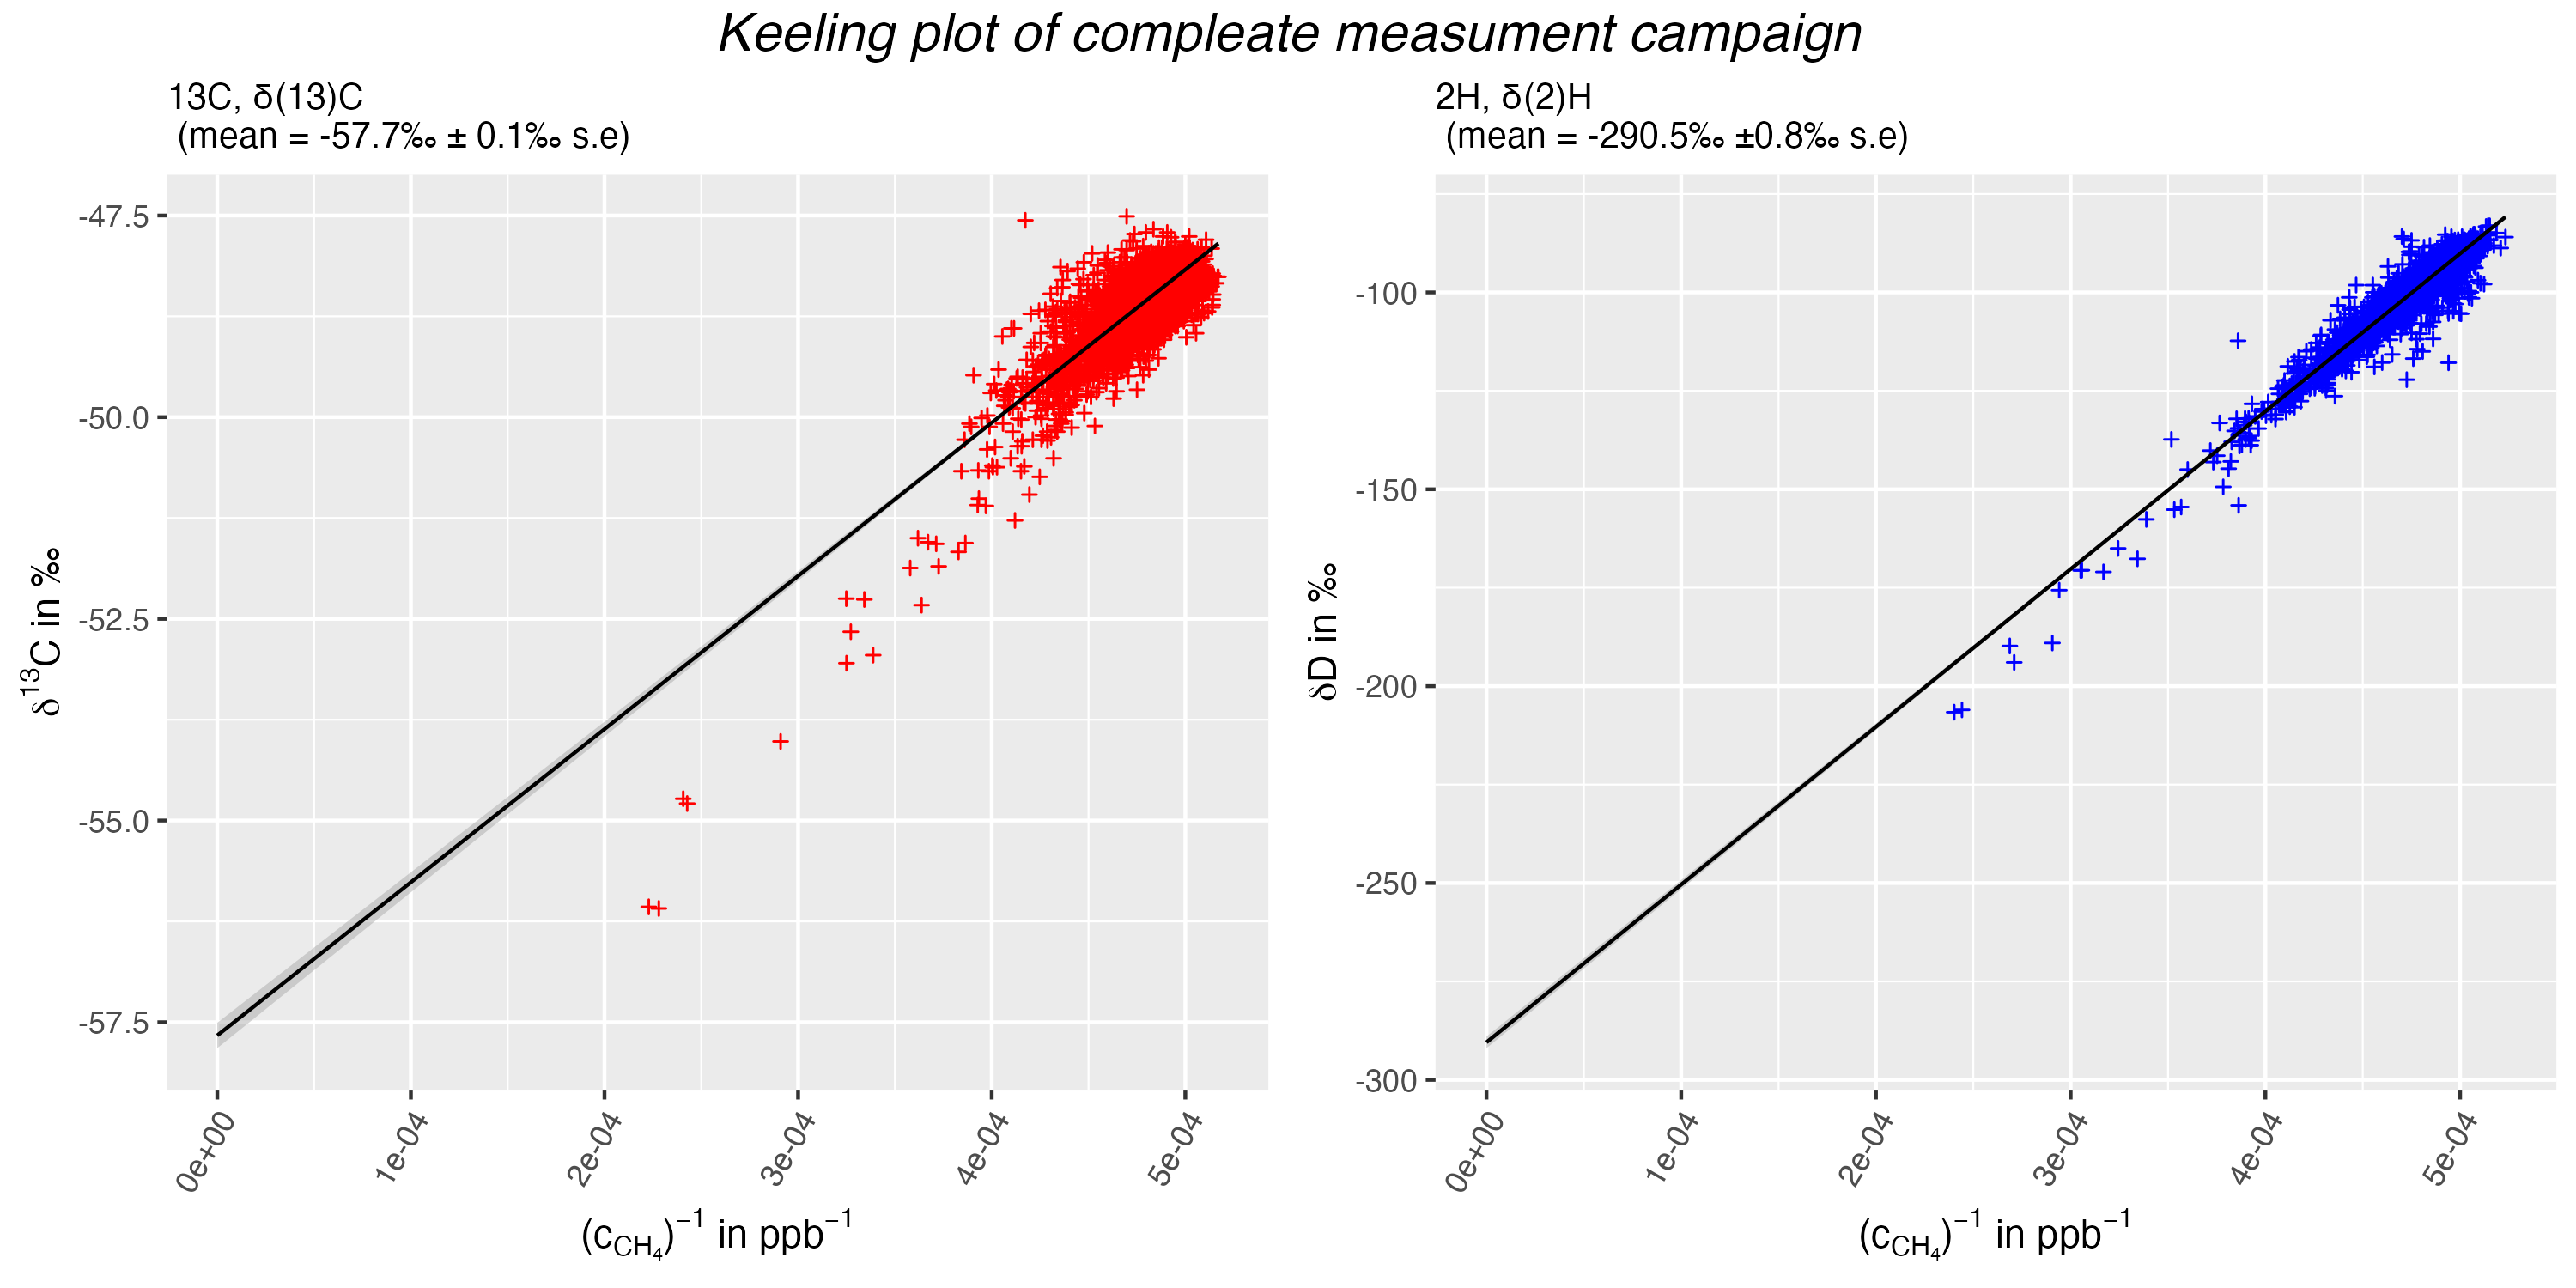
\includegraphics[width=1\linewidth]{figures/Appendix/Keeling/11_Keeling_Plot_Total_paper_peaks.png}
   \caption[Keeling plots total timeline]{}
   \label{KeelingPaperTotal} 
\end{subfigure}

\begin{subfigure}[b]{1\textwidth}
   \includegraphics[width=1\linewidth]{figures/Appendix/Keeling/11_Keeling_Plot_Peaks_paper_peaks.png}
   \caption[Keeling plots literature peak identification criteria]{}
   \label{KeelingPaperPeaks}
\end{subfigure}

\caption[Keeling Plot for CH$_4$ peaks in CR-IRMS measurement with peak identification criteria from literature]{Keeling Plots of Carbon-13 and Deuterium in methane peaks measured at the Geomatikum from 1.08.2021 to 1.04.2022. (a) total timeseries with resulting isotopic signatures $\delta$13C = -57.7$\permil$ and $\delta$D = -200.5$\permil$. (b) peak identification criteria by \cite{Menoud.2021}. The resulting isotopic signatures $\delta$13C = -58.1$\permil$ and $\delta$D = -291.2$\permil$}
\label{KeelingPaper}
\end{figure}

\begin{figure}[htbp]
\centering
\begin{subfigure}[b]{1\textwidth}
   \includegraphics[width=1\linewidth]{figures/Appendix/Keeling/12_Keeling_Total_Wind_paper_peaks.png}
   \caption{}
   \label{DualIsotiotopePaperTotal} 
\end{subfigure}
\begin{subfigure}[b]{1\textwidth}
   \includegraphics[width=1\linewidth]{figures/Appendix/Keeling/12_Keeling_Peaks_Wind_paper_peaks.png}
   \caption{}
   \label{DualIsotiotopePaperPeaks}
\end{subfigure}
\caption[Dual isotope plot with Literature peak identification criteria]{Dual isotope plot for CF-IRMS measurement for 10° wind direction represented as point colour(blue towards North, red toward South) with highlighted production mechanism (coloured highlight) and source type (coloured boxes). Error bars show one SD. (a) shows total time series, (b) shows only peaks selected with identification criteria by \cite{Menoud.2021}}
\label{DualIsotiotopePlotsAppendix}
\end{figure}

\begin{table}[htbp]
\centering
\begin{tabular}{@{}lllll@{}}
\toprule
W. Direction & $\delta$13C & SE $\delta$13C & $\delta$D & SE $\delta$D \\ \midrule
10        & -49.       & 8.0      & -191      & 2.5     \\
20        & -50.       & 1.9      & -257      & 13.     \\
30        & -52.       & 0.6      & -265      & 6.9     \\
40        & -51.       & 1.0      & -266      & 5.7     \\
50        & -52.       & 0.85     & -261      & 10.     \\
60        & -50.       & 1.1      & -267      & 15.     \\
70        & -49.       & 1.2      & -248      & 13.     \\
80        & -52.       & 0.99     & -279      & 10.     \\
90        & -53.       & 1.3      & -2        & 15.     \\
100       & -53.       & 1.5      & -253      & 30.     \\
110       & -51.       & 1.6      & -255      & 14.     \\
120       & -53.       & 1.2      & -268      & 10.     \\
130       & -52.       & 1.1      & -262      & 9       \\
140       & -51.       & 0.90     & -262      & 8.5     \\
150       & -51.       & 0.9      & -239      & 9.0     \\
160       & -55.       & 0.91     & -255      & 12.     \\
170       & -54        & 0.       & -283      & 6.      \\
180       & -59        & 0.27     & -290      & 3.7     \\
190       & -58.       & 0.23     & -298      & 2.3     \\
200       & -57.       & 0.2      & -290      & 1.9     \\
210       & -59.       & 0.22     & -285      & 2.4     \\
220       & -5         & 0.26     & -294      & 2.0     \\
230       & -57.       & 0.3      & -289      & 3.1     \\
240       & -57.       & 0.32     & -299      & 2.7     \\
250       & -57.       & 0.32     & -299      & 2.8     \\
260       & -57.       & 0.28     & -291      & 2.7     \\
270       & -58        & 0.33     & -289      & 2.8     \\
280       & -56.       & 0.51     & -30       & 4.3     \\
290       & -58.       & 0.43     & -29       & 5.2     \\
300       & -56.       & 0.68     & -283      & 7.5     \\
310       & -55.       & 0.96     & -273      & 7.2     \\
320       & -54.       & 0.75     & -283      & 9.4     \\
330       & -56.       & 0.74     & -281      & 6.6     \\
340       & -54.       & 1.0      & -28       & 7.6     \\
350       & -55.       & 3.2      & -273      & 22.     \\ \bottomrule
\end{tabular}
\label{WindKeelingTableTotalAppendix}
\caption[Windrose by DWD and Universität Hamburg]{Table of isotopc signature of $\delta$13C and $\delta$D by Keeling analyse for the total CF-IRMS measurement at the Geomatikum, 01.08.2022 to 01.03.2022, separated in wind directions during the measurement.}
\end{table}


\begin{figure}\centering
\subfloat[]{\label{WindRoseDWD}\includegraphics[width=.45\linewidth]{figures/Appendix/Windrose/WindRose_Total_DWD.png}}\hfill
\subfloat[]{\label{WindRose50m}\includegraphics[width=.45\linewidth]{figures/Appendix/Windrose/WindRose_Total_50m.png}}\par 
\subfloat[]{\label{WindRose110m}\includegraphics[width=.45\linewidth]{figures/Appendix/Windrose/WindRose_Total_110m.png}}
\caption[Windrose by DWD and Universität Hamburg]{Windrose plots with data from (a) Deutscher Wetterdienst (DWD) (\cite{DeutschenWetterdienst.20230501}) at Fuhlsbüttel, Hamburg and Universität Hamburg \cite{Lange.20220501} with wind measurements at (b) 50 m and (c) 110m}
\label{WindRoseAppendix}
\end{figure}




\begin{figure}[htbp]
 \centering
 \includegraphics[width=1\textwidth]{figures/Appendix/Transportmodel/14_Low_WL_to_Peak_distance_paper_peaks.png}
 \caption[Distance between estimated emitter and measurement location]{Scatter plot of modelled Distance between the estimated emission location and the measurement location at the Geomatikum, against the methane concentration observed at the Geomatikum measured by the CF-IRMS. A local regression line is fitted to the plot (Blue). The standard error of the line is shown in dark grey. The peaks were identified using the identification criteria by \cite{Menoud.2021}}
 \label{DistancePlotPaperAppendix}
\end{figure}

\begin{figure}[htbp]
\centering
\begin{subfigure}[b]{1\textwidth}
   \includegraphics[width=1\linewidth]{figures/Appendix/FTIR/15_Basic_Plot_CH4_Wl_FTIR202108031mc.png}
   \caption{}
   \label{FTIRWLJork} 
\end{subfigure}
\begin{subfigure}[b]{1\textwidth}
   \includegraphics[width=1\linewidth]{figures/Appendix/FTIR/15_Basic_Plot_CH4_Wl_FTIR202108031md.png}
   \caption{}
   \label{FTIRWLRosengarten}
\end{subfigure}
\caption[FTIR with water level overlay timeline]{Plot of the total column methane concentration measured (Red line) overlayed with the Elbe water level measured at St.
Pauli (Black line). The measurements were performed on 31.08.2021. (a) measured at Jork, (b) measured at Rosengarten. A low water methane peak can be seen at 16:00 UTC.}
\label{FTIRWLAppendix}
\end{figure}


\addcontentsline{toc}{chapter}{\protect Bibliography}
\bibliography{MasterArbeit_File}

\addcontentsline{toc}{chapter}{\protect List of Figures}
\listoffigures

\addcontentsline{toc}{chapter}{\protect List of Tables}
\listoftables







\end{document}